\documentclass[12pt,letterpaper]{article}
%\usepackage{preamble}

%\ProvidesPackage{preamble}

\usepackage{fullpage}
\usepackage[top=2cm, bottom=4.5cm, left=2.5cm, right=2.5cm]{geometry}
\usepackage{amsmath,amsthm,amsfonts,amssymb,amscd}
\usepackage{lastpage}
\usepackage{enumerate}
\usepackage{fancyhdr}
\usepackage{mathrsfs}
\usepackage{xcolor}
\usepackage{graphicx}
\usepackage{listings}
\usepackage{hyperref}
\usepackage{enumitem}
\usepackage{float}
\usepackage{fancyvrb}
\usepackage{color,soul}
\sethlcolor{lightgray}
 \usepackage{subfigure}
 \usepackage{textcomp}
\usepackage{siunitx}

\usepackage{graphicx}
\usepackage{array}

\usepackage[T1]{fontenc}
\usepackage[numbered,framed]{matlab-prettifier}
\hypersetup{%
  colorlinks=true,
  linkcolor=blue,
  linkbordercolor={0 0 1}
}

\let\ph\mlplaceholder % shorter macro
\lstMakeShortInline"

\lstset{
  style              = Matlab-editor,
  basicstyle         = \mlttfamily \small,
  escapechar         = ",
  mlshowsectionrules = true,
  xleftmargin=.01\textwidth, xrightmargin=.01\textwidth
}

\graphicspath{{./problem1_images}}

\pagestyle{fancyplain}
\headheight 35pt
\lhead{\userID}
\chead{\textbf{\Large Project \hwnumber}}
\rhead{\course \\ \today}
\lfoot{}
\cfoot{}
\rfoot{\small\thepage}
\headsep 1.5em




%%%%%%%%%%%%%%%%%%%%%%%%%%%%%%%%%%%%%%%%%%
%%%% Edit These for yourself
%%%%%%%%%%%%%%%%%%%%%%%%%%%%%%%%%%%%%%%%%%
\newcommand\course{Econ 672}
\newcommand\hwnumber{3}
\newcommand\userID{Ziming Huang}
\newenvironment{alphaparts}[0]{%
  \begin{enumerate}[label=\textbf{\Alph*}]
}{\end{enumerate}}


\begin{document}

\section*{Exercise 1}
  \begin{enumerate}[label=\textbf{(\Alph*)}]
%----A-----
  \item To compute the time-of-day-factor, we need to do the following steps:
 	 \begin{enumerate}[label=(\roman*)]
  	    \item Use log-price $X_{t,i}$ to calculate log-return $r_{t,i}$;
  	    \item Use this formula to calculate variable $b_i$: $b_i=\frac{1}{T}\sum_{t=1}^{T}|r_{t,i}|\times |r_{t,i-1}|$, for ${i=2,3,\dots,n}$;
  	    \item Set $b_1=b_2$ and use $b_i$ to calculate time-of-day-factor $\tau_i$: $\tau_i=\frac{b_i}{\frac{1}{n}\sum_{j=1}^{n}b_j}$, for ${i=1,2,3,\dots,n}$.
  	\end{enumerate}
  Here is the plot of time-of-day-factor:
  \begin{figure}[H]
           \subfigure{
           \begin{minipage}[l]{1\linewidth}
           \centering
            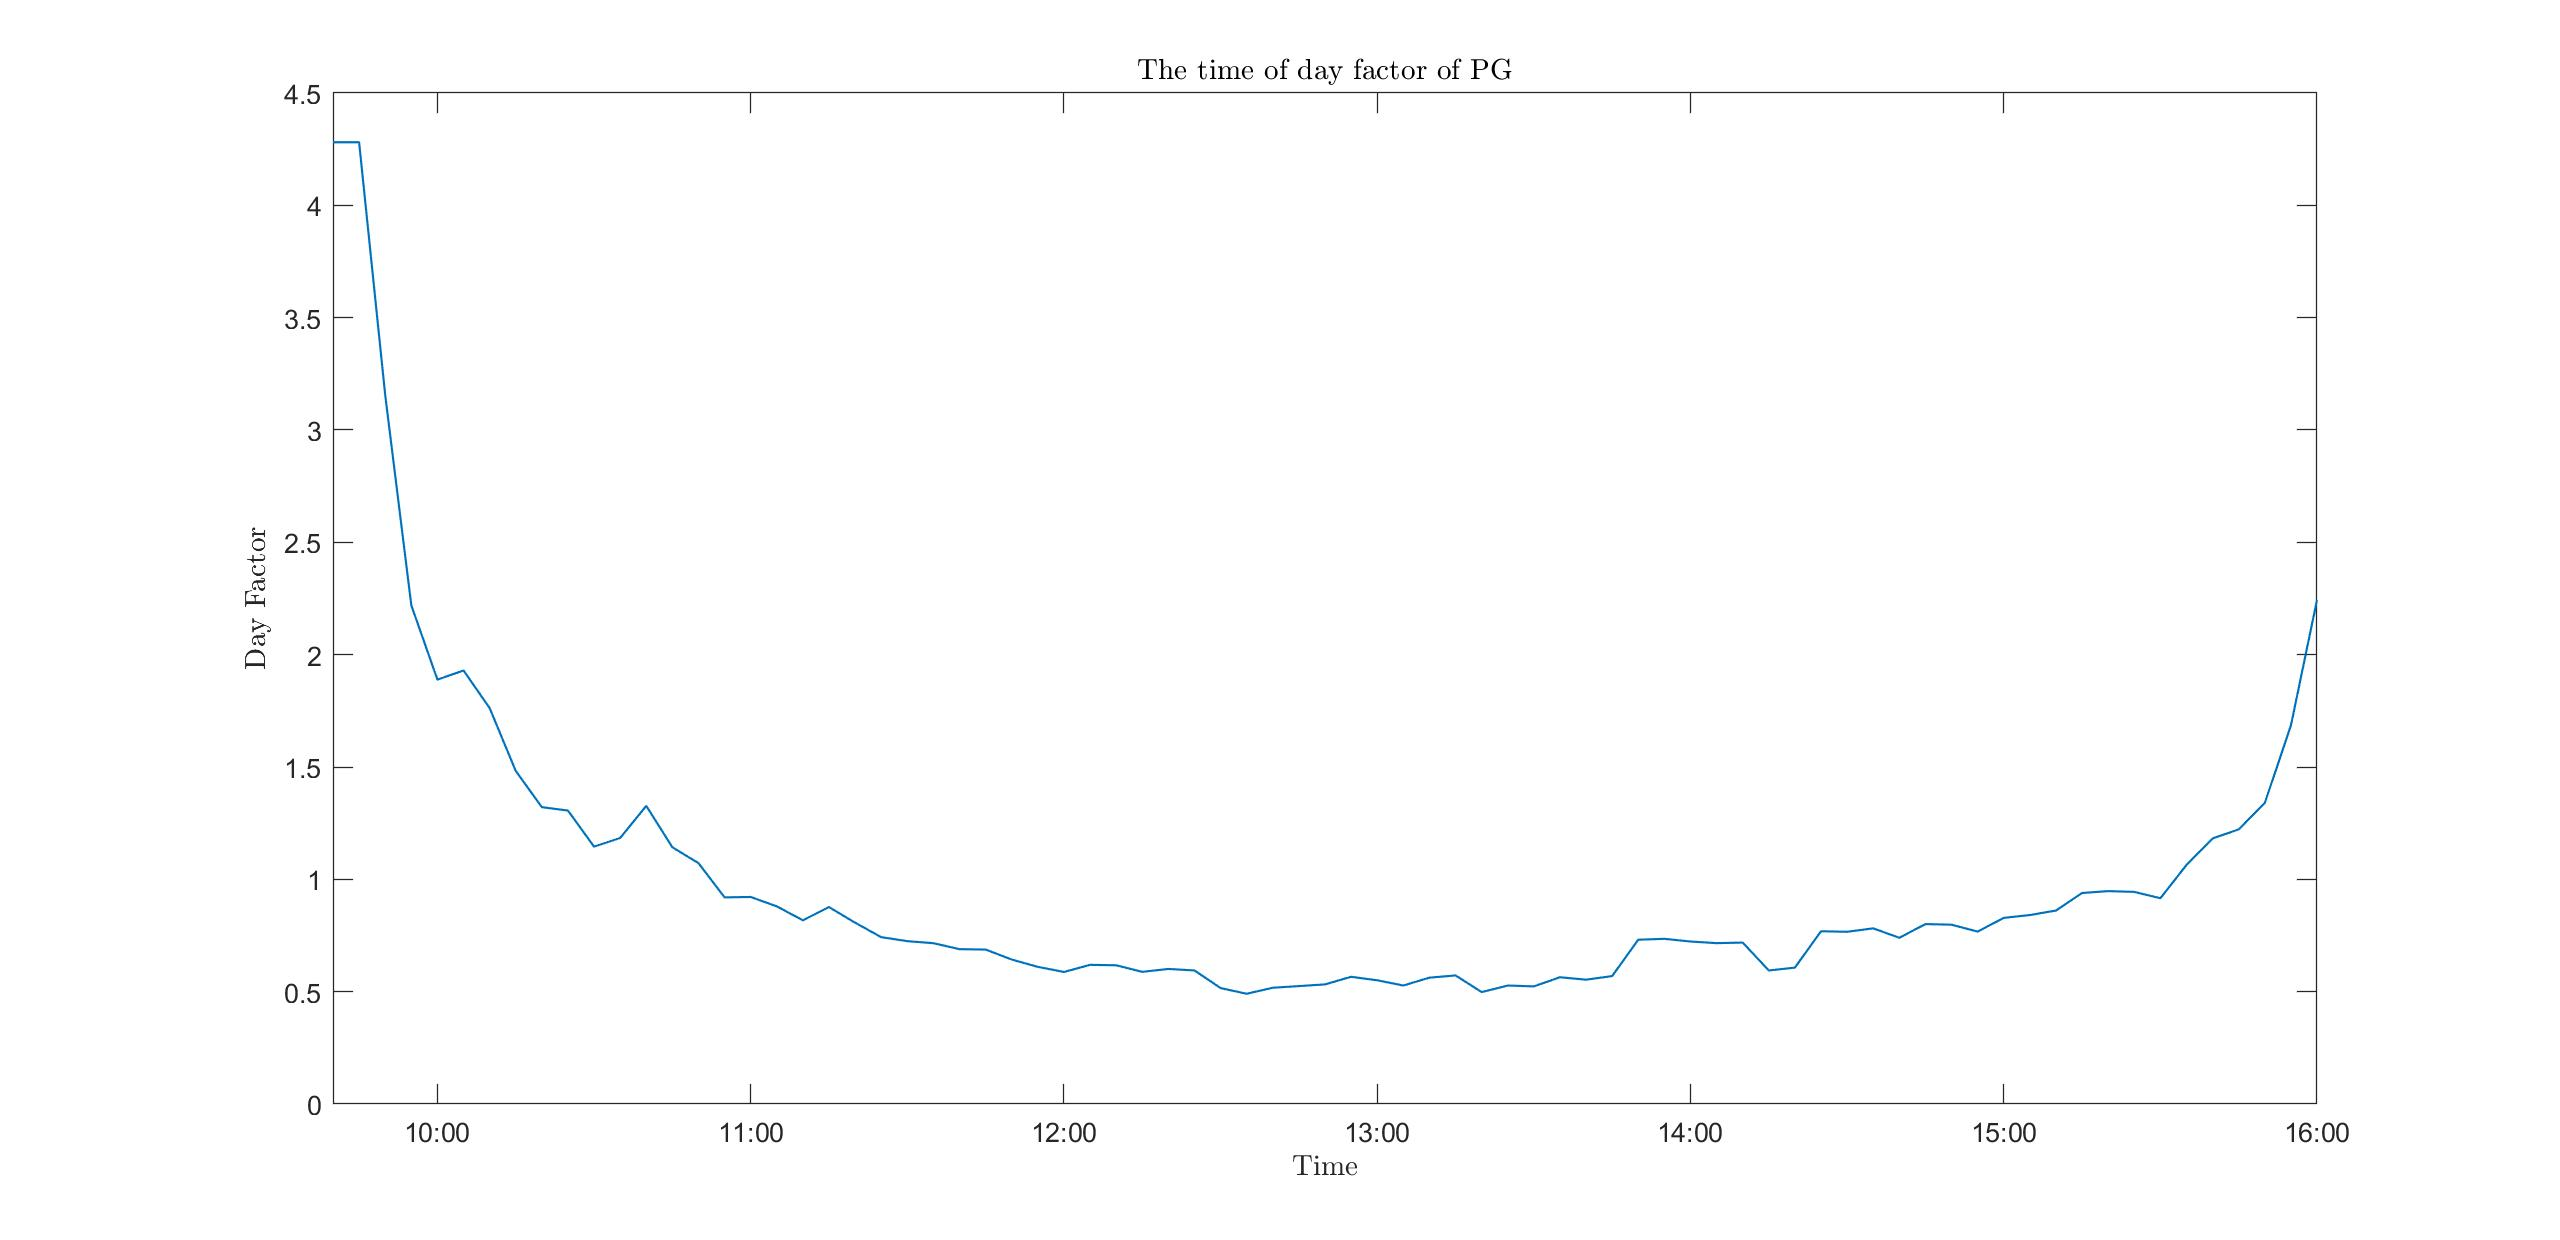
\includegraphics[width=3in]{figures/p3_ex1_a.jpg}
            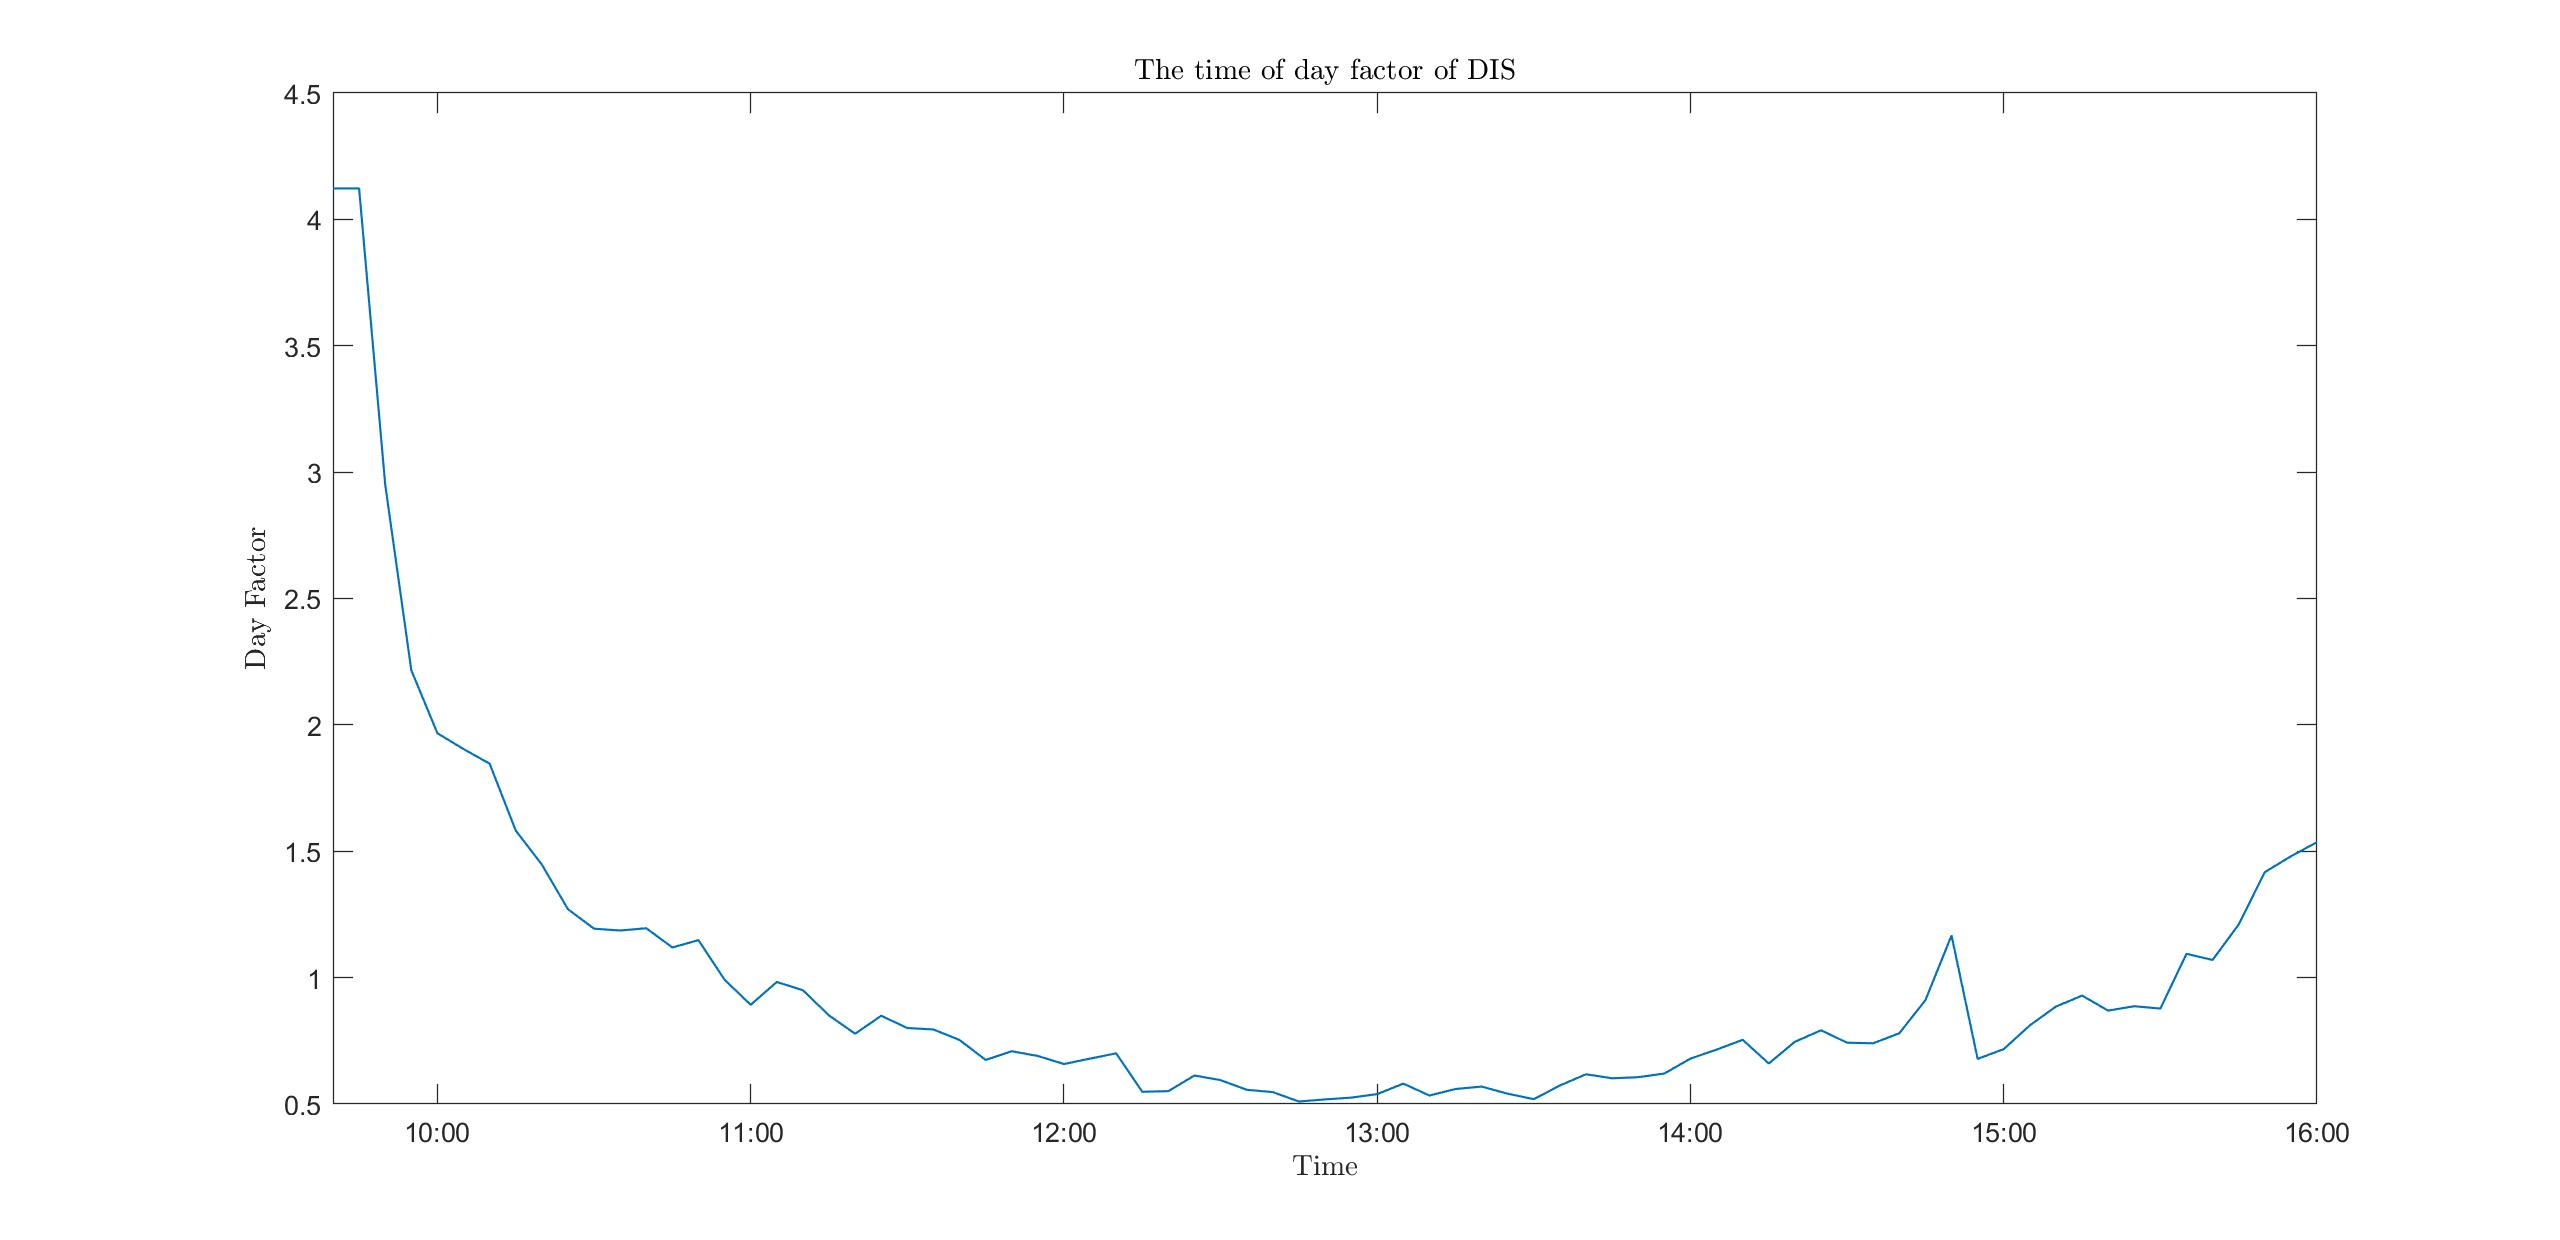
\includegraphics[width=3in]{figures/p3_ex1_a_DIS.jpg}
            \end{minipage}
            }
            \centering
            \caption{Time-of-day-factor for PG and DIS}
\end{figure}
From these figures, we can see that the range of time-of-day-factor of PG and DIS are (0.5, 4.3) and (0.5, 4.1) respectively. The curve of PG's time-of-day-factor is smoother than the curve of DIS'. We can also find at DIS' figure, the time-of-day-factor has a small peak at around 15:00, which does not show in PG' figure.\\

Both PG and DIS have a U-shape time-of-day-factor: at the early time of trade hours, the time-of-day-factor is very large and then shows a trend of decreasing; at the middle of trading hours, the time-of-day-factor reaches its lowest value; then the time-of-day-factor begins to increase till the end of the trading hours. Even though the time-of-day-factor shows a upside trend after middle trading hours, the highest value it can reach is still smaller than the time-of-day-factor at the very beginning of the trading day.  \\

   The \textbf{MATLAB} code:
   \lstinputlisting{functions/time_of_day_factor.m}
   ~~\\

%-----B-----
\item Lee and Mykland (2006)\footnote{Lee, S. S., and P. Mykland (2006). Jumps in Financial Markets: A New Nonparametric Test and Jump Dynamics. Working Paper. Georgia Institute of Technology and University of Chicago.} have found that the jumps are more frequency happens within the 9:30 to 10:30. Tassel(2007)\footnote{P. Van Tassel. Patterns Within the Trading Day: Volatility and Jump Discontinuities
in High-Frequency Equity Price Series. Duke University Senior Honors Thesis, 2009.} shows that: ``The number of flagged jumps also begins to increase later in the trading day, a potential response to the Federal Open Market Committee statements that are released at approximately 2:15pm''. 

The frequency jumps may be the reason to cause the volatility much higher at the begin of trading hours. McInish and Ord in their paper(1985)\footnote{Wood, R. A., T. H. McInish, and J. K. Ord (1985). An investigation of transaction data for NYSE stocks. \emph{Journal of Finance}, 25, 723-739.}have discovered that the price of individual stock price volatility intraday shows U-shape pattern. The U-shape pattern of price volatility means that the volatility of stock price will follow the distribution with different variance. 

Since we want to use the bi-power variance as a estimator of price's really volatility, in order to make this estimator more efficient, we need to multiple a parameter to adjust the value of bi-power variance and to let it match the small intervals' variance. The parameter we use is the time-of-day-factor. Since the function of the time-of-day-factor is to help us to estimate the variance with day, the shape of time-of-day-factor with share the same pattern of the volatility of price intraday. If the volatility of intraday price does not have the pattern of U-shape of it is just show a reasonable flat pattern, then our day-of-time-factor will have a constant pattern or similar. \\

%----C----
\item To separate the diffusive returns from jump returns, we have the following steps;
   \begin{enumerate}[label=(\roman*)]
  	    \item Calculate $BV_t$ to estimate the returns volatulity;
  	    \item Choose the number of $\sigma$ that we want to bound our diffusive returns(i.e. $\alpha$);
  	    \item Use this formula to calculate our cut\_off matrix: $\alpha\Delta_n^0.49\sqrt{\tau_iBV_t}$;
  	    \item Use cut\_off matrix as indicator to separate diffusive returns and jump returns:
 	\end{enumerate} 
 	
We can verify that $r_{t,i}=r_{t,i}^c+r_{t,i}^d$ by using the code: \hl{k=sum((diffusive return(:)+jump return(:)==regular(:)))}. We have k=0, which means for every element in regular log returns, it will equal to diffusive return plus jump return.
 	
 Here are the plots of diffusive returns and jump returns for PG and DIS:
   \begin{figure}[H]
           \subfigure{
           \begin{minipage}[l]{1\linewidth}
           \centering
            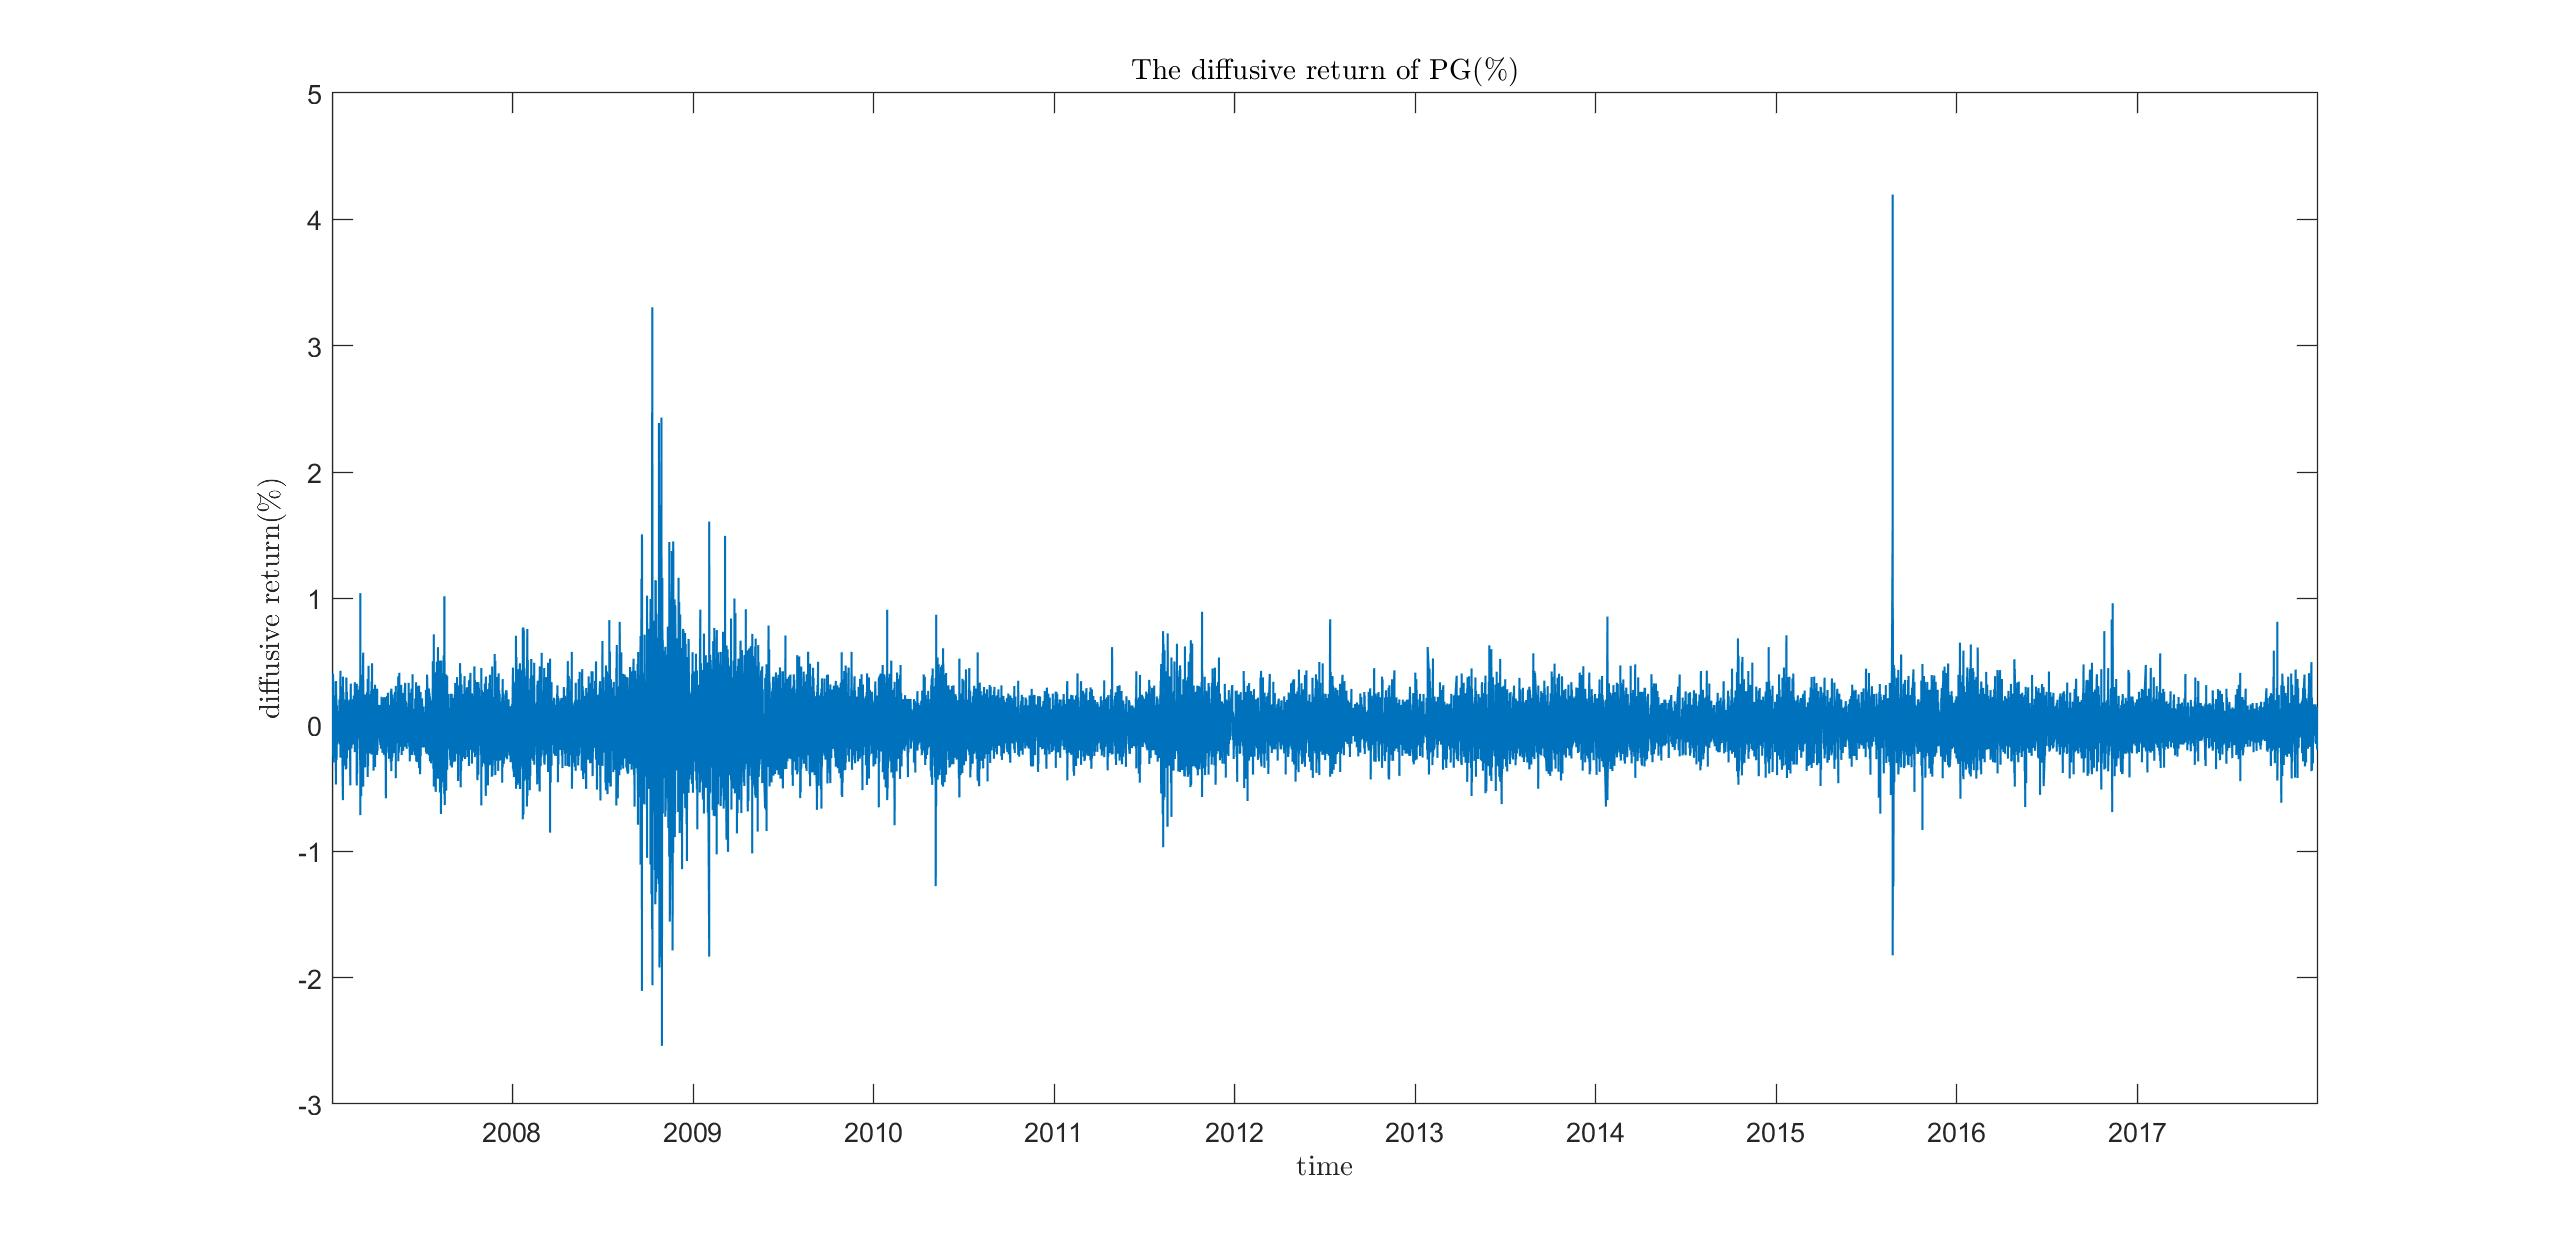
\includegraphics[width=3in]{figures/p3_ex1_c_c.jpg}
            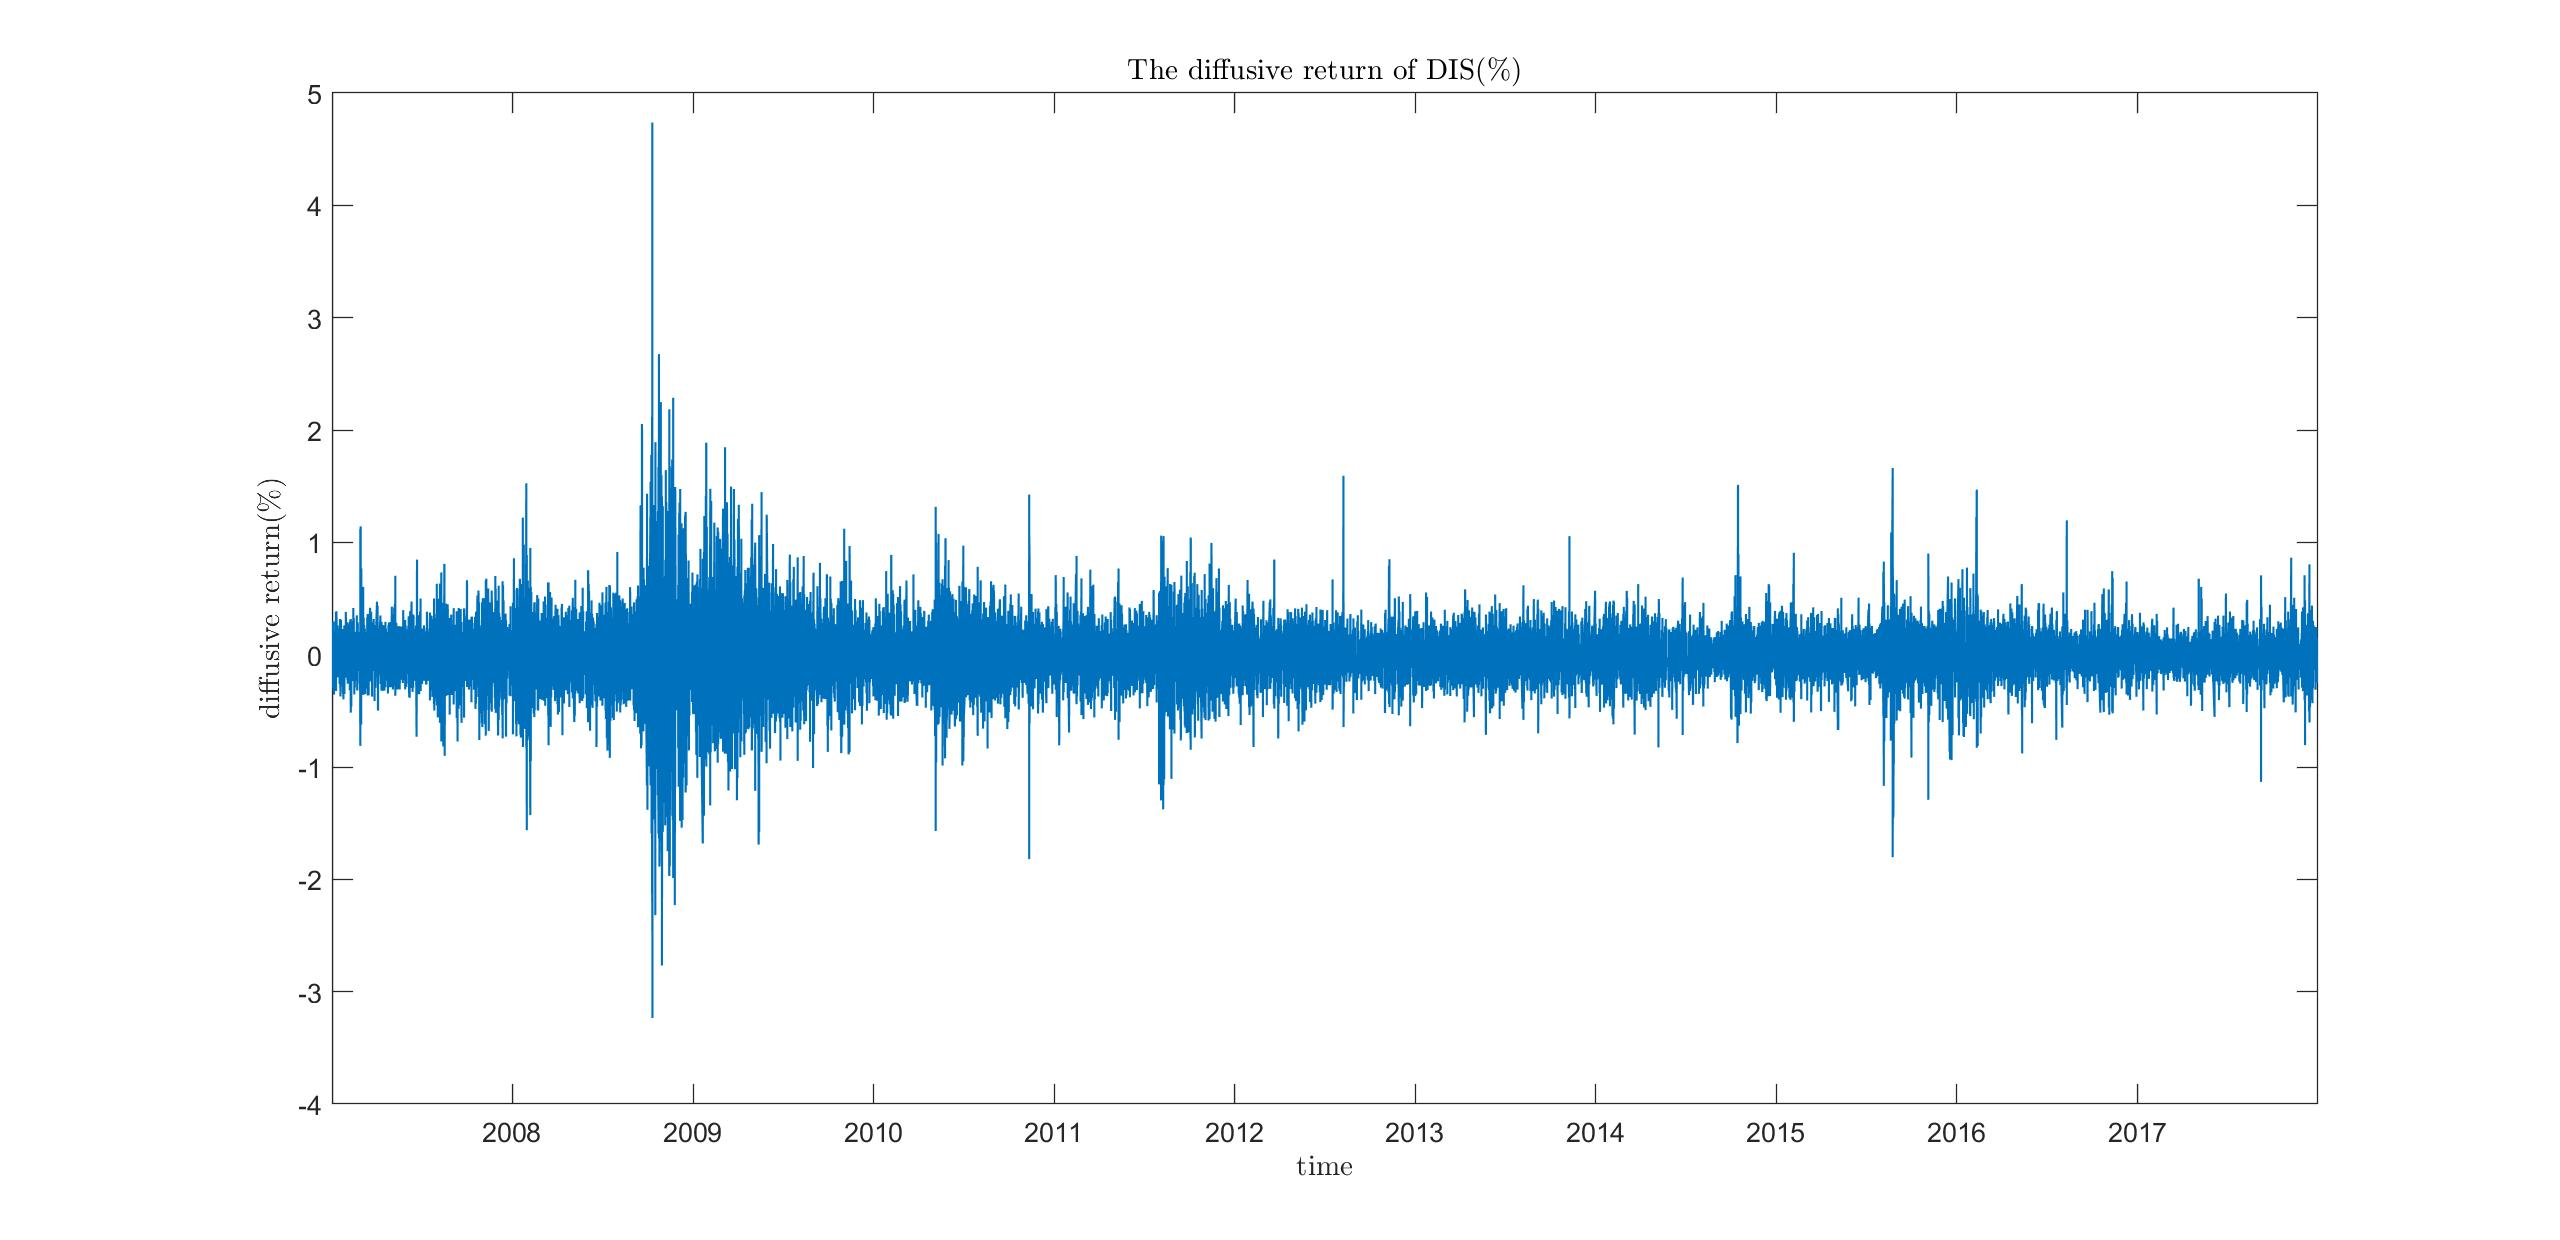
\includegraphics[width=3in]{figures/p3_ex1_c_c_DIS.jpg}
            \end{minipage}
            }
             \subfigure{
           \begin{minipage}[l]{1\linewidth}
           \centering
            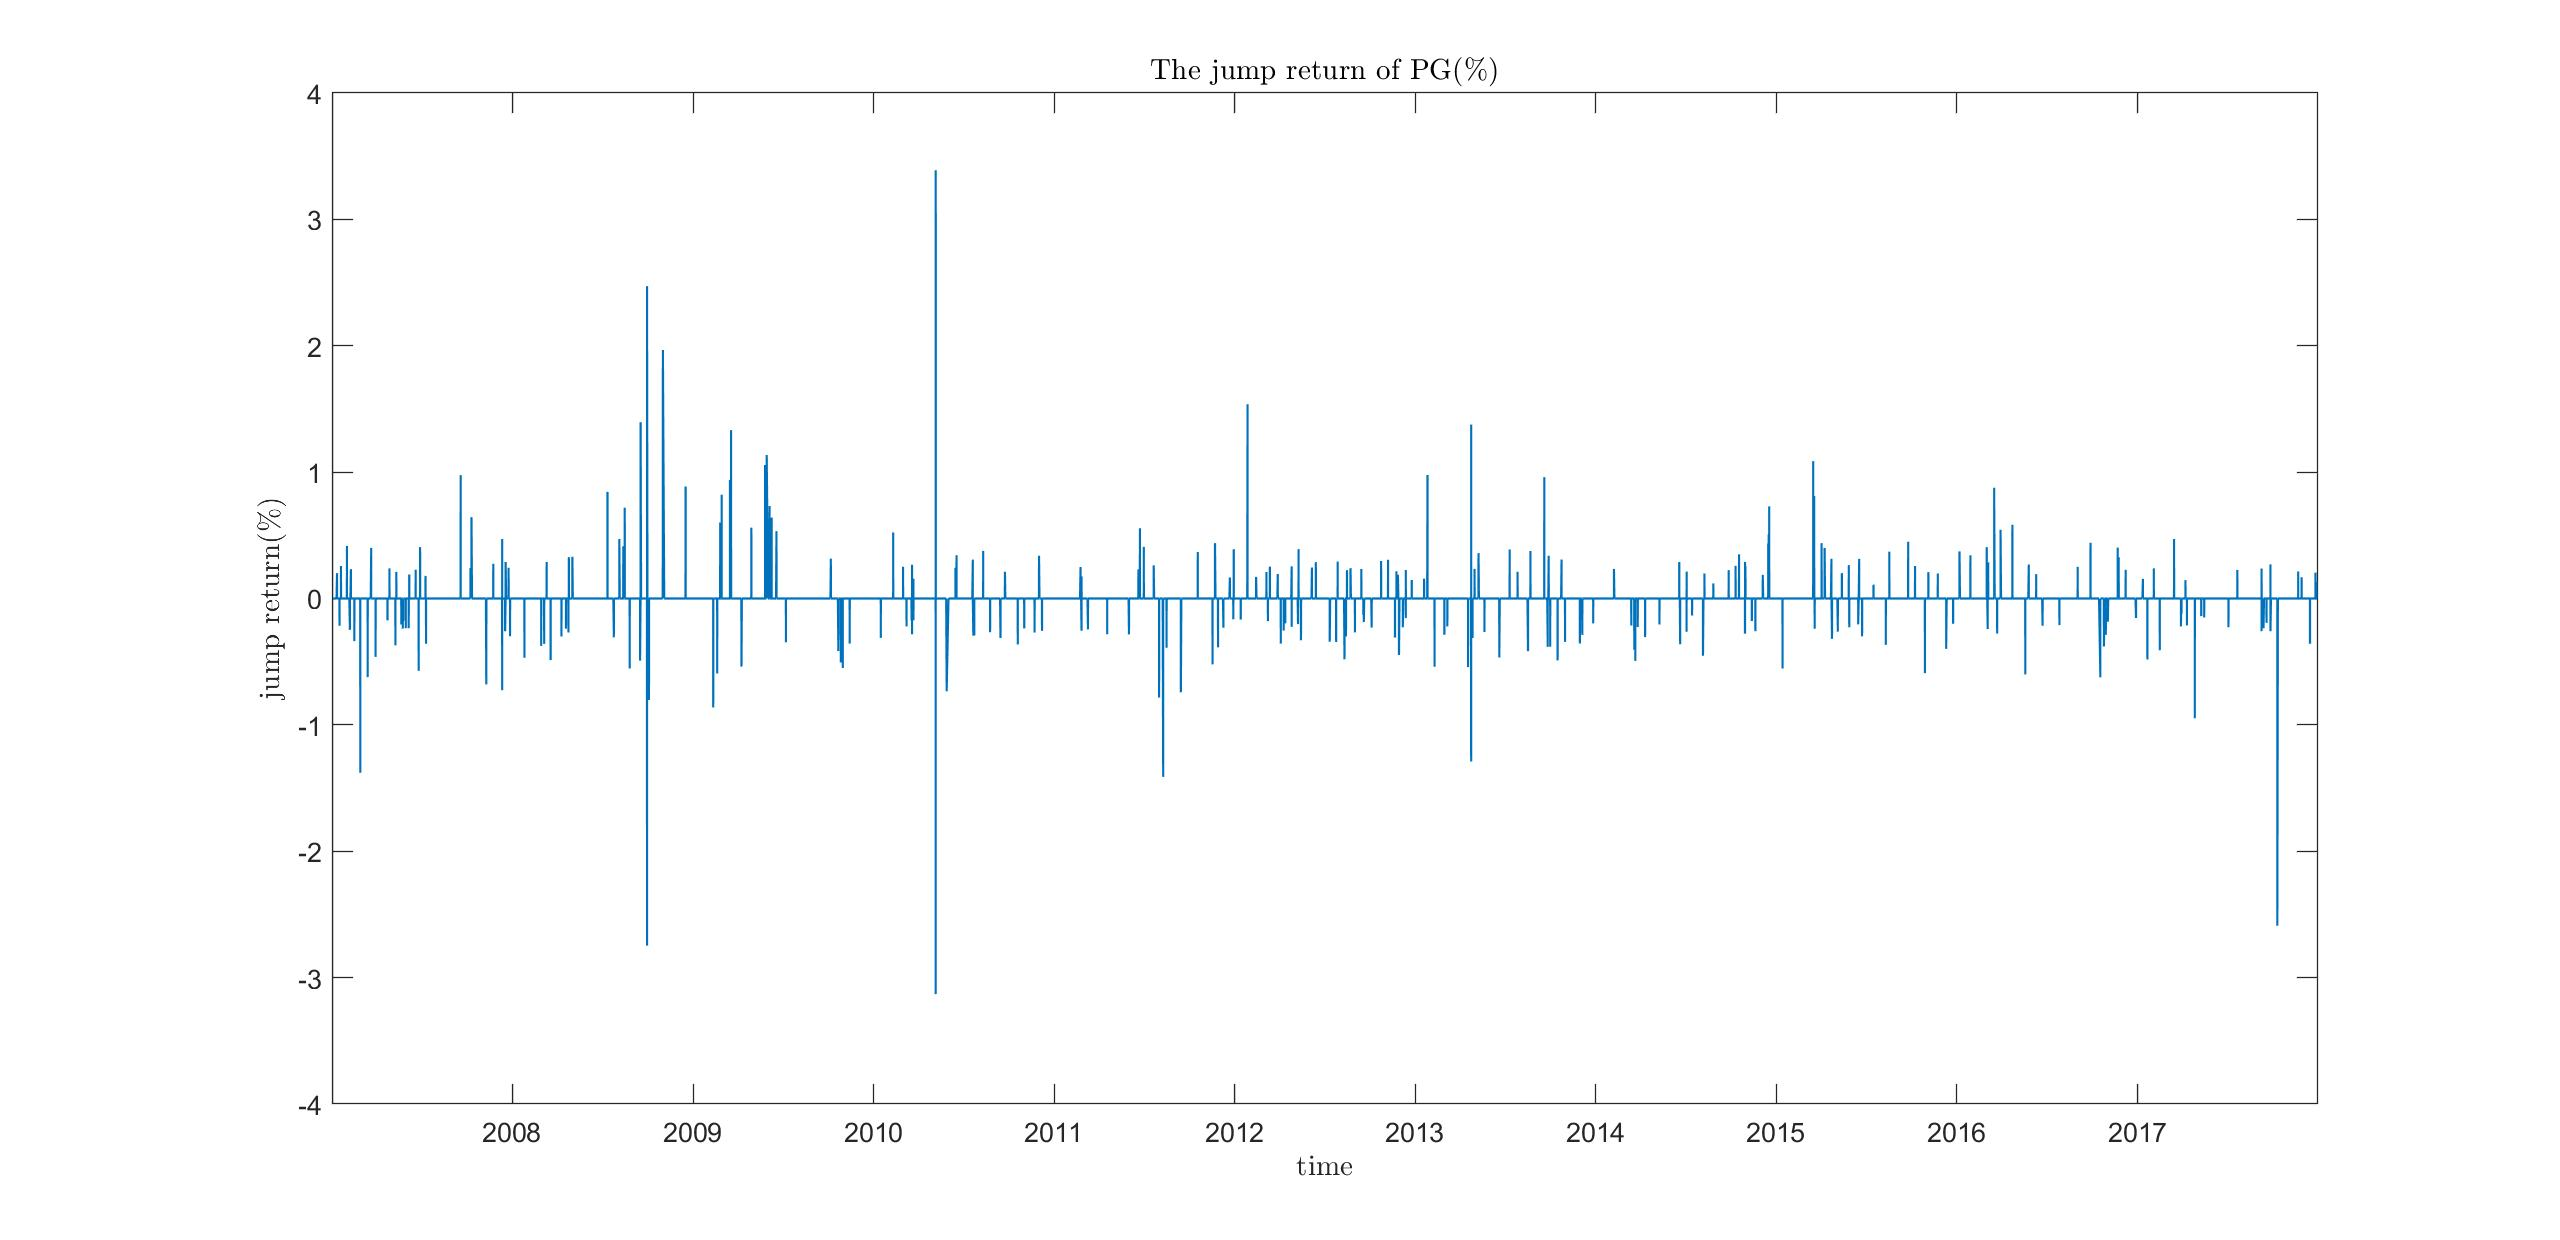
\includegraphics[width=3in]{figures/p3_ex1_c_d.jpg}
            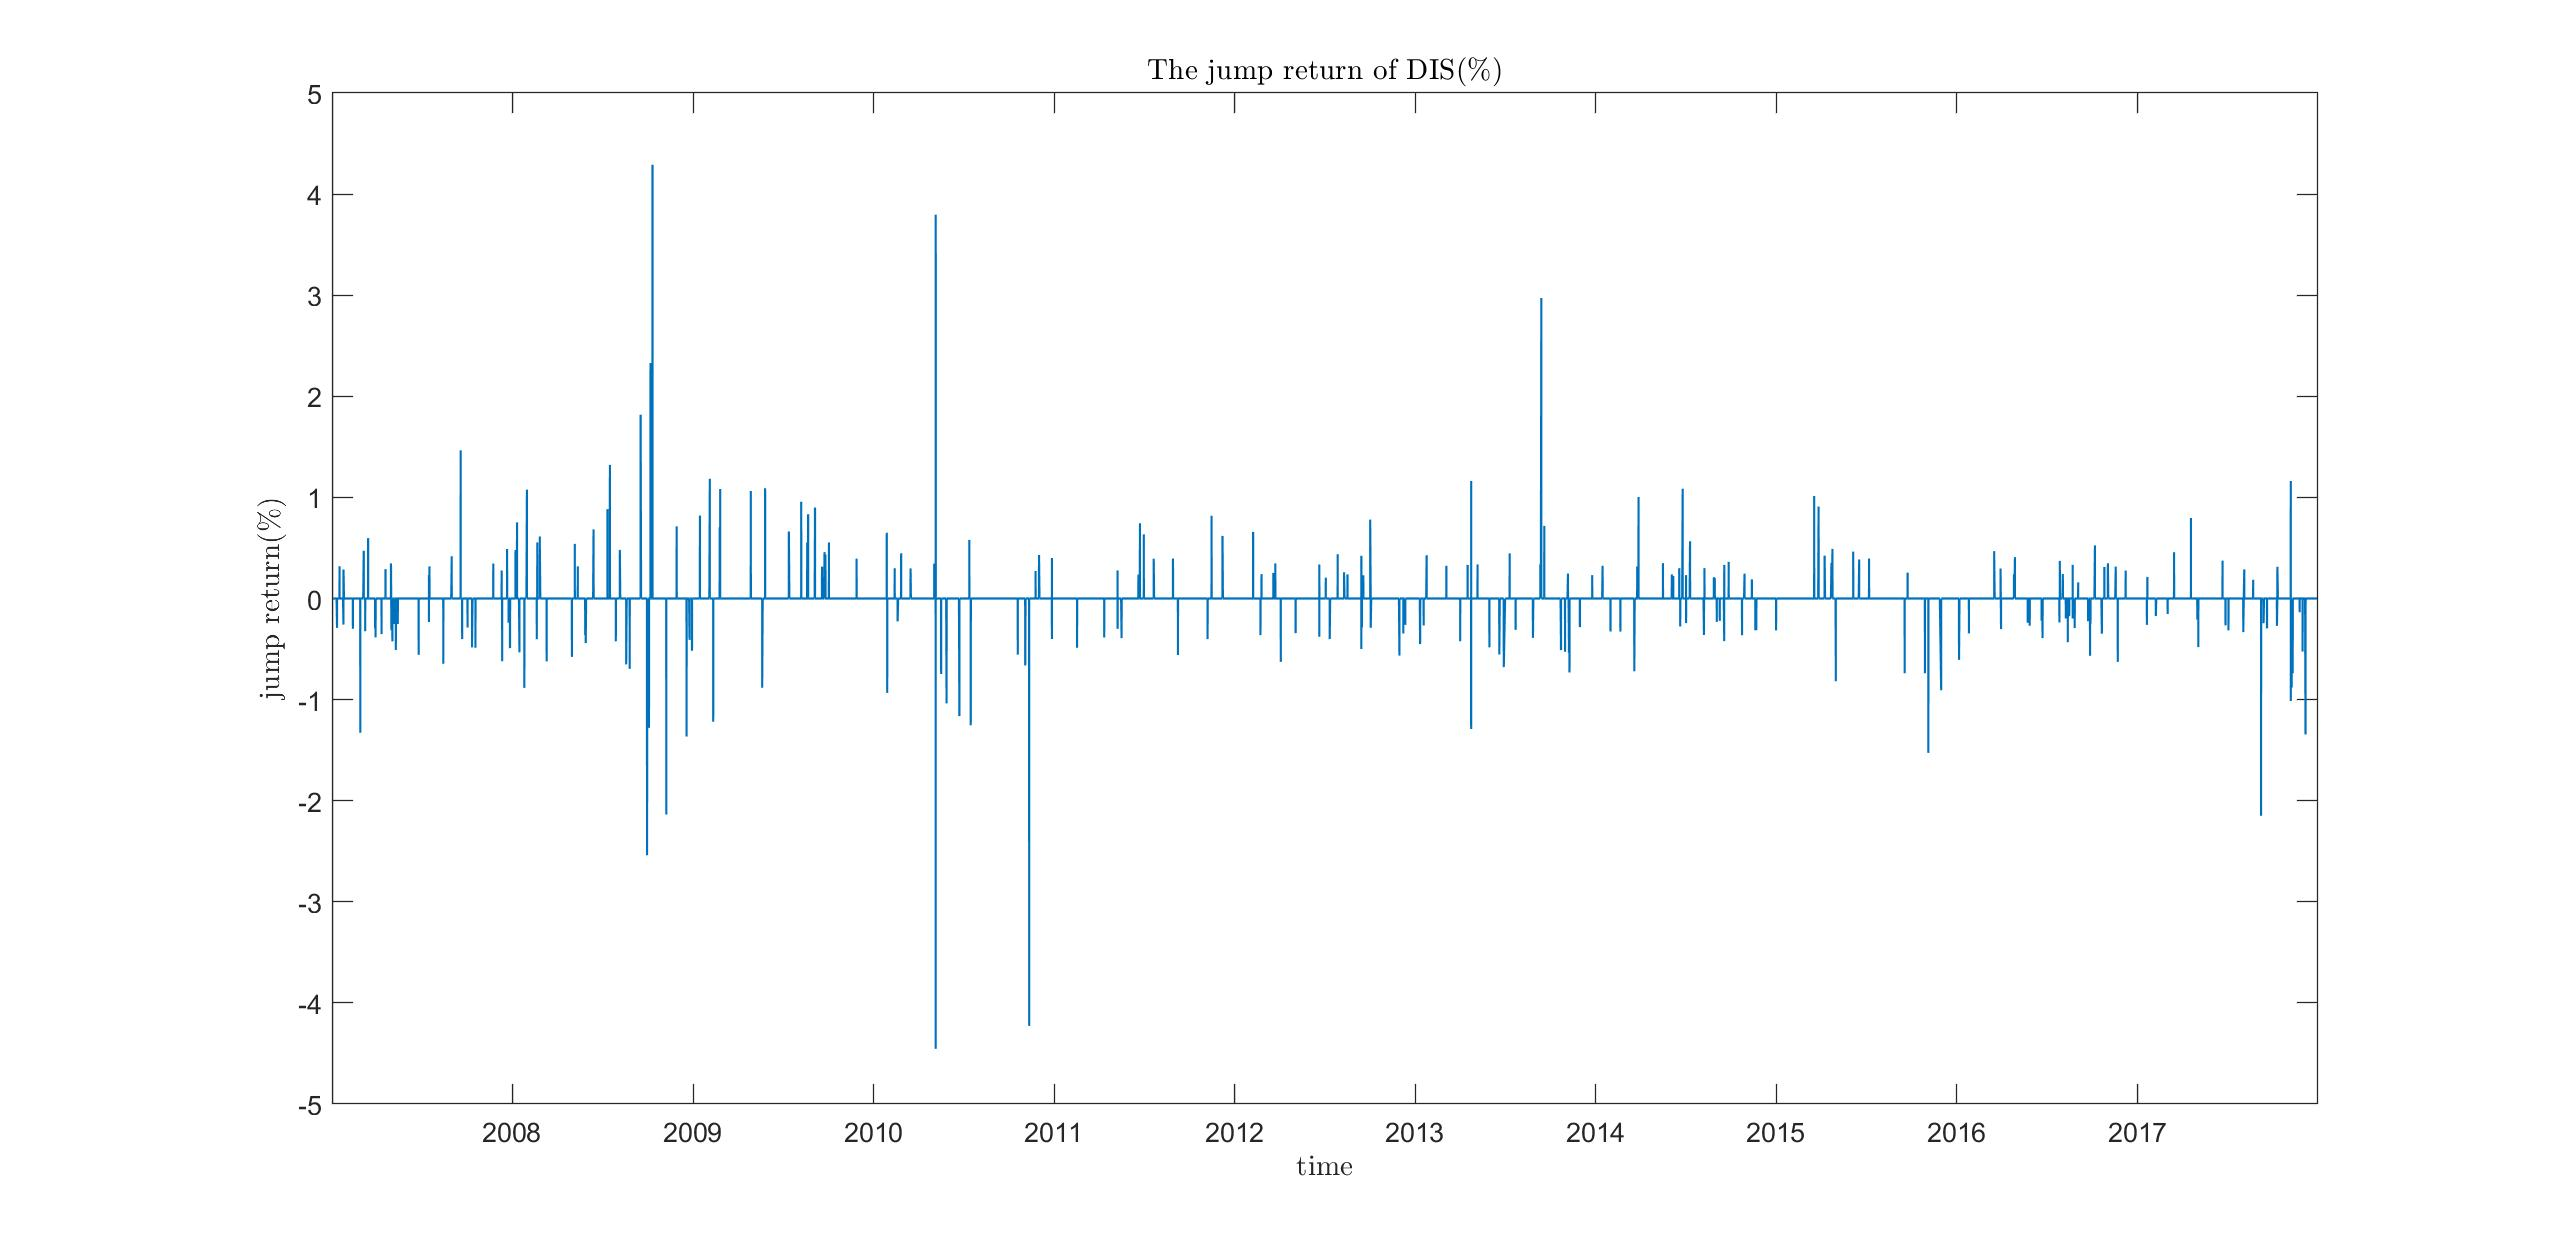
\includegraphics[width=3in]{figures/p3_ex1_c_d_DIS.jpg}
            \end{minipage}
            }
            \centering
            \caption{Diffusive returns and jump returns of PG and DIS}
\end{figure}

We can find the diffusive returns for both PG and DIS are moving around value 0, however, there are some abnormal values in these diffusive returns. For PG, it has three obvious abnormal diffusive returns: around the end of 2008, median 2010 and median 2015; for DIS, there are 5 obvious abnormal diffusive returns: around the begin of 2006, end of 2008, the end of 2011, median 2012 and median 2015. These abnormal returns show that our data may probably exist outliers. \\

As for the jump returns, we find that the jumps return has smaller sample number than diffusive returns. Same as diffusive returns, we can observe that the jump returns move around 0 value and we can not find significant trend of jump returns deviate from zero. The frequency of large returns are higher in jump returns than diffusive returns. Without doing some statistic works, We can not tell which jump type (positive jump or negative jump) happens more frequently just through these figures.\\


The \textbf{MATLAB} code:
   \lstinputlisting{functions/bipower_var_day.m}
   \lstinputlisting{functions/cut_off.m}
   \lstinputlisting{functions/c_d_log_returns.m}

%-------D-----------
\item The number of jumps from 2007 to 2017 for PG is [38, 24,21,29,22,44,28,28,25,24,27] and total 310. 
The number of jumps each for PG is [37,33,20,21,14,24,26,32,15,32,27] and total 281 times.\\
\begin{figure}[H]
           \subfigure{
           \begin{minipage}[l]{1\linewidth}
           \centering
            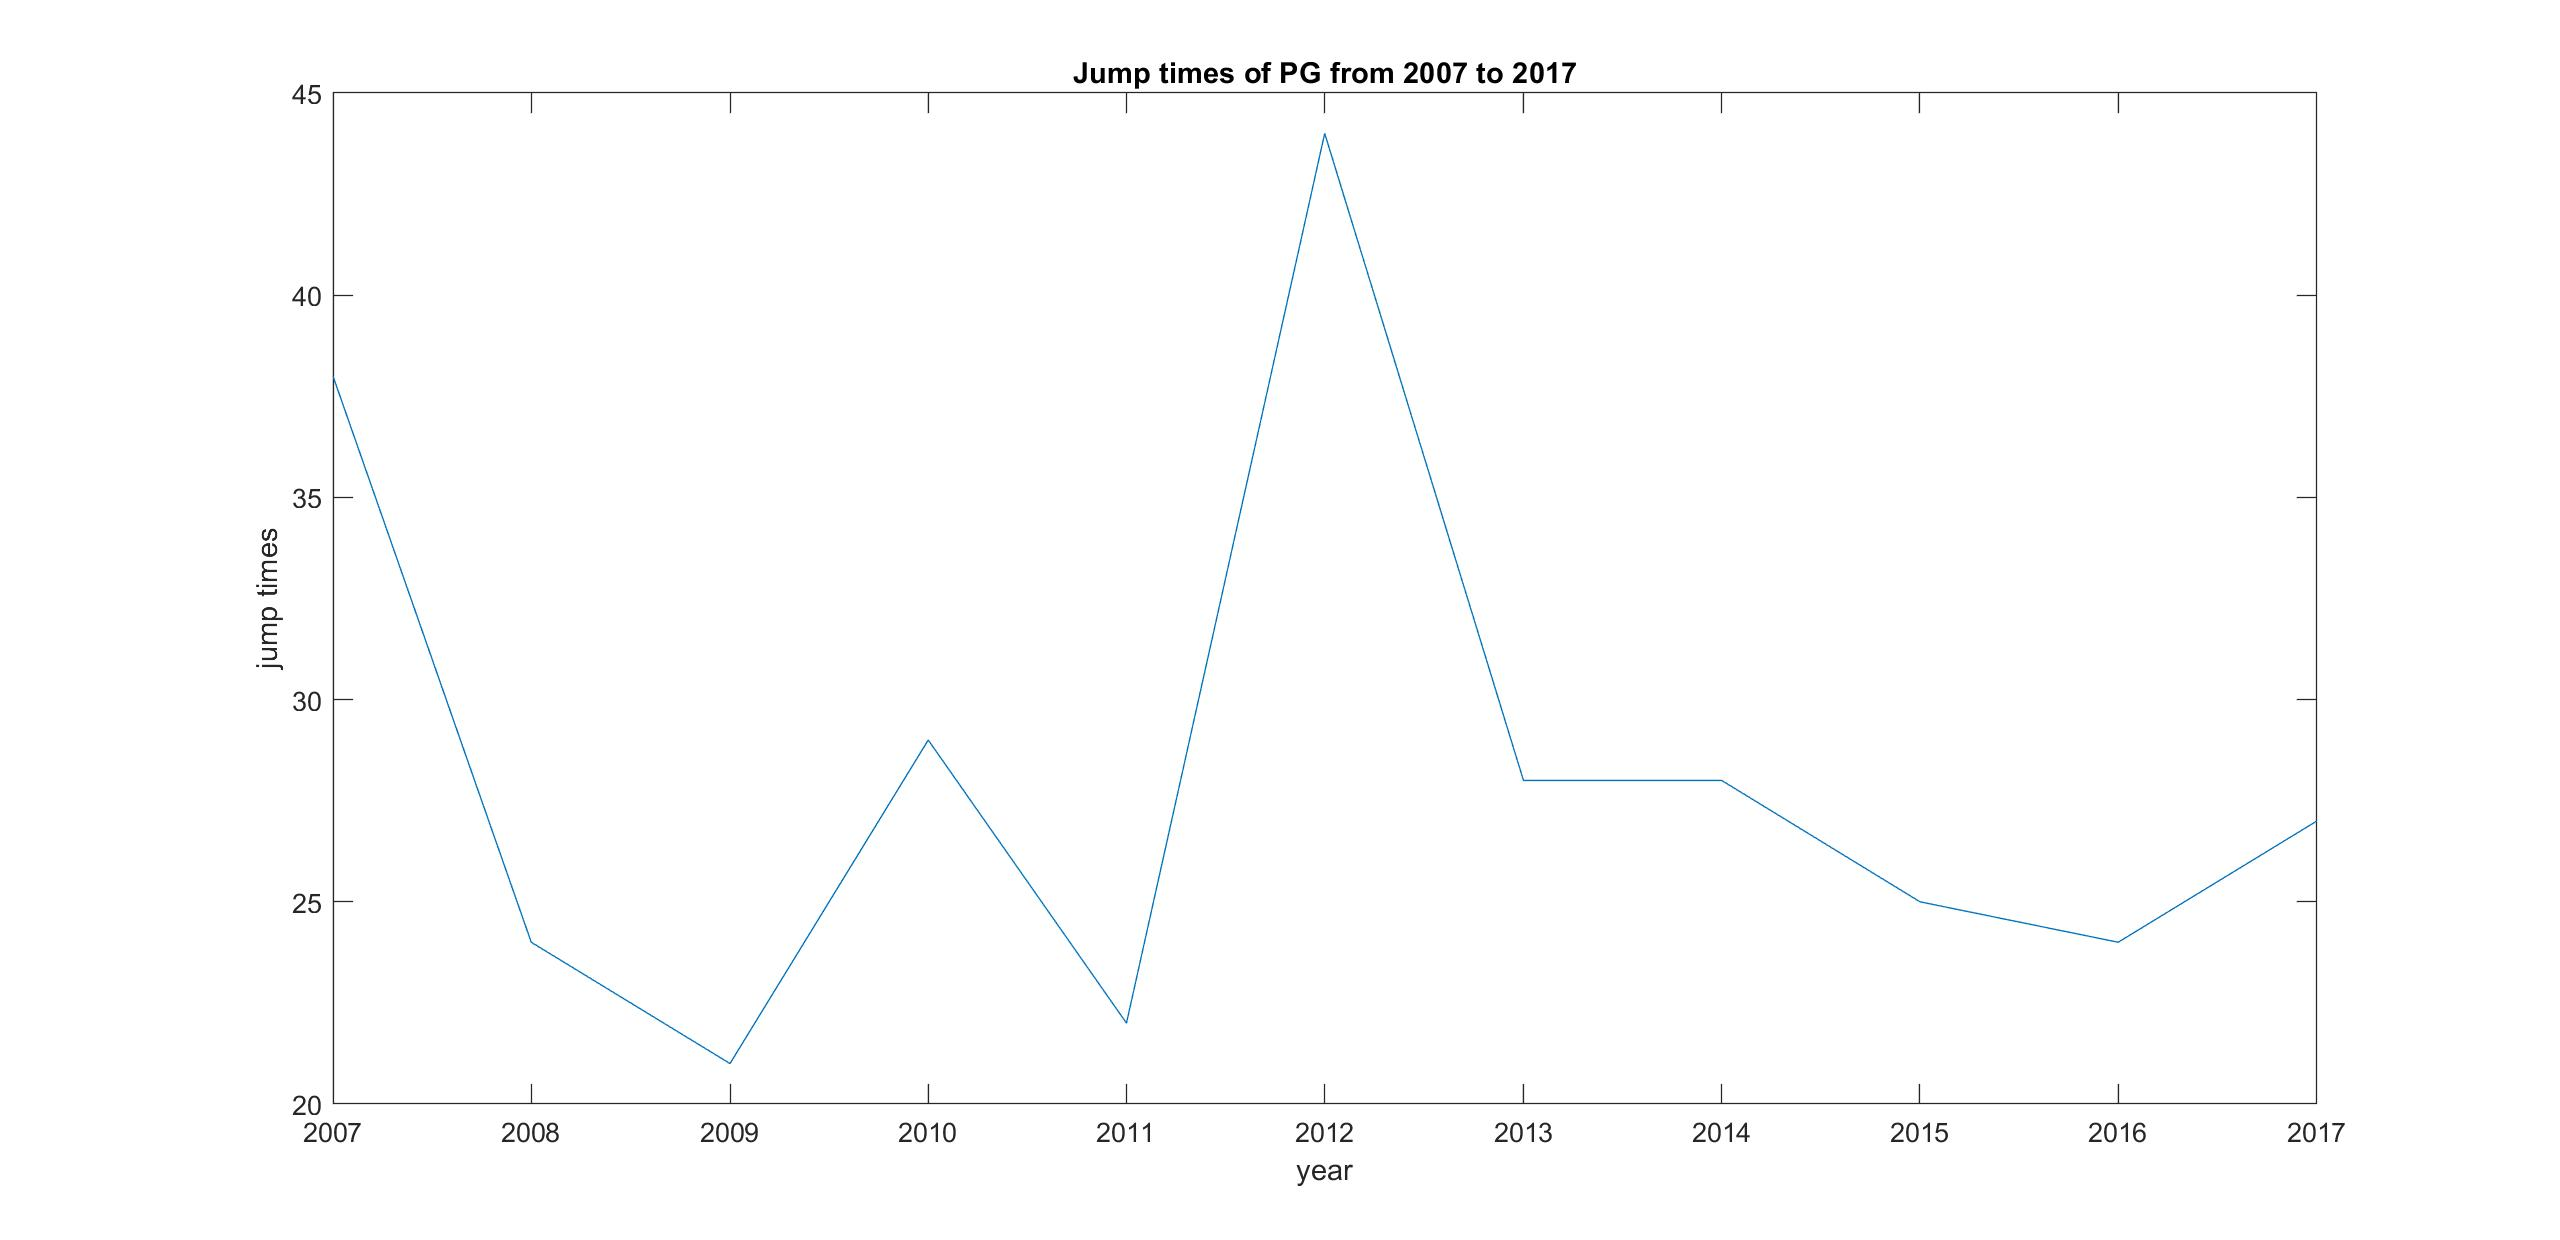
\includegraphics[width=3in]{figures/p3_ex1_d.jpg}
            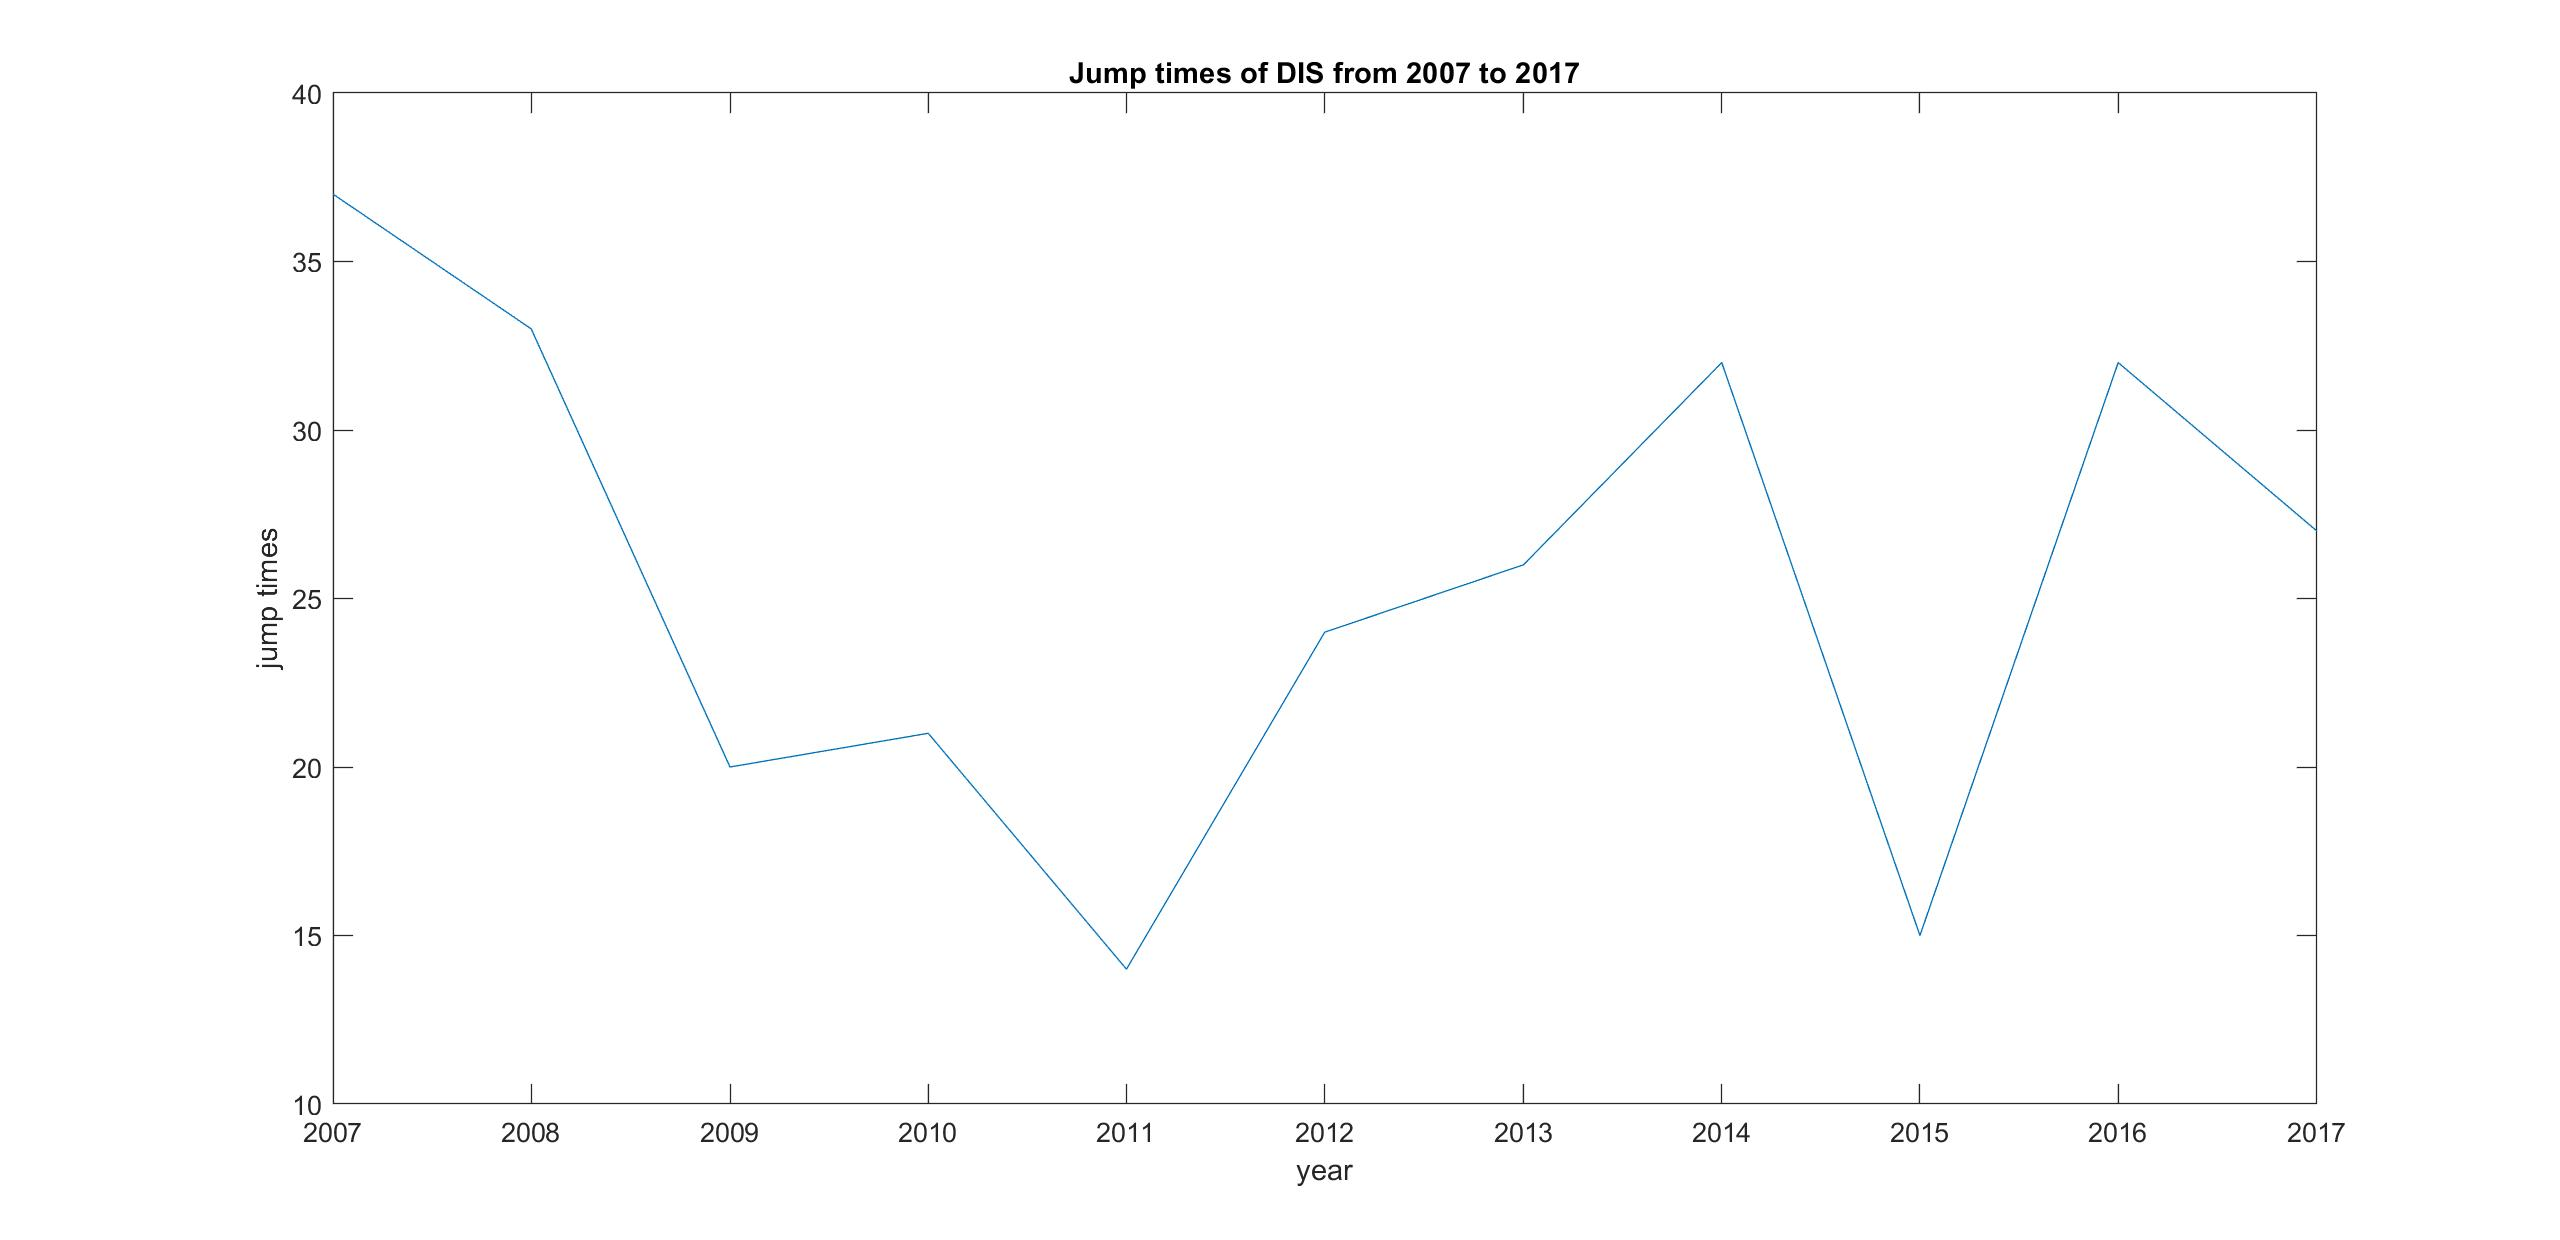
\includegraphics[width=3in]{figures/p3_ex1_d_DIS.jpg}
            \end{minipage}
            }
            \centering
            \caption{Jump times each year(from 2007 to 2017)}
\end{figure}
      As we can notice from this figure, there are more jumps in the year when  there are crisis, say 2007, 2012 and 2015. From the jump returns figures in part C, we can find that there usually more jumps around the end of year.\\
      
   
%-------E-----------
\item The follows are the histogram figures of PG and DIS' diffusive returns and non-zero jump returns.
\begin{figure}[H]
           \subfigure{
           \begin{minipage}[l]{1\linewidth}
           \centering
            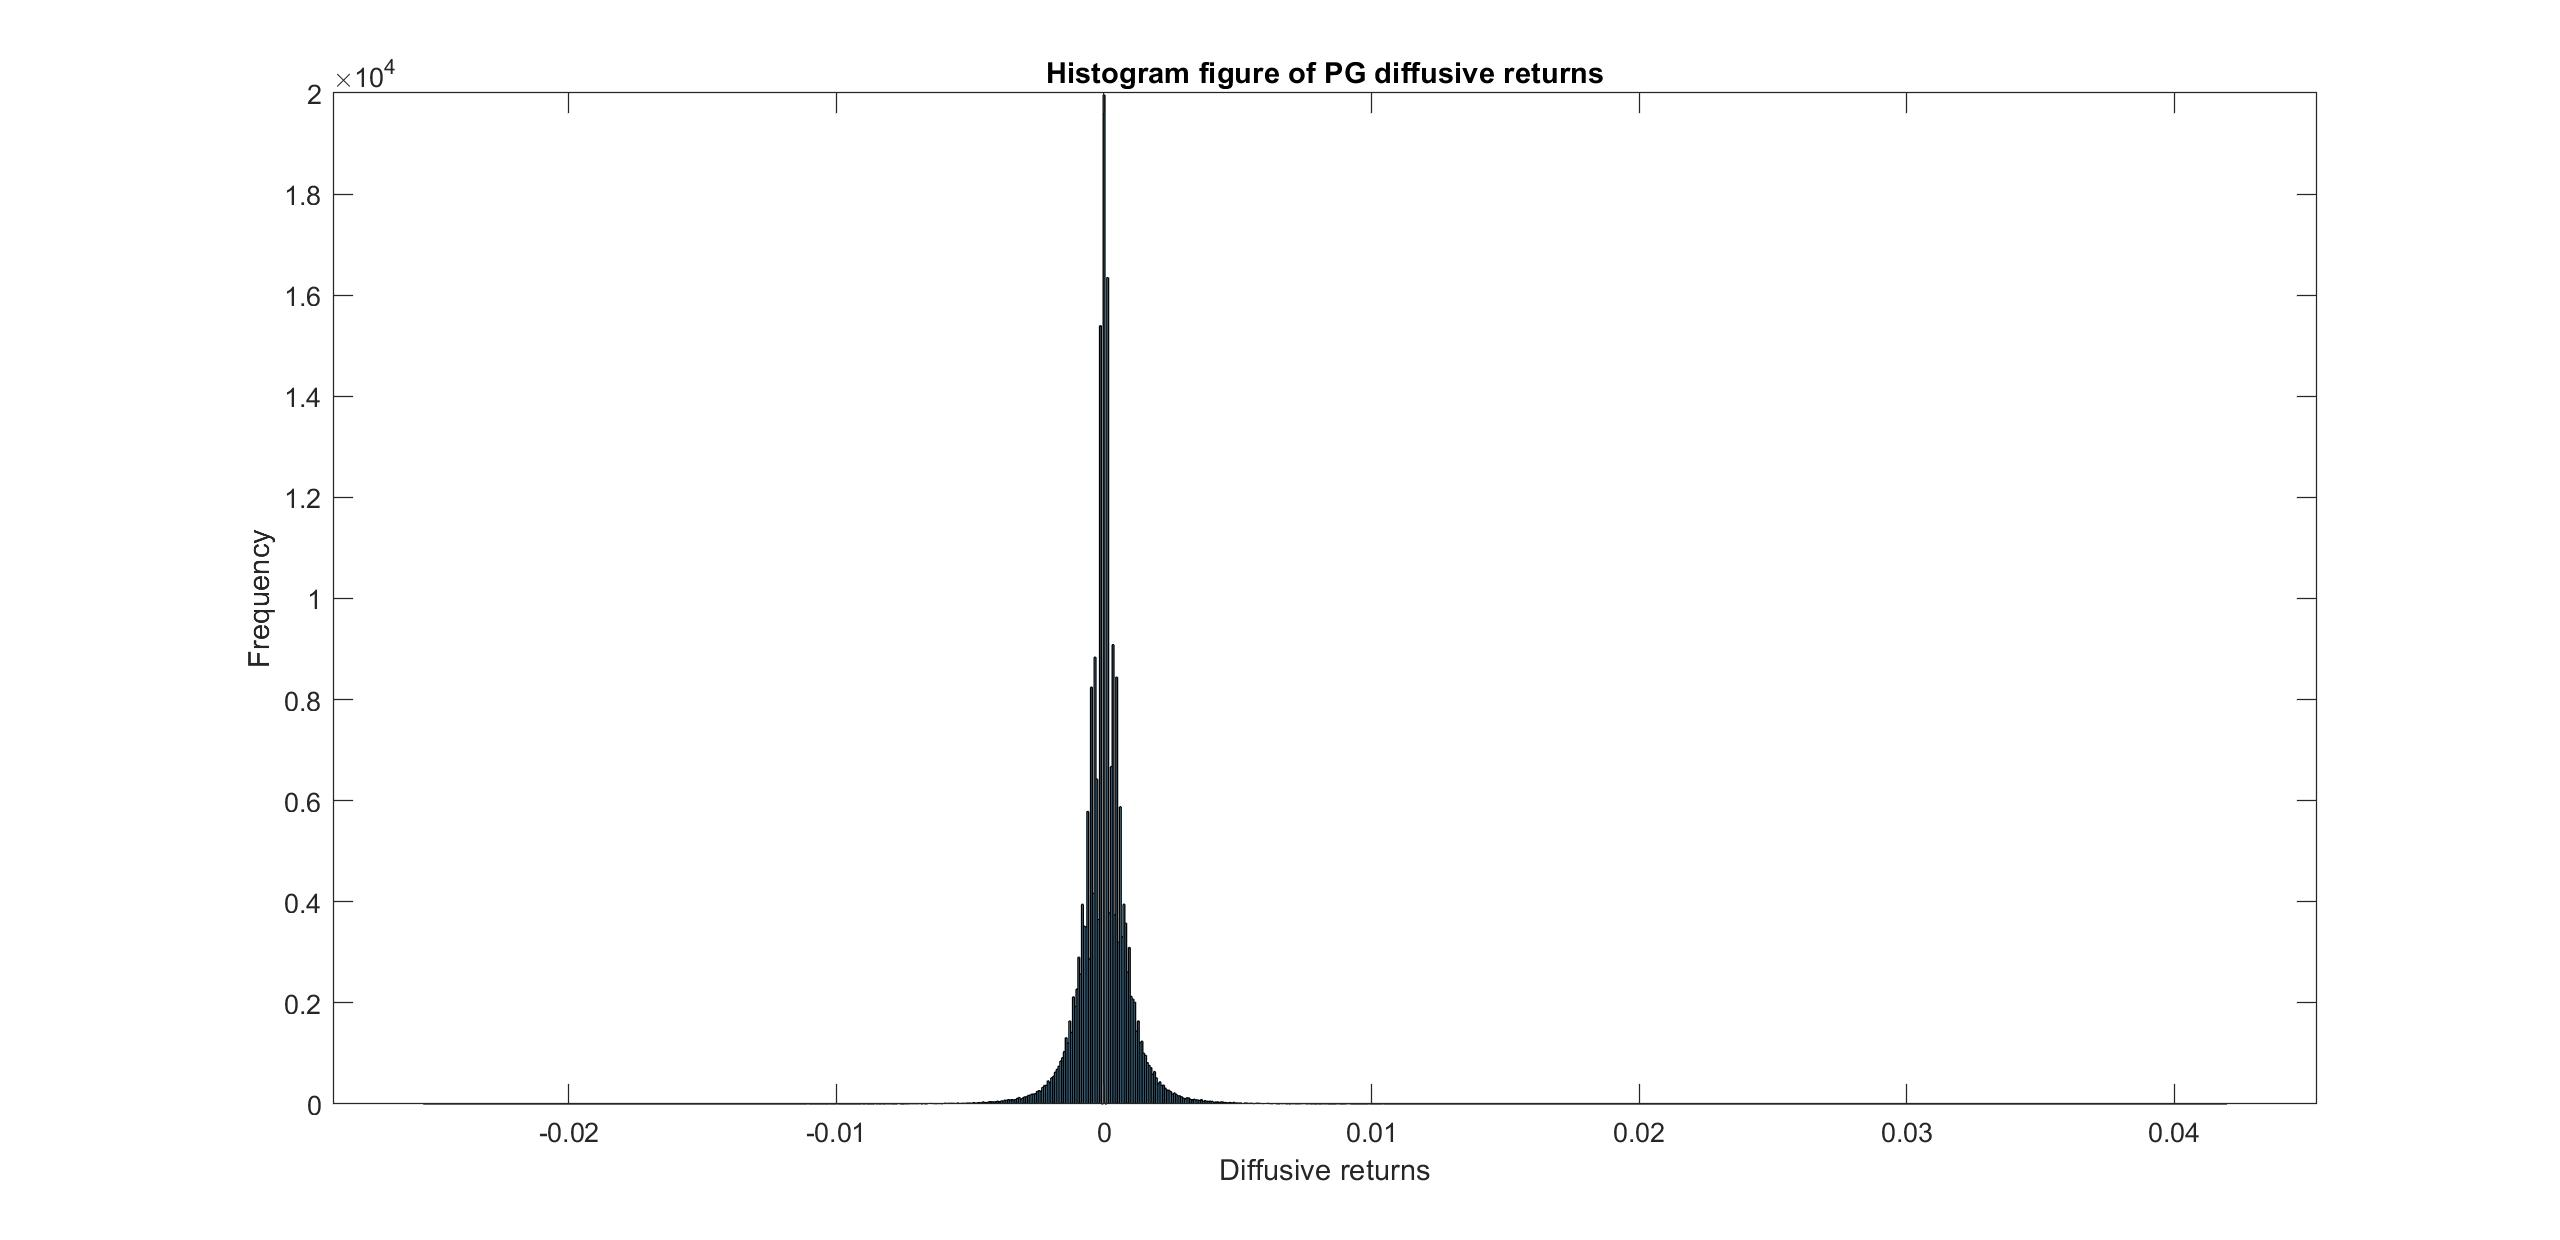
\includegraphics[width=3in]{figures/p3_ex1_e_1.jpg}
            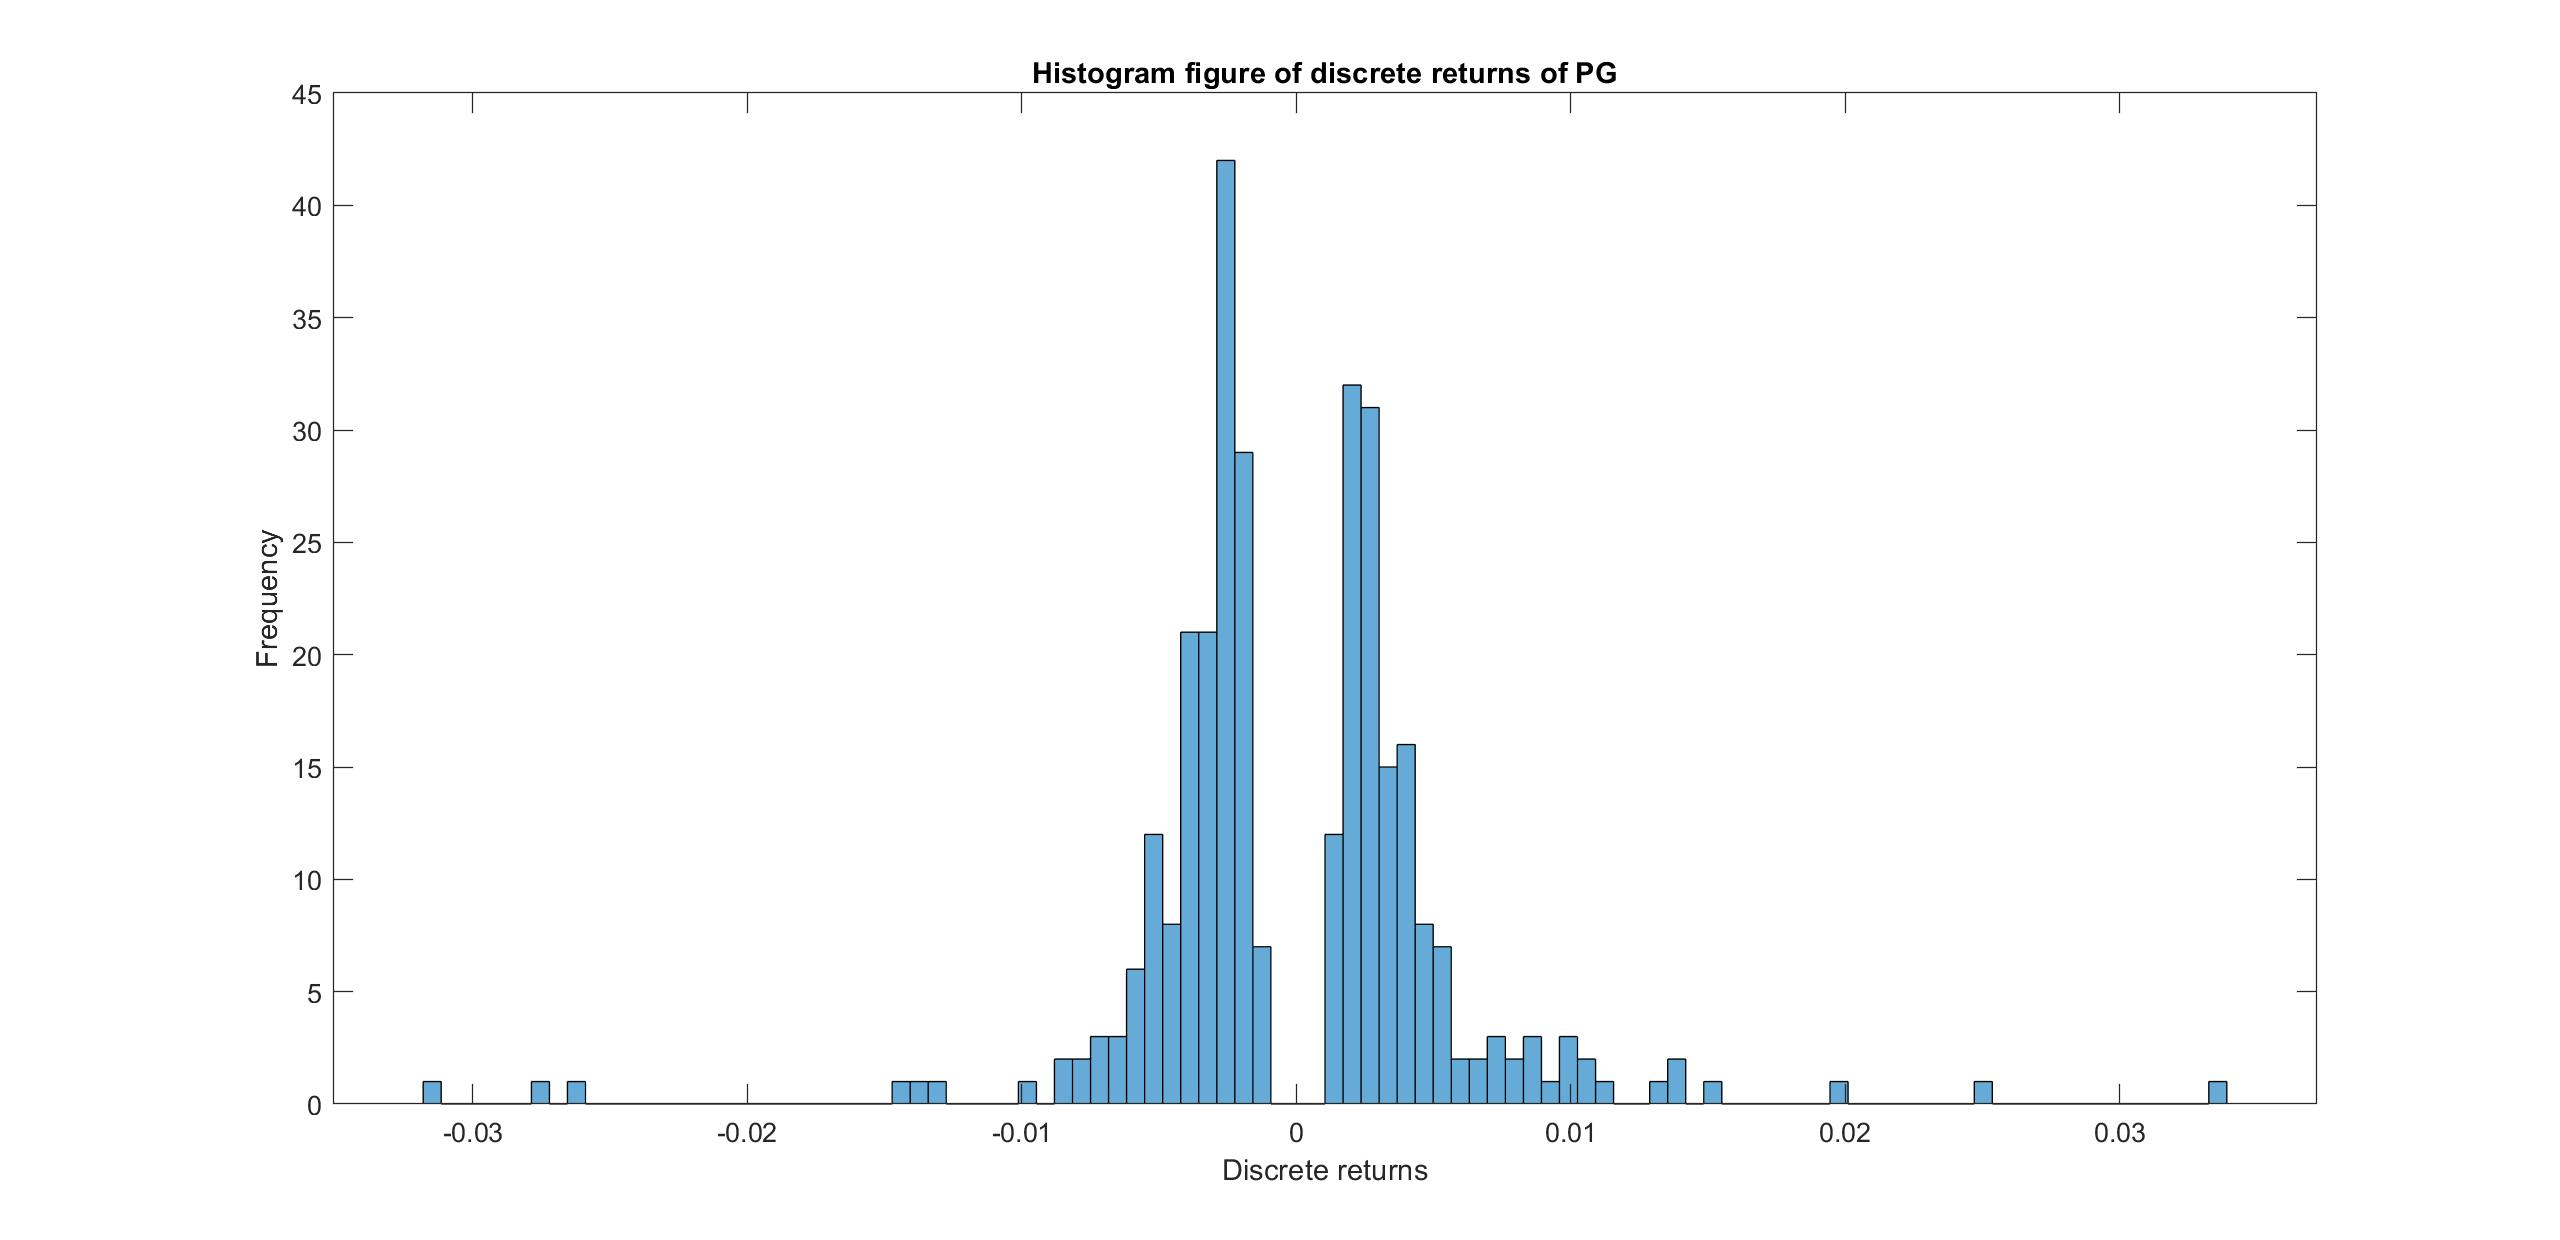
\includegraphics[width=3in]{figures/p3_ex1_e_3.jpg}
            \end{minipage}
            }
             \subfigure{
           \begin{minipage}[l]{1\linewidth}
           \centering
            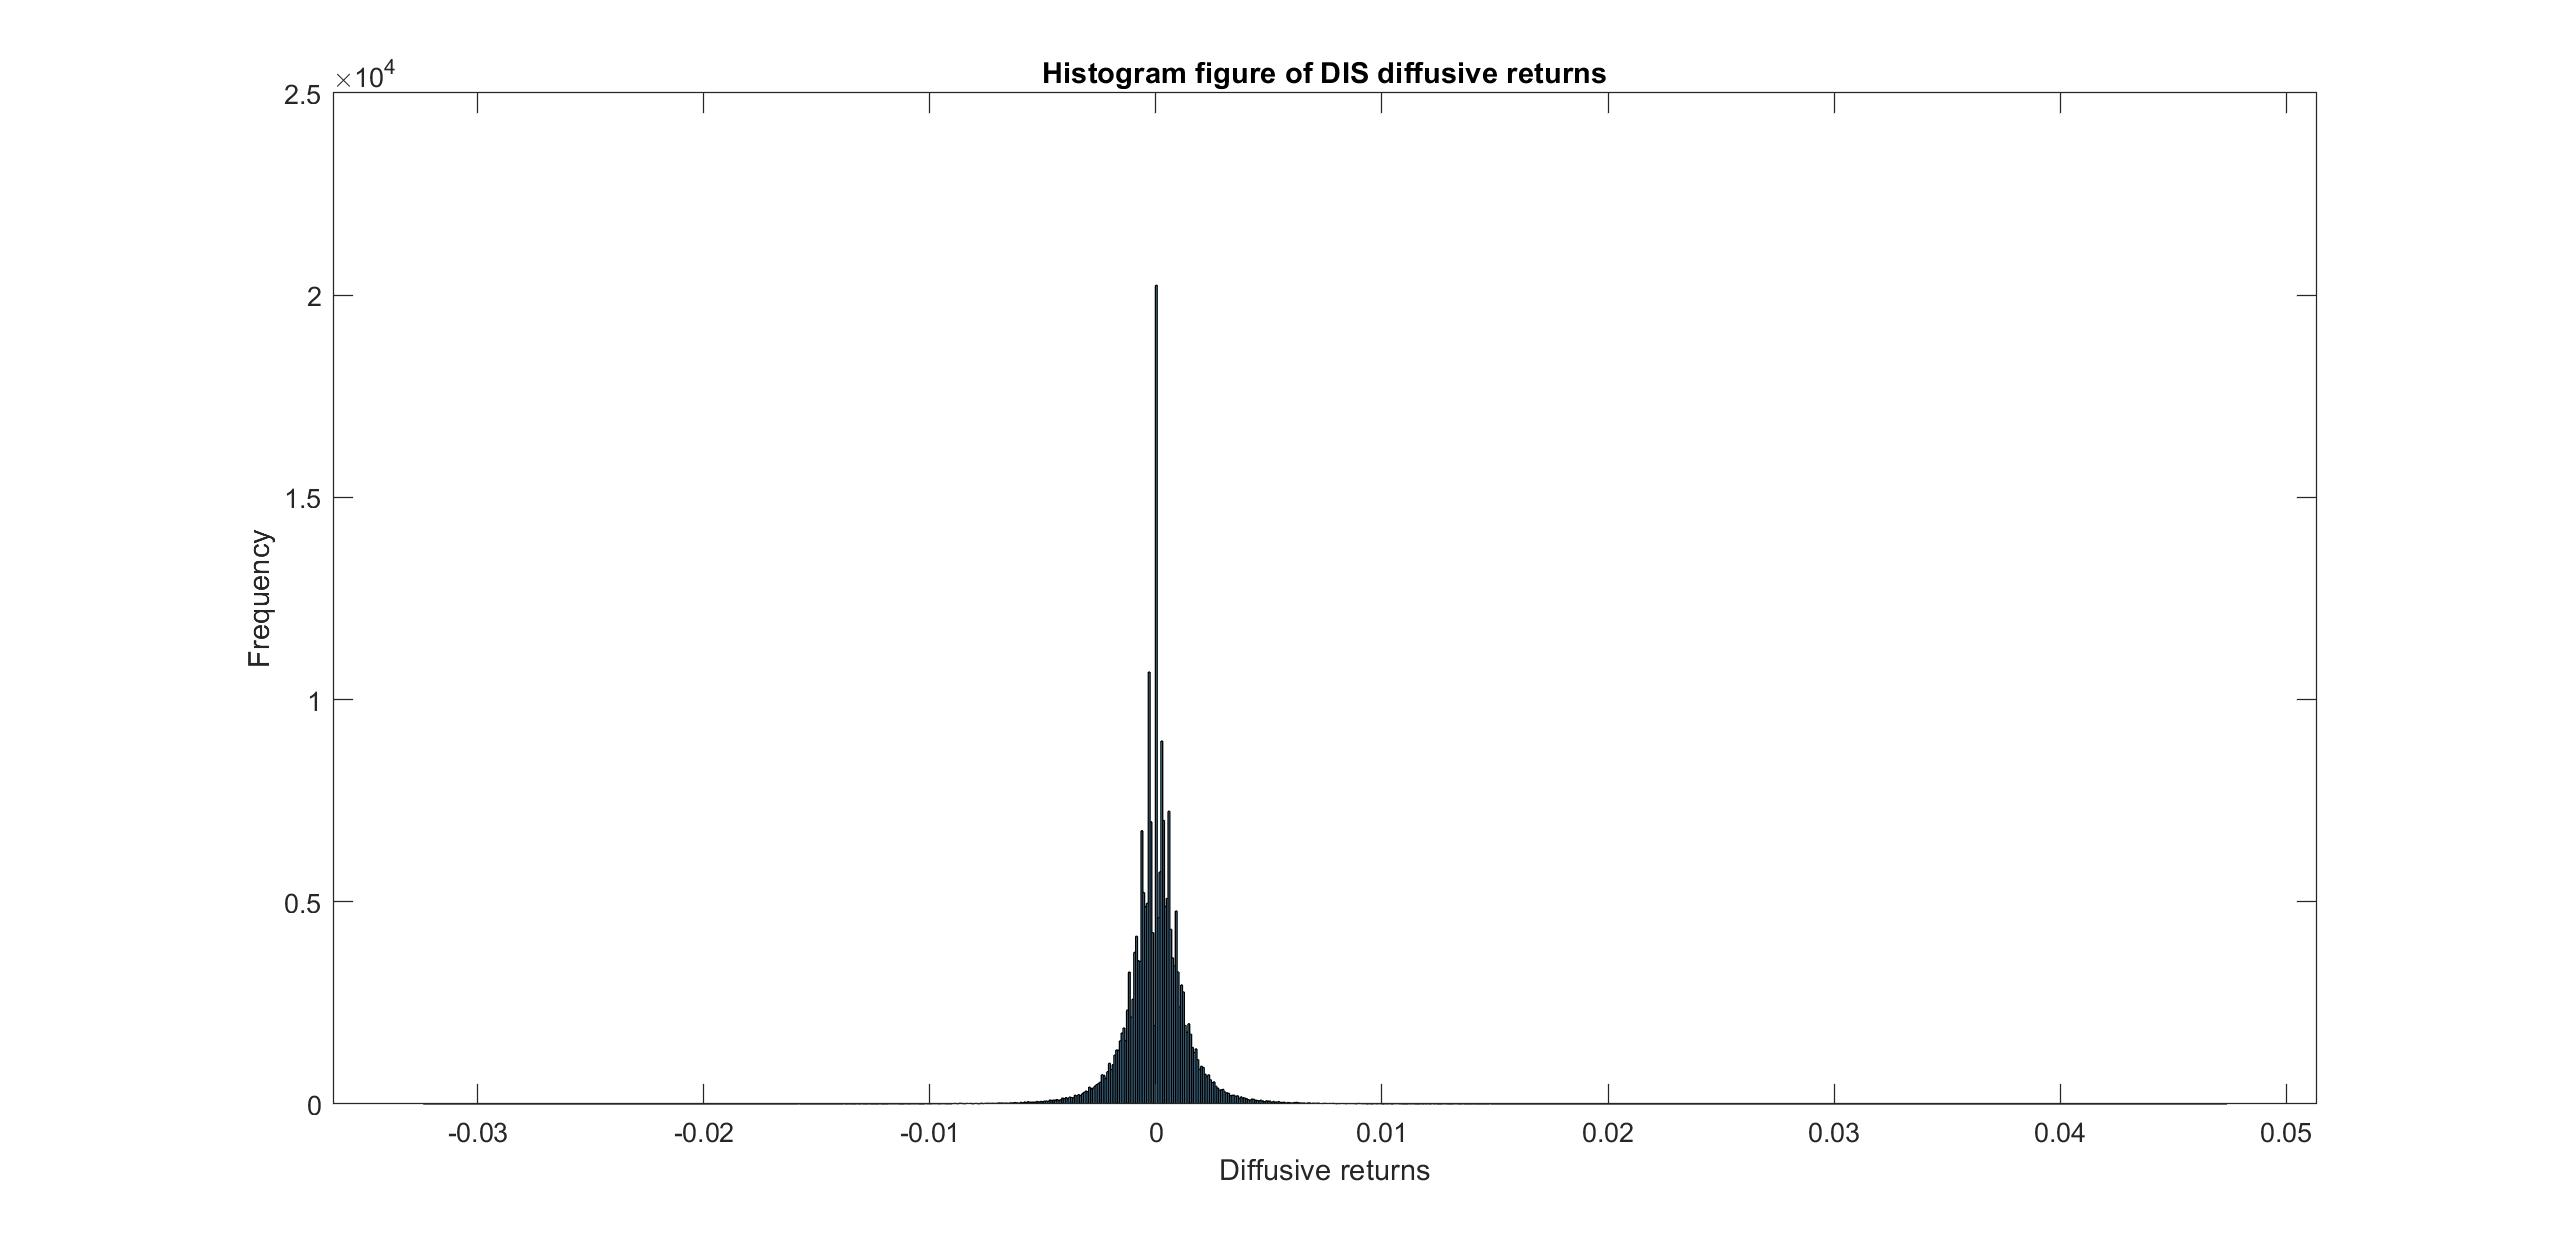
\includegraphics[width=3in]{figures/p3_ex1_e_1_DIS.jpg}
            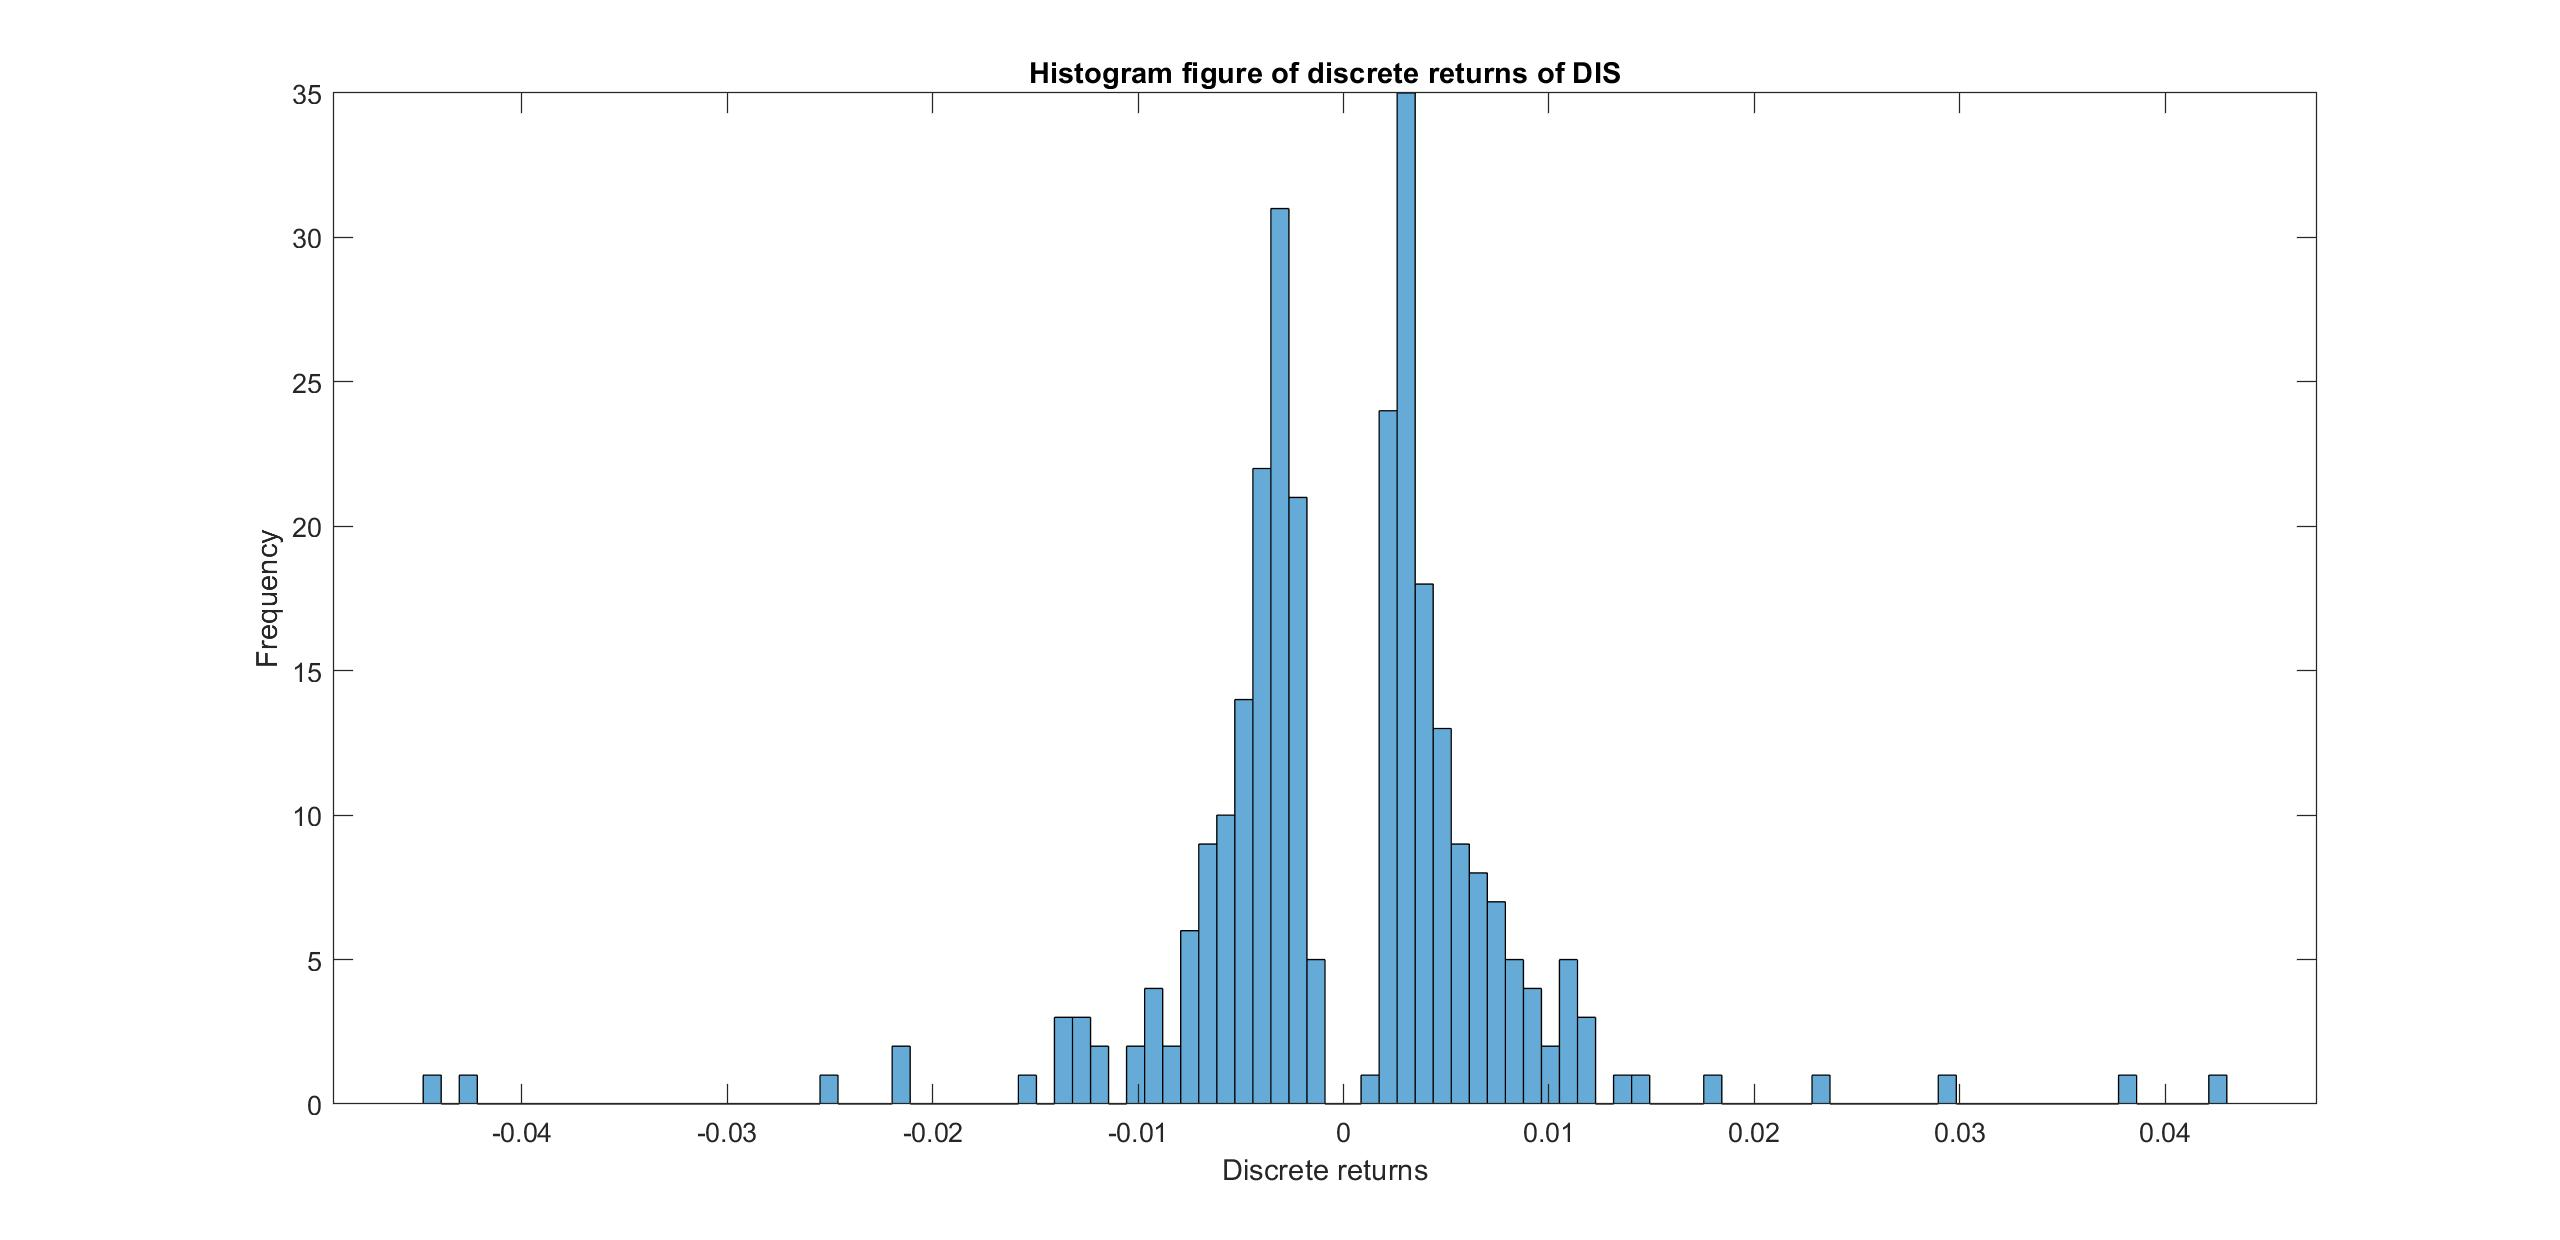
\includegraphics[width=3in]{figures/p3_ex1_e_3_DIS.jpg}
            \end{minipage}
            }
            \centering
            \caption{Histograms of diffusive returns and jump returns for PG and DIS}
\end{figure}

We can see from the figures that the distribution of diffusive returns for PG and DIS are very similar to normal distribution with mean equal to zero. In order to catch the characteristics of its distribution, we delete the zero value when plot the figures.As we can see from the figure, the jump returns distribution may have two peaks and skew to the left. 

It is hard to tell the distribution of jump returns without deleting zero values in our sample. If there must be a distribution of total jump returns(include bunch of zeros), the distribution may have mean =0 and volatility very close to 0. Since the non zeros jumps returns just take up 0.15\% in total sample, the distribution type will mainly depend on large zero part. 
\\

%-------G-----------
\item Since it makes no sense to discuss about the distribution of jump returns with bunch of zero samples, so here just do distribution estimation for non-zero jump returns. The follows are the figures of estimated p.d.f. of diffusive returns and non-zero jump returns of PG and DIS.
\begin{figure}[H]
           \subfigure{
           \begin{minipage}[l]{1\linewidth}
           \centering
            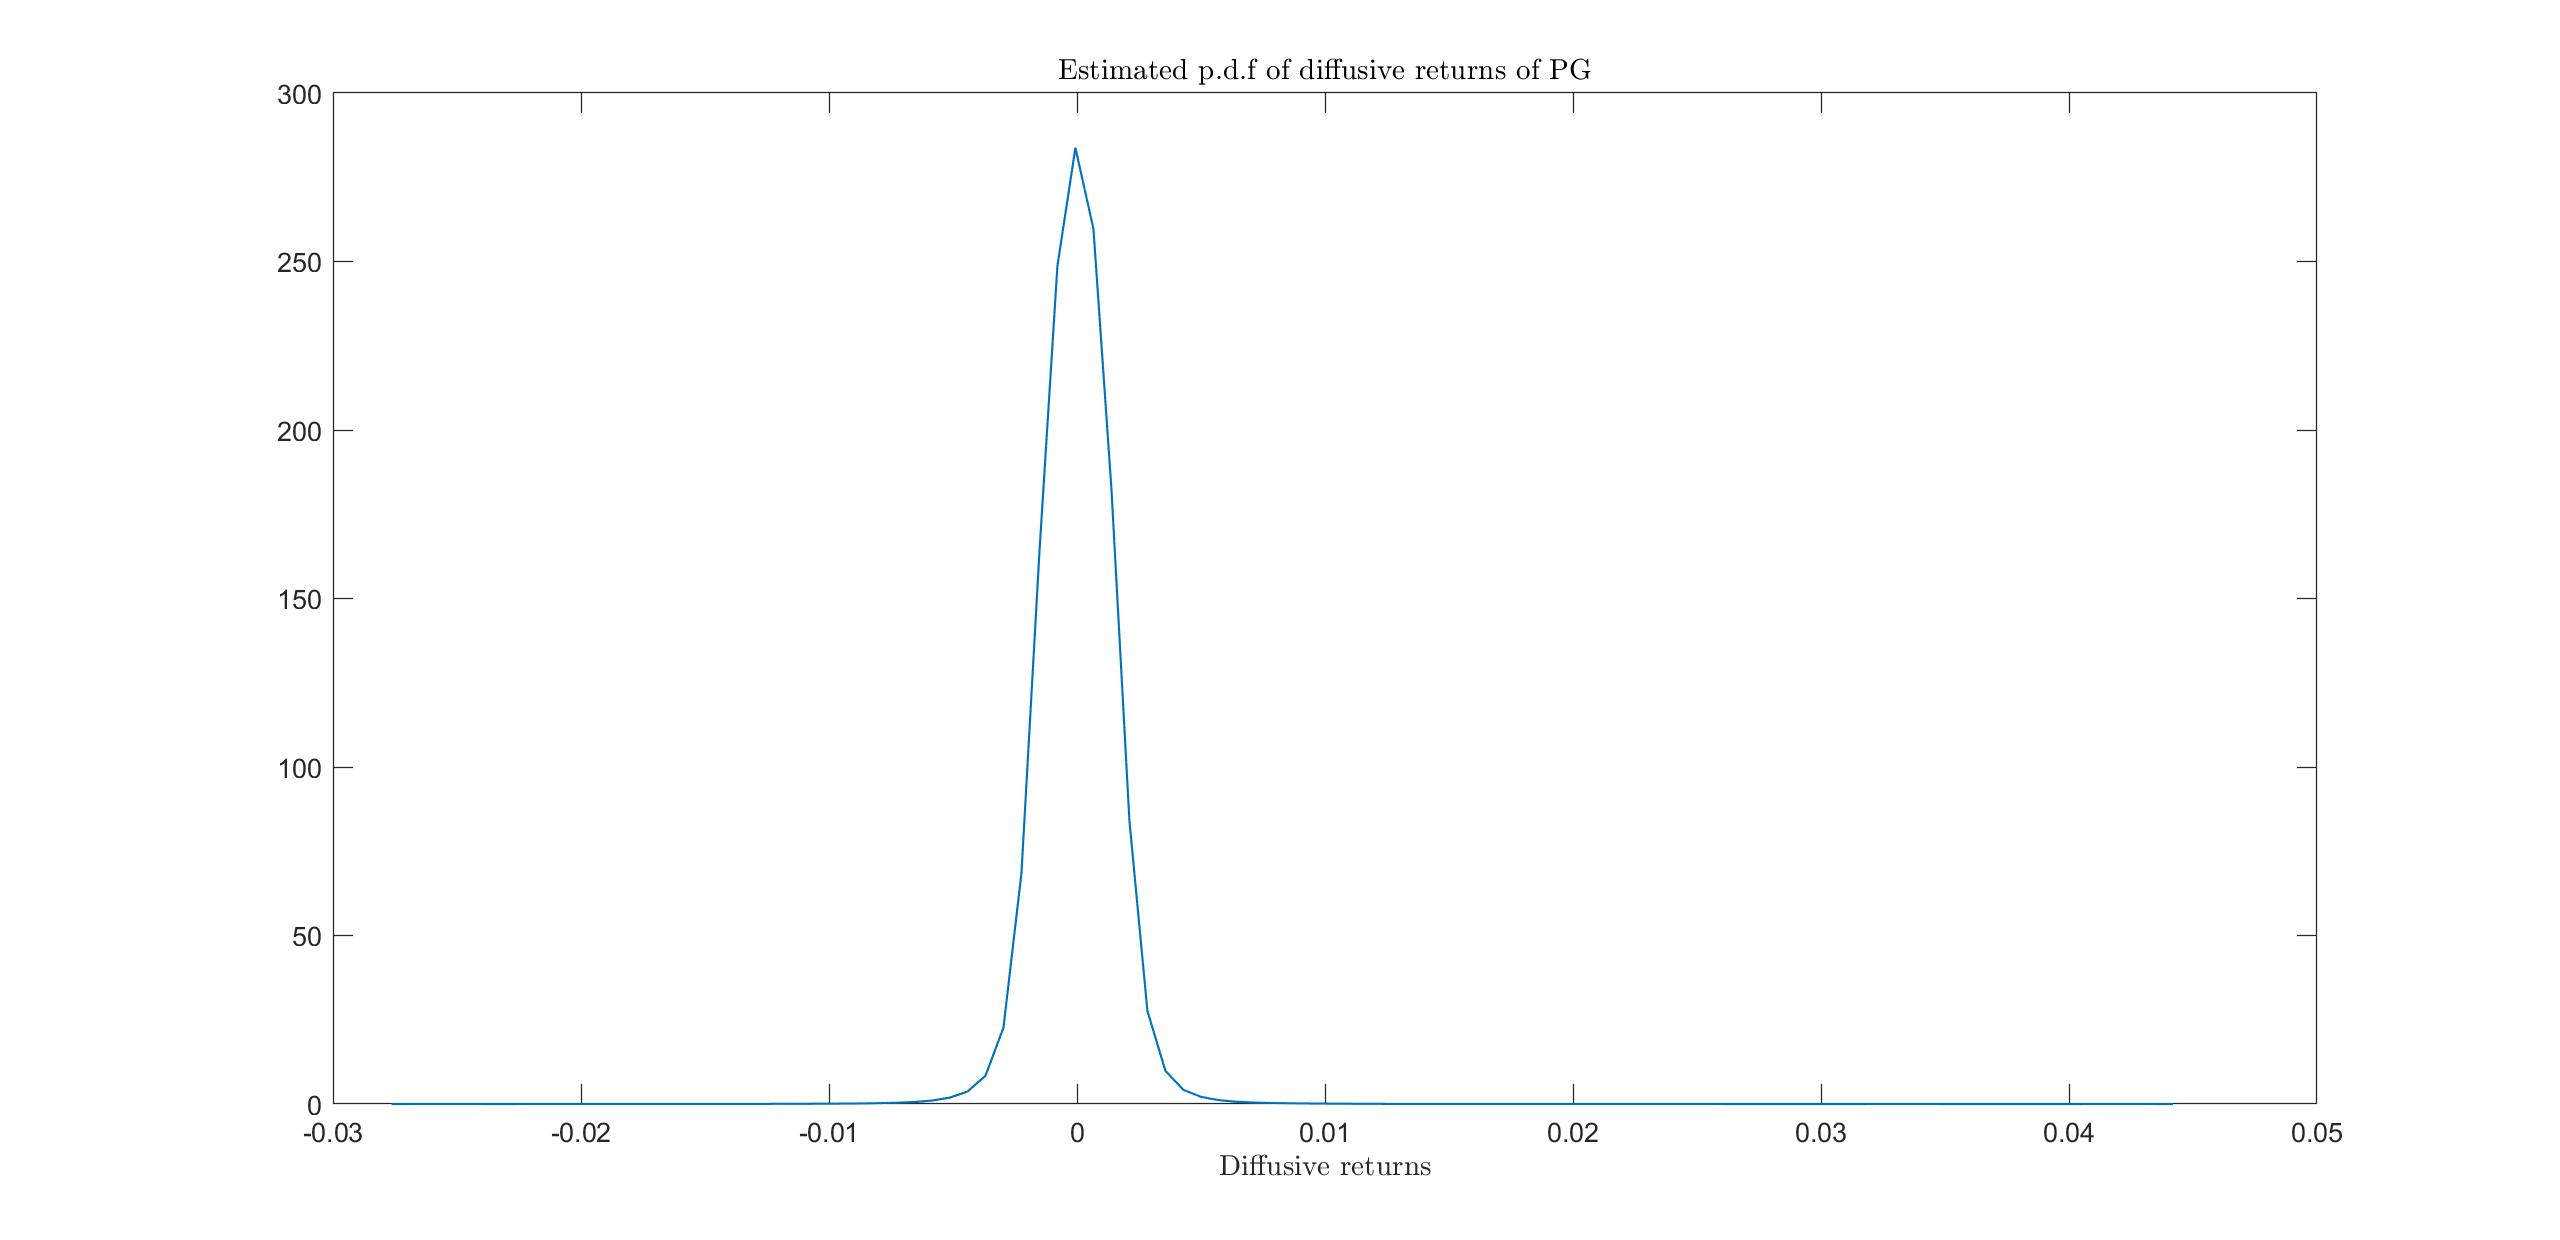
\includegraphics[width=3in]{figures/p3_ex1_g_c.jpg}
            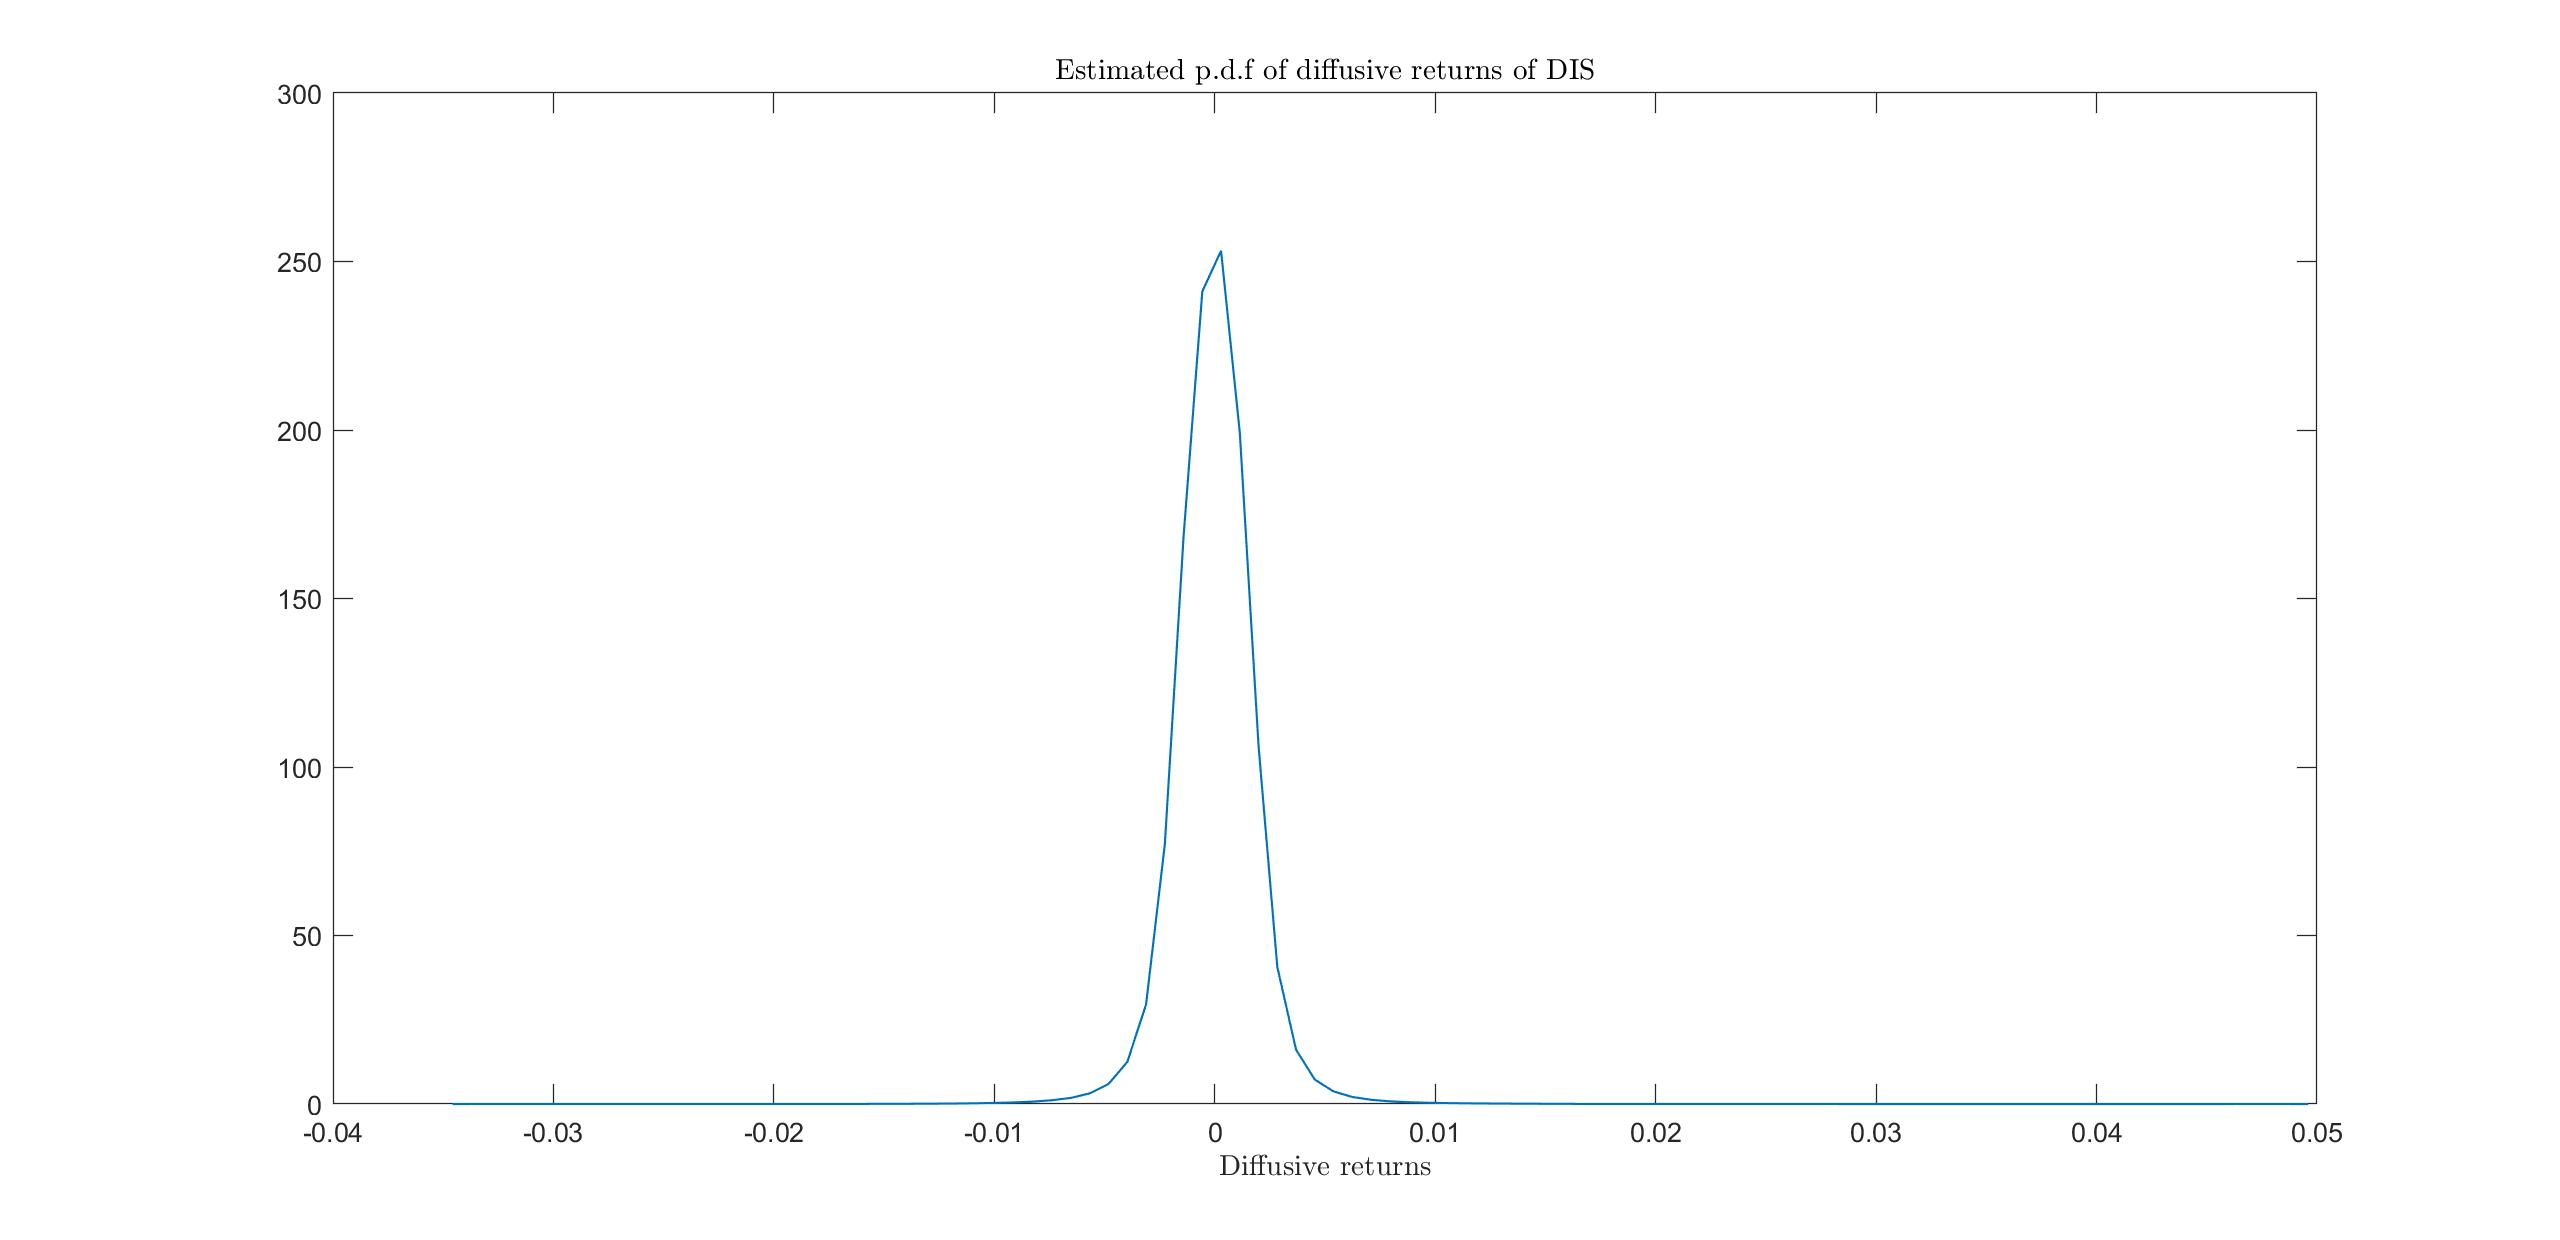
\includegraphics[width=3in]{figures/p3_ex1_g_c_DIS.jpg}
            \end{minipage}
            }
             \subfigure{
           \begin{minipage}[l]{1\linewidth}
           \centering
            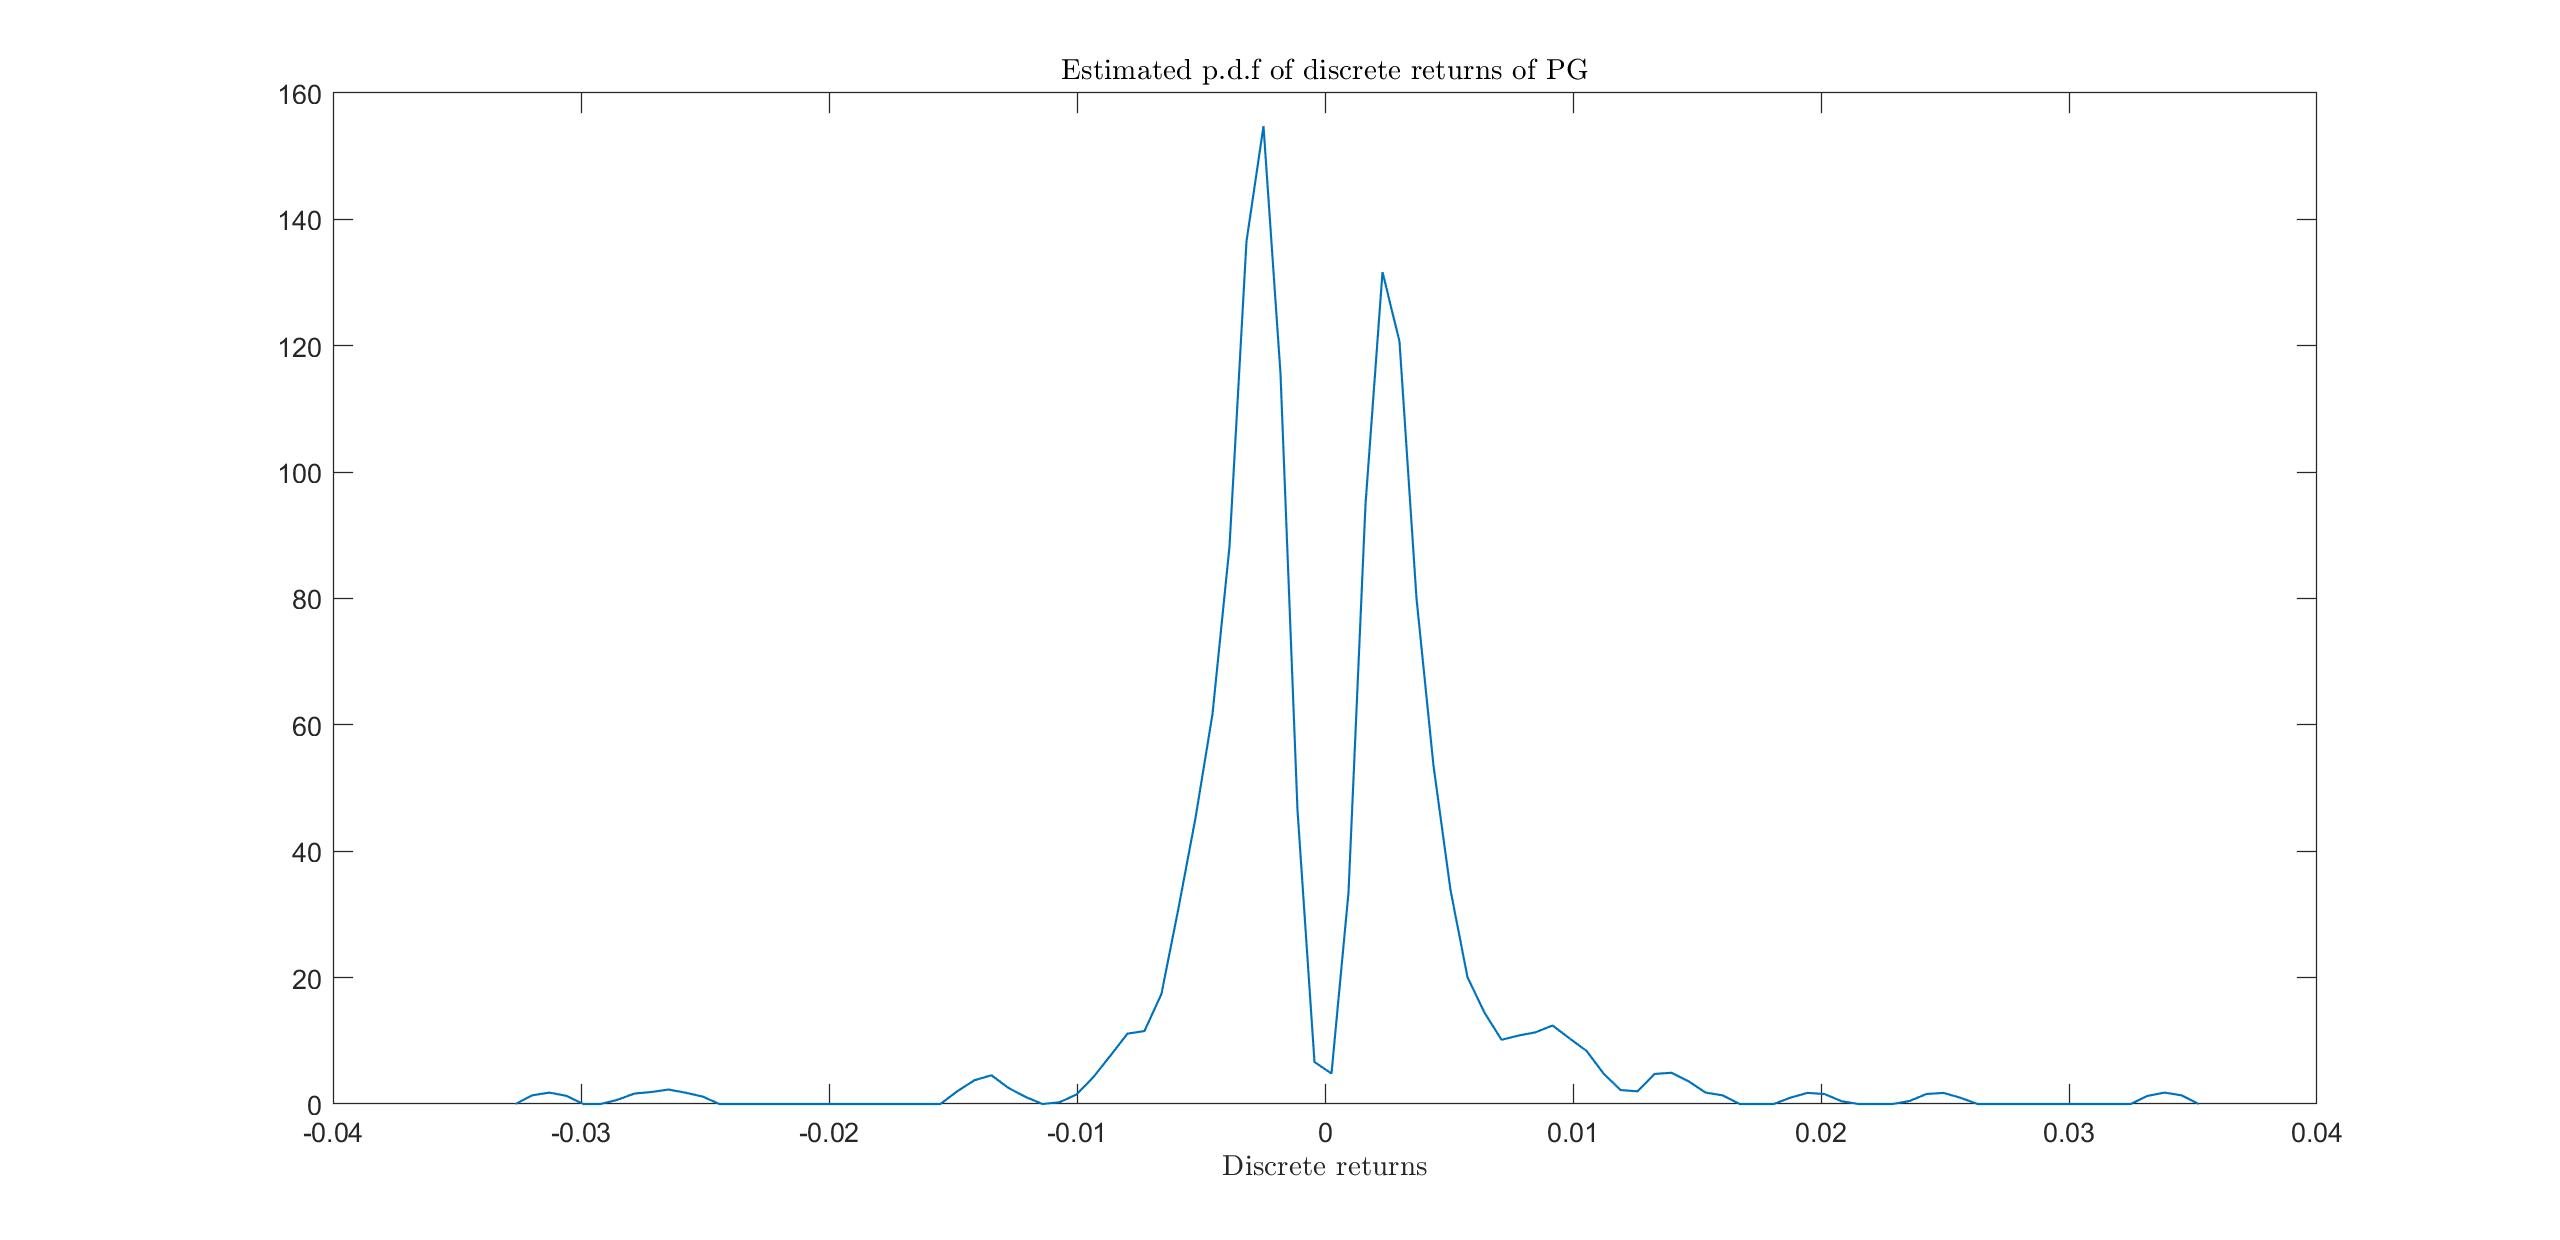
\includegraphics[width=3in]{figures/p3_ex1_g_d.jpg}
            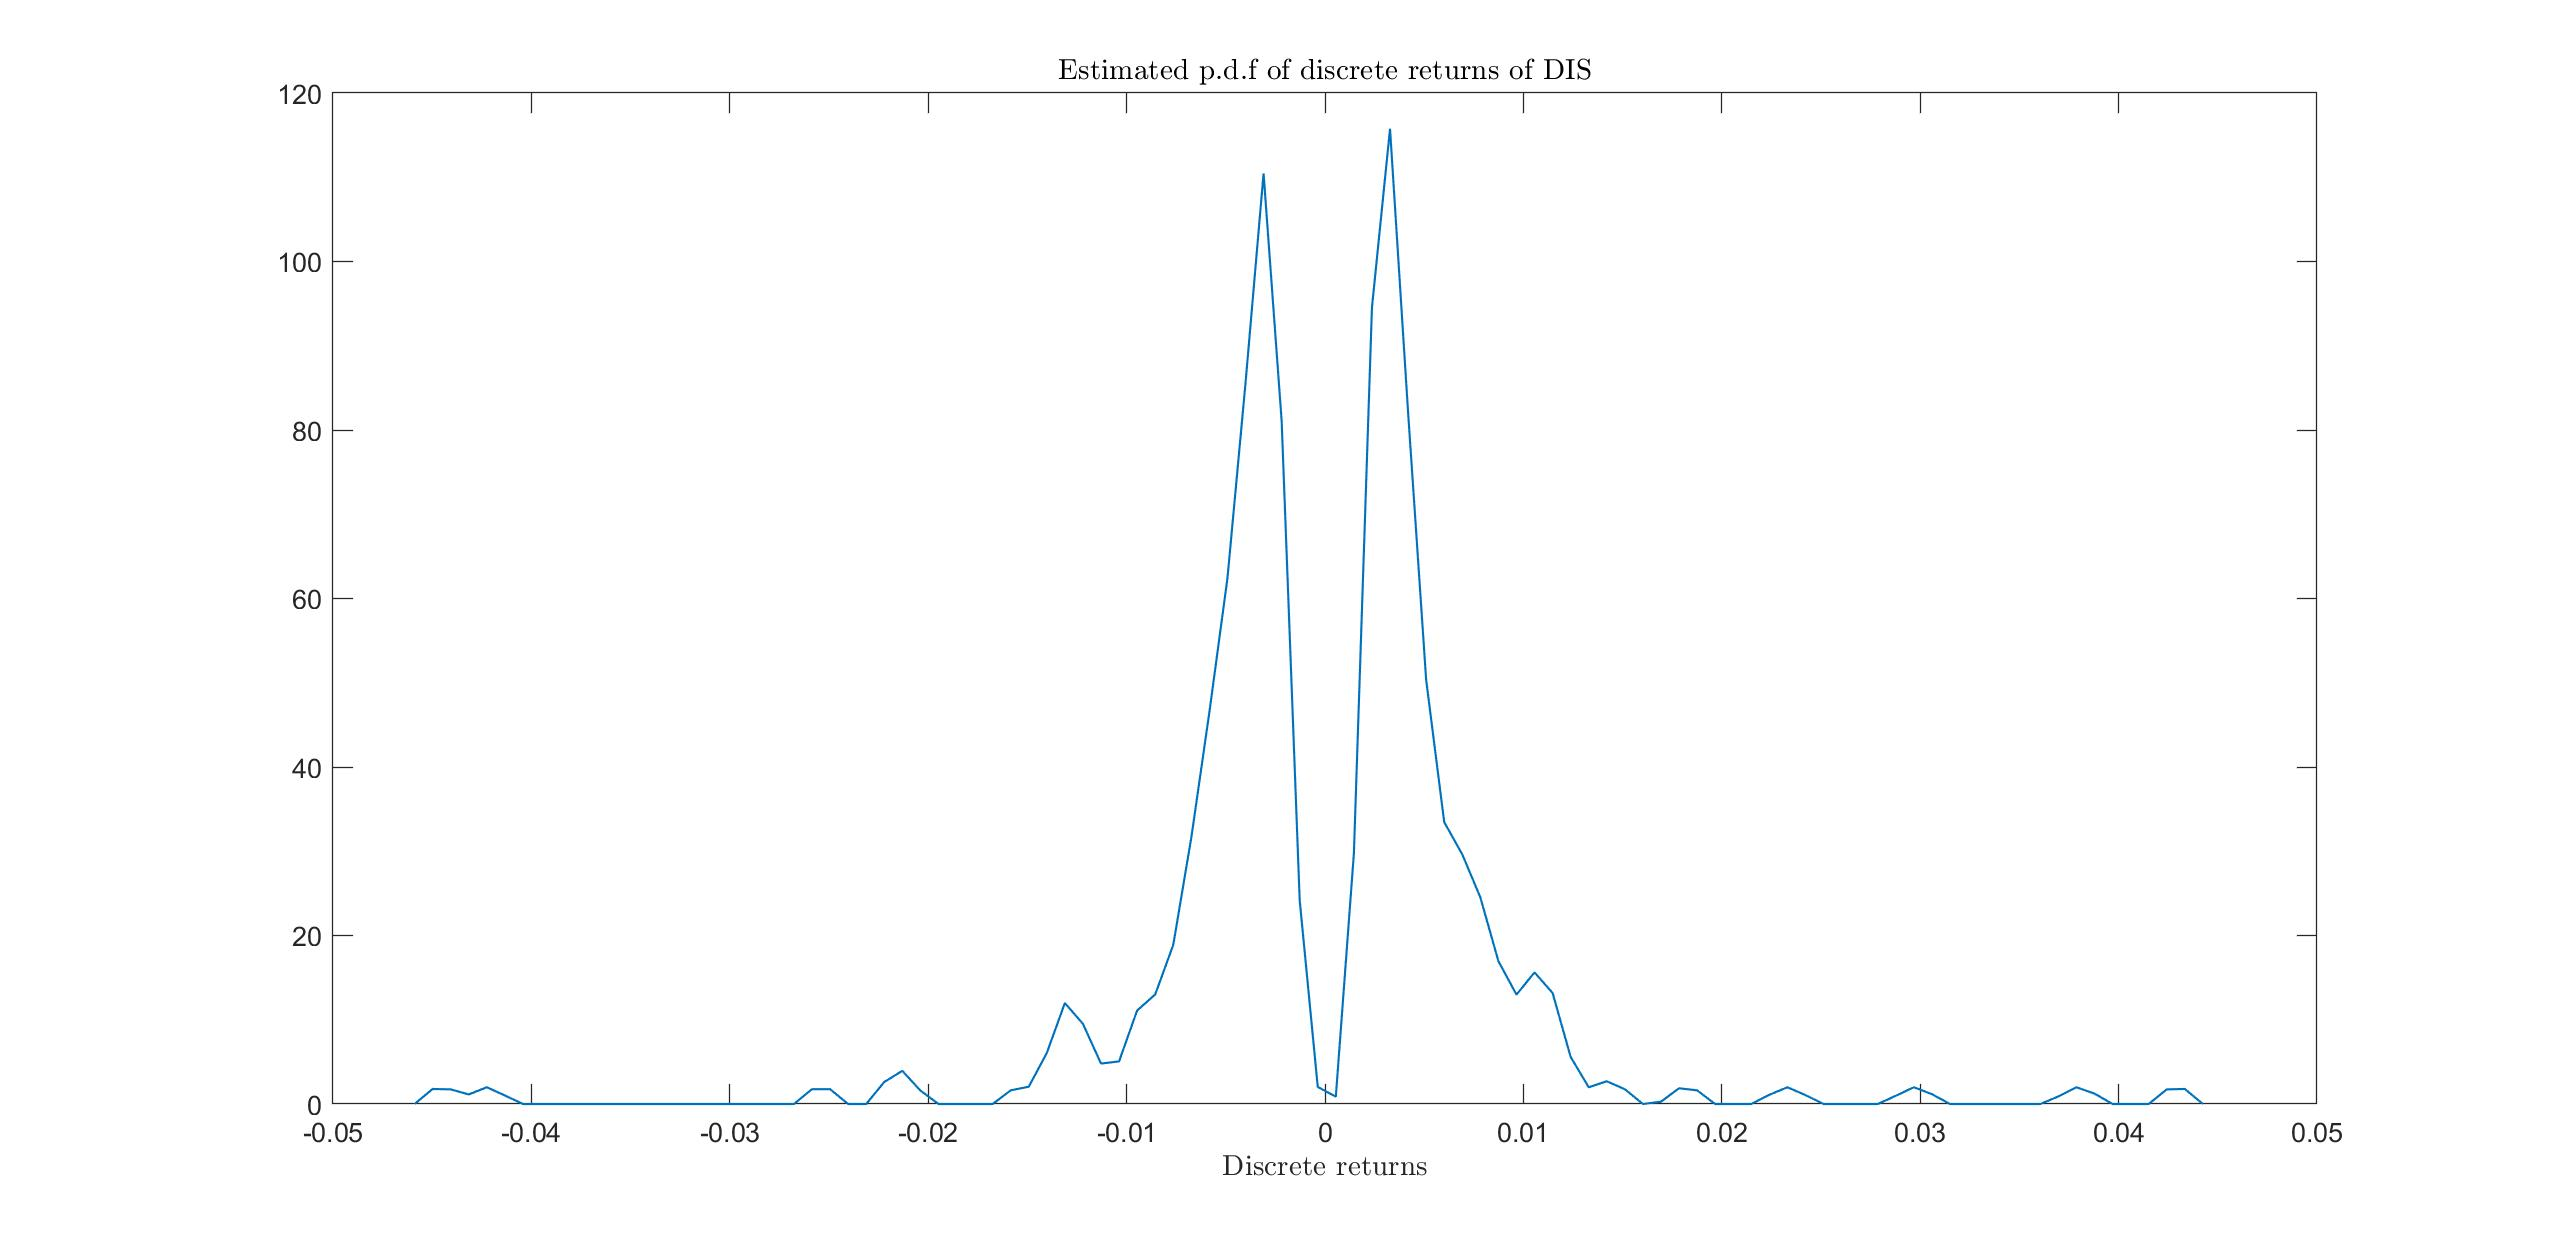
\includegraphics[width=3in]{figures/p3_ex1_g_d_DIS.jpg}
            \end{minipage}
            }
            \centering
            \caption{Estimated p.d.f of diffusive returns and non-zero jump returns for PG and DIS}
\end{figure}
We can see from the figures that, both PG and DIS' diffusive returns' distribution are very similar to normal distribution with mean equals to zero. As for the jump returns, we know that the distributions of jump returns have two peaks. PG's jump returns skews to the left but the skewness isn't very obvious in DIS' jump returns distributions.


\item In the figures of PG's jump returns distribution, it does show that stock crashes are larger and more often than rallies, but this conclusion inverses for the case of DIS. \\

The \textbf{MATLAB} code:
 \lstinputlisting{scripts/p3_ex1_PG.m}

\end{enumerate}
 

\newpage

%---------------------------------------------

\section*{Exercise 2}
  \begin{enumerate}[label=\textbf{(\Alph*)}]
%----A-----
\item
To calculate the truncated variance $TV_t$, we use the diffusive returns we get from Exercise 1 and apply the formula: $TV_t=\sum_{i=1}^{n}(r_{i,t}^c)^2$. 

The follows are the figures.
 \begin{figure}[H]
           \subfigure{
           \begin{minipage}[l]{1\linewidth}
           \centering
             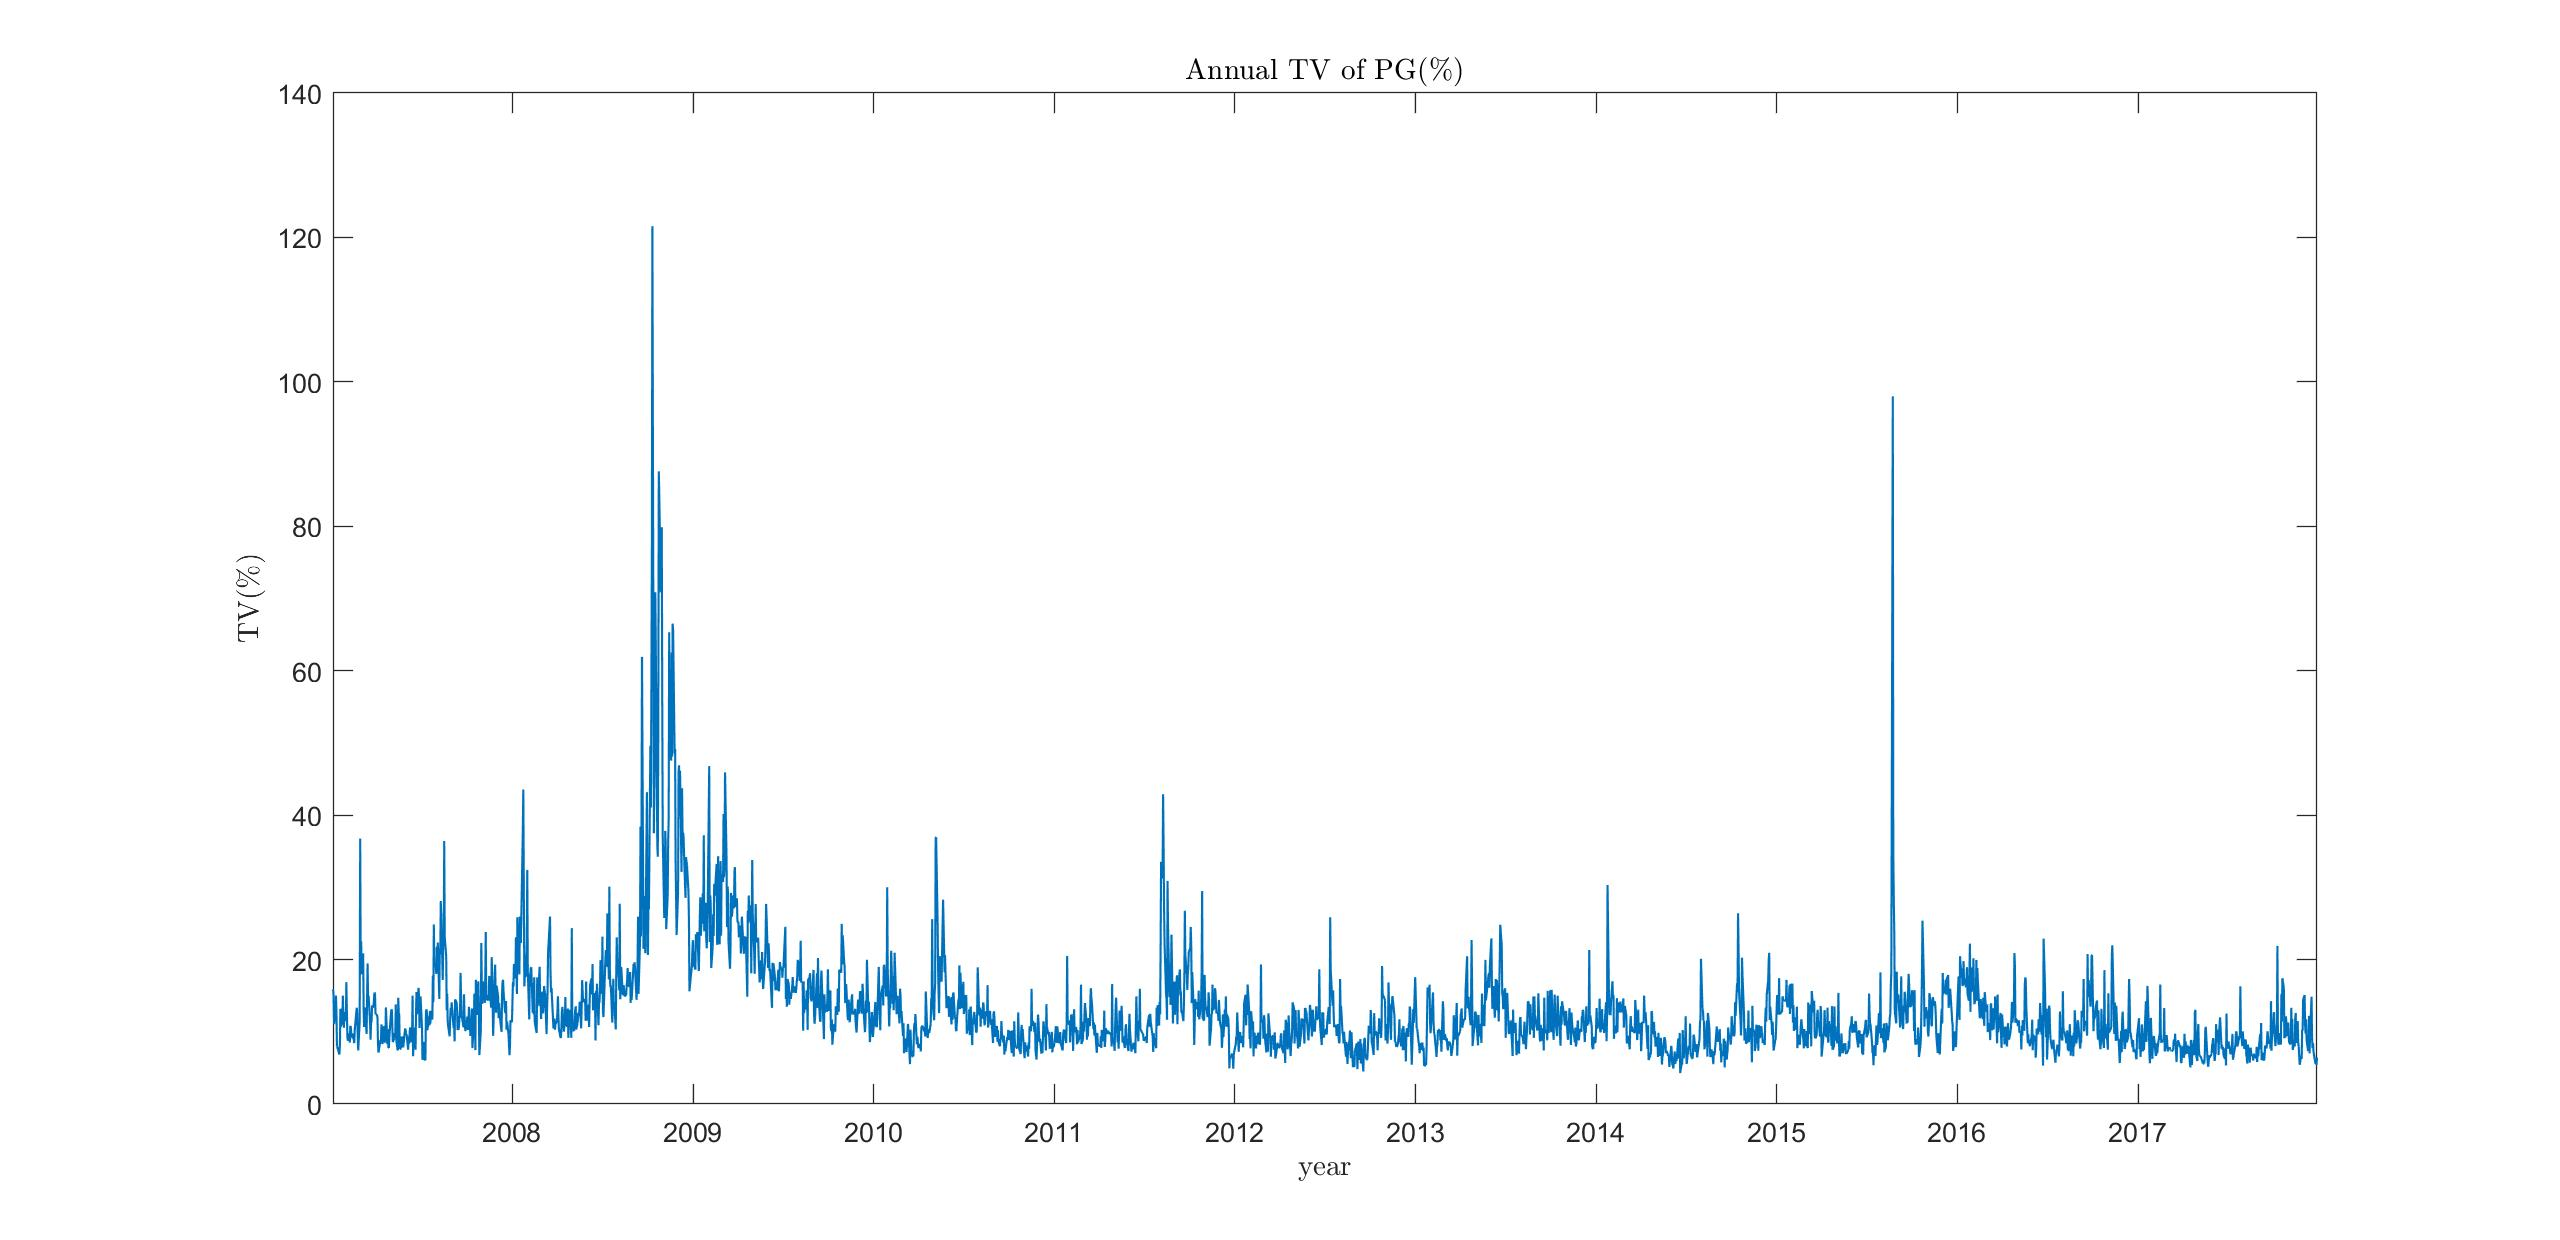
\includegraphics[width=3in]{figures/p3_ex2_a.jpg}
              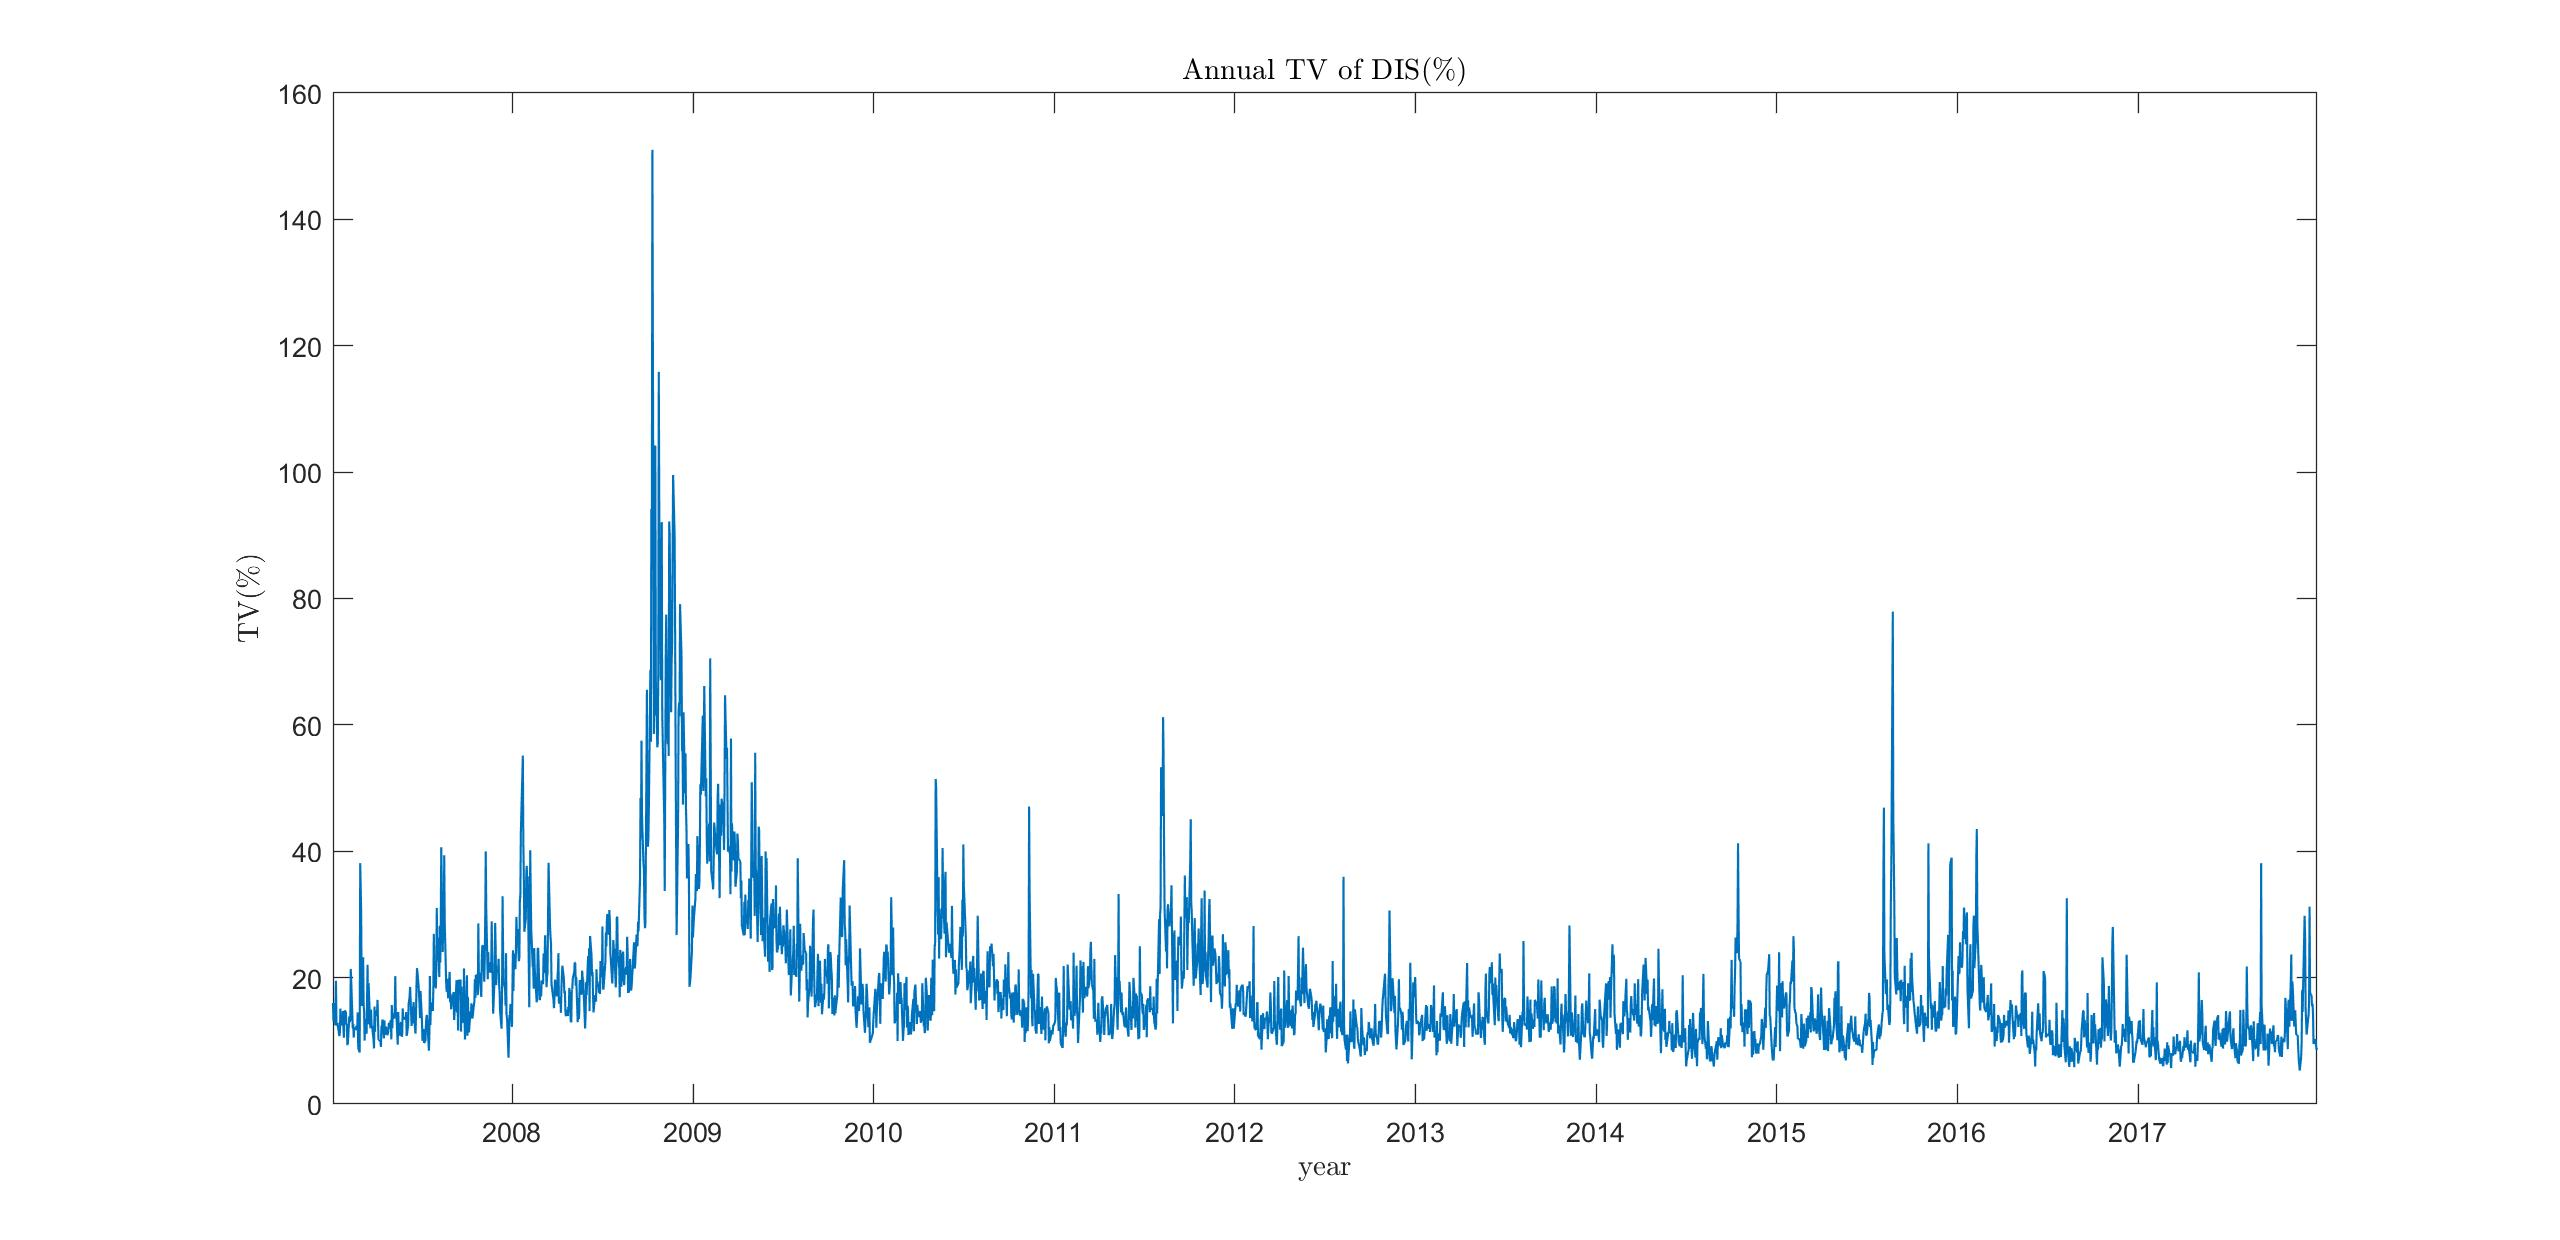
\includegraphics[width=3in]{figures/p3_ex2_a_DIS.jpg}
            \end{minipage}
            }
            \centering
            \caption{Annual TV for PG and DIS}
\end{figure}

From the figures, the range of TV for PG and DIS are (13\%, 120\%) and (18\%,155\%) respectively. We can see that the shape of TV for both stocks are really similar: the value of TV move around 18\% and there are some fluctuations. The TV value is abnormally high at some period, so there may exist some outliers or big price jump in our data for PG and DIS. Besides, we can also observe that DIS' TV is bigger than PG's TV for most of time, which mean that the diffusive returns of DIS have more volatility.\\

The \textbf{MATLAB} code:
   \lstinputlisting{functions/truncated_var_day.m}
   ~~\\
%----B-----
\item
Here are the figures of annual RV and TV for PG and DIS:
 \begin{figure}[H]
           \subfigure{
           \begin{minipage}[l]{1\linewidth}
           \centering
             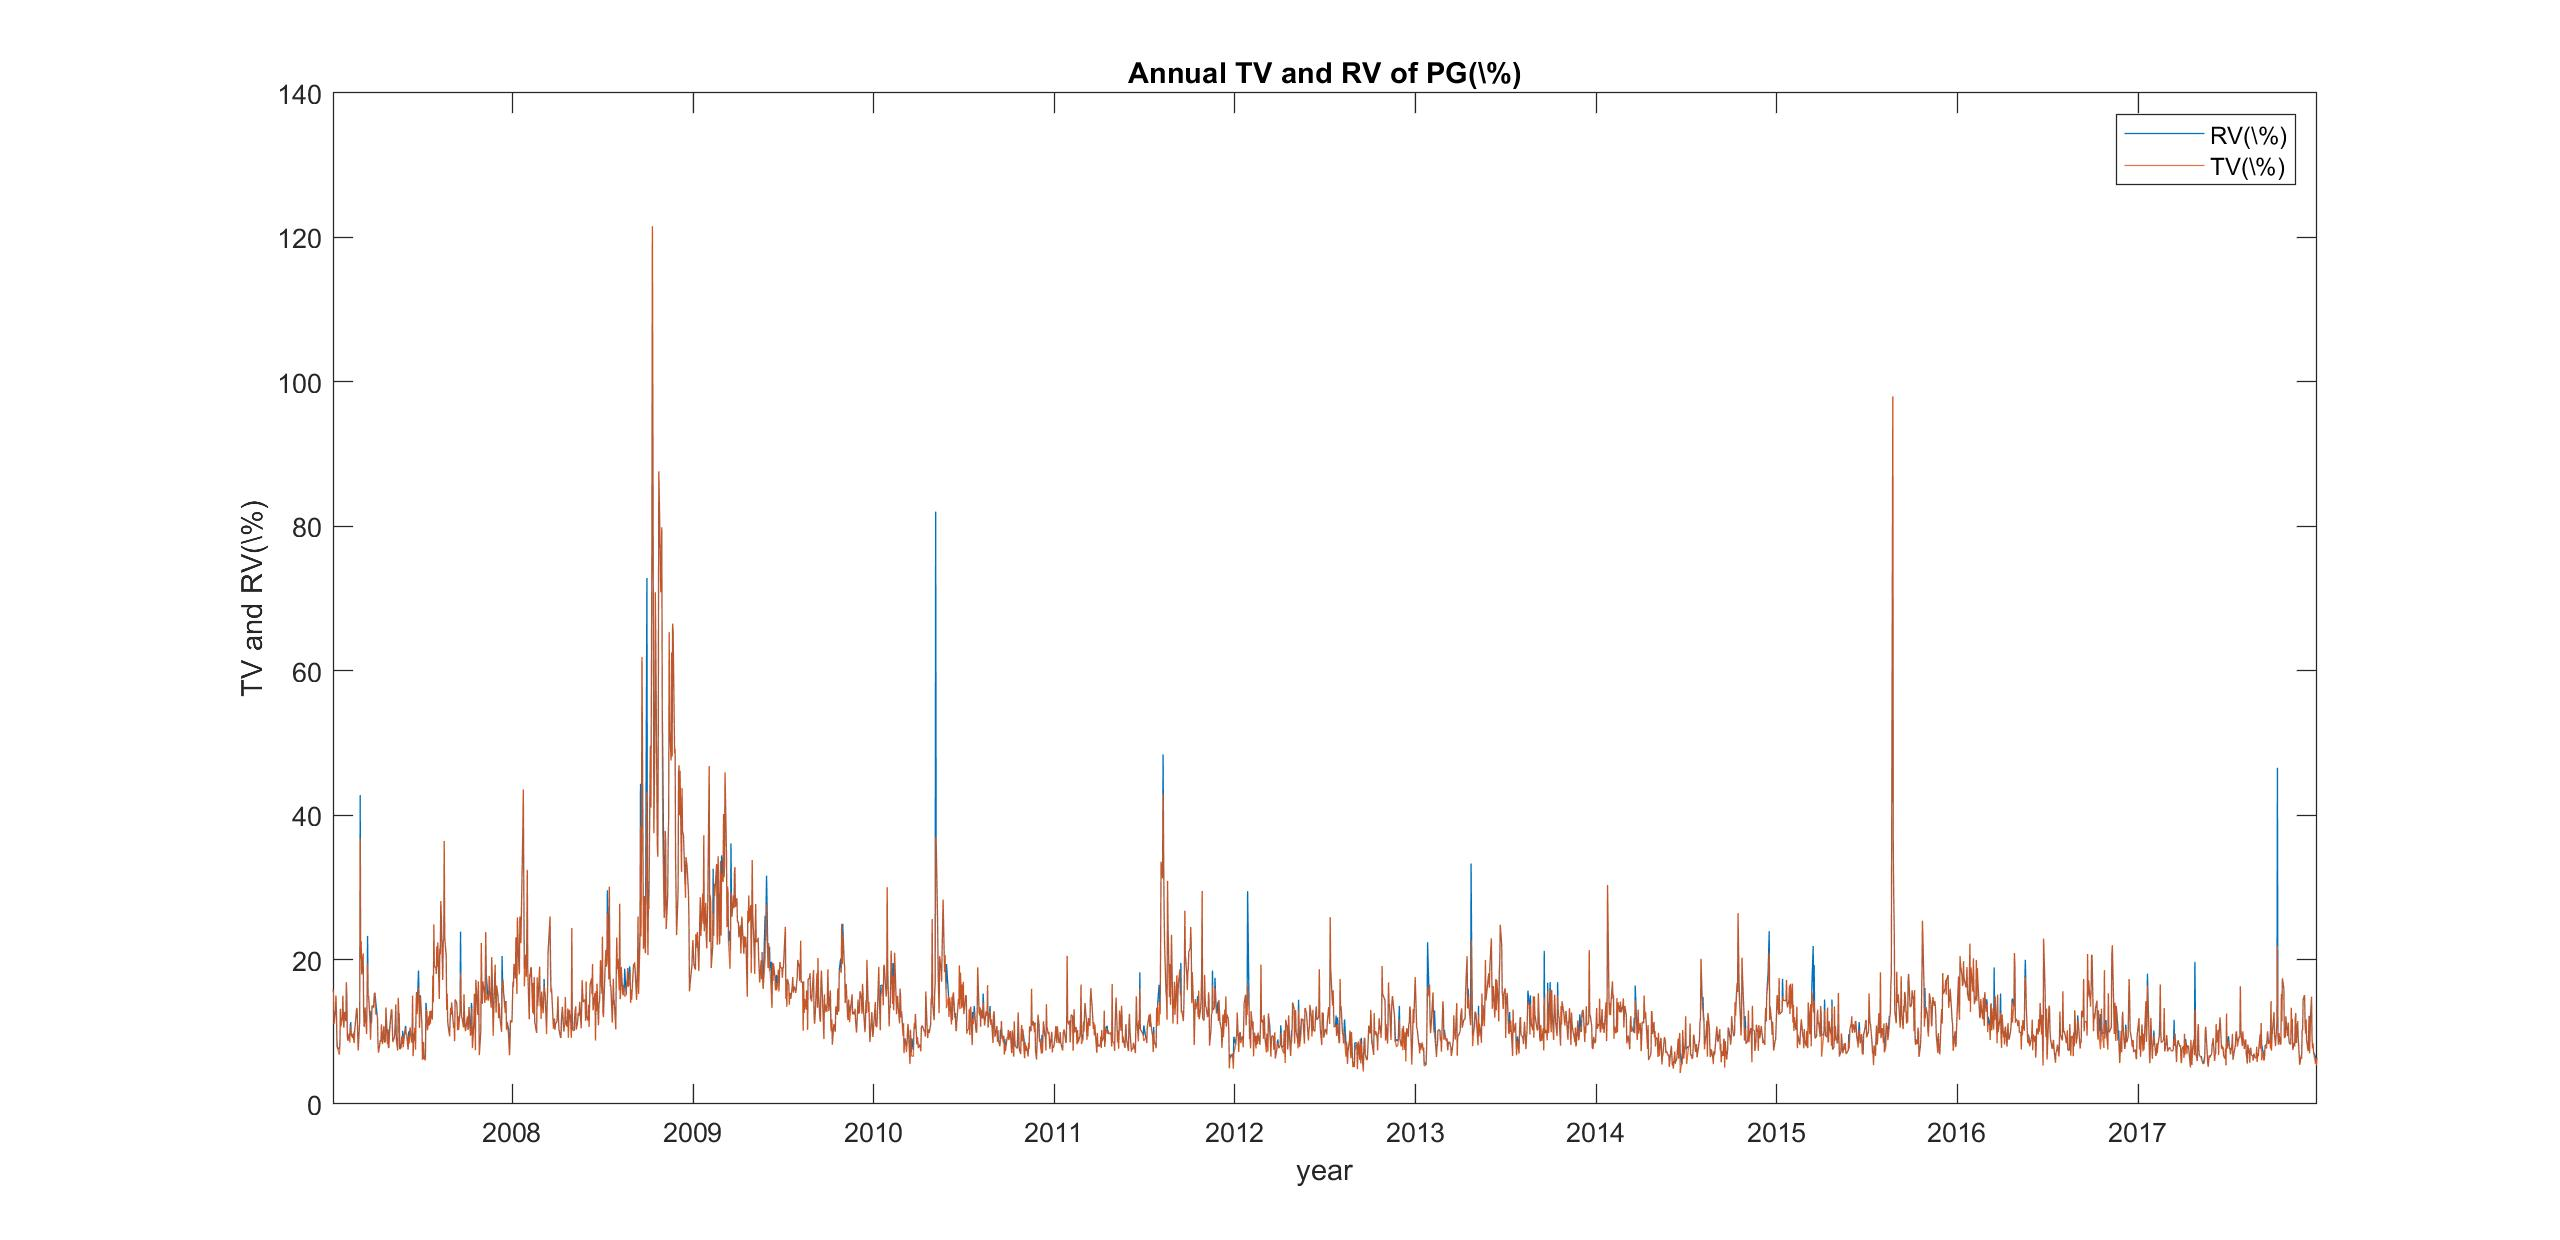
\includegraphics[width=3in]{figures/p3_ex2_b.jpg}
              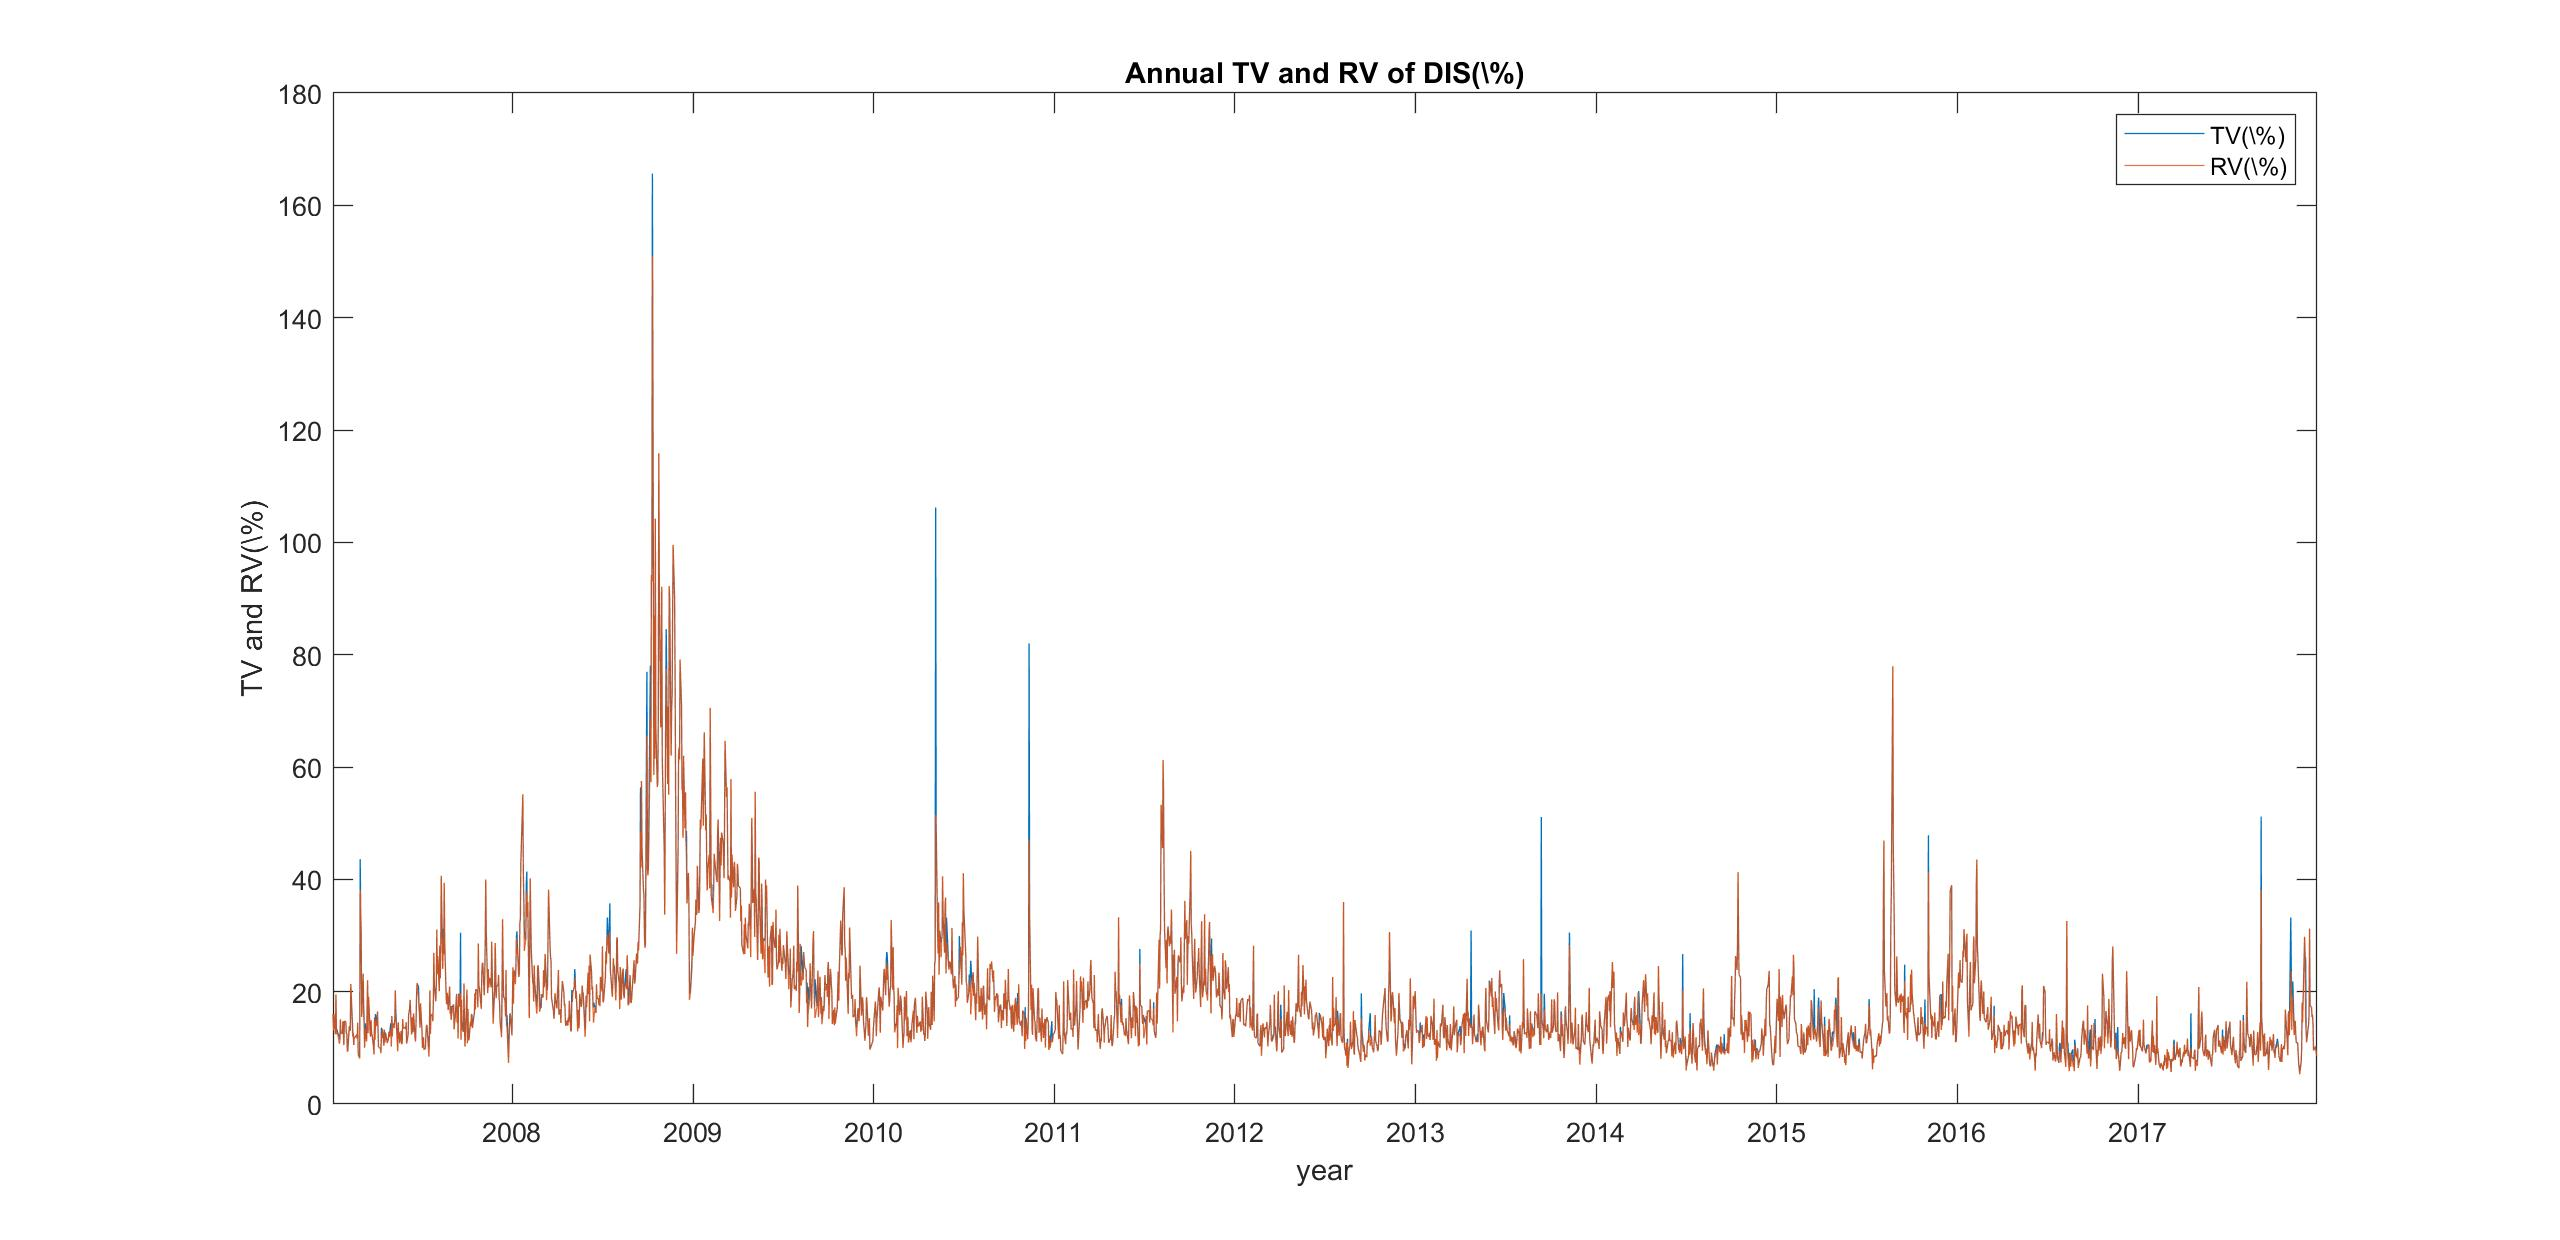
\includegraphics[width=3in]{figures/p3_ex2_b_DIS.jpg}
            \end{minipage}
            }
            \centering
            \caption{Annual RV and TV for PG and DIS}
\end{figure}

From the figures, the range of RV for PG and DIS are (15\%, 120\%) and (18\%,170\%) respectively. We can see that the shape of RV and TV for both stocks are really similar, however, the value of RV is a little larger than TV. These figures show us that by using the diffusive returns instead of the whole regular returns to estimate the volatility of stock's log-returns can give us a smooth(smaller) estimator when the prices of stock exist jumps.\\

%----C-----
\item We can estimate the quartic integrated variance(QIV) by applying the formula: $$\hat{QIV_t}=\frac{1}{3 \Delta_n}\sum_{i=1}^{n}(r_{t,i}^c)^4$$
In order to see the volatility of QIV clearly, we annualized daily QIV. Here are the figures of PG and DIS' QIV estimator.
 \begin{figure}[H]
           \subfigure{
           \begin{minipage}[l]{1\linewidth}
           \centering
             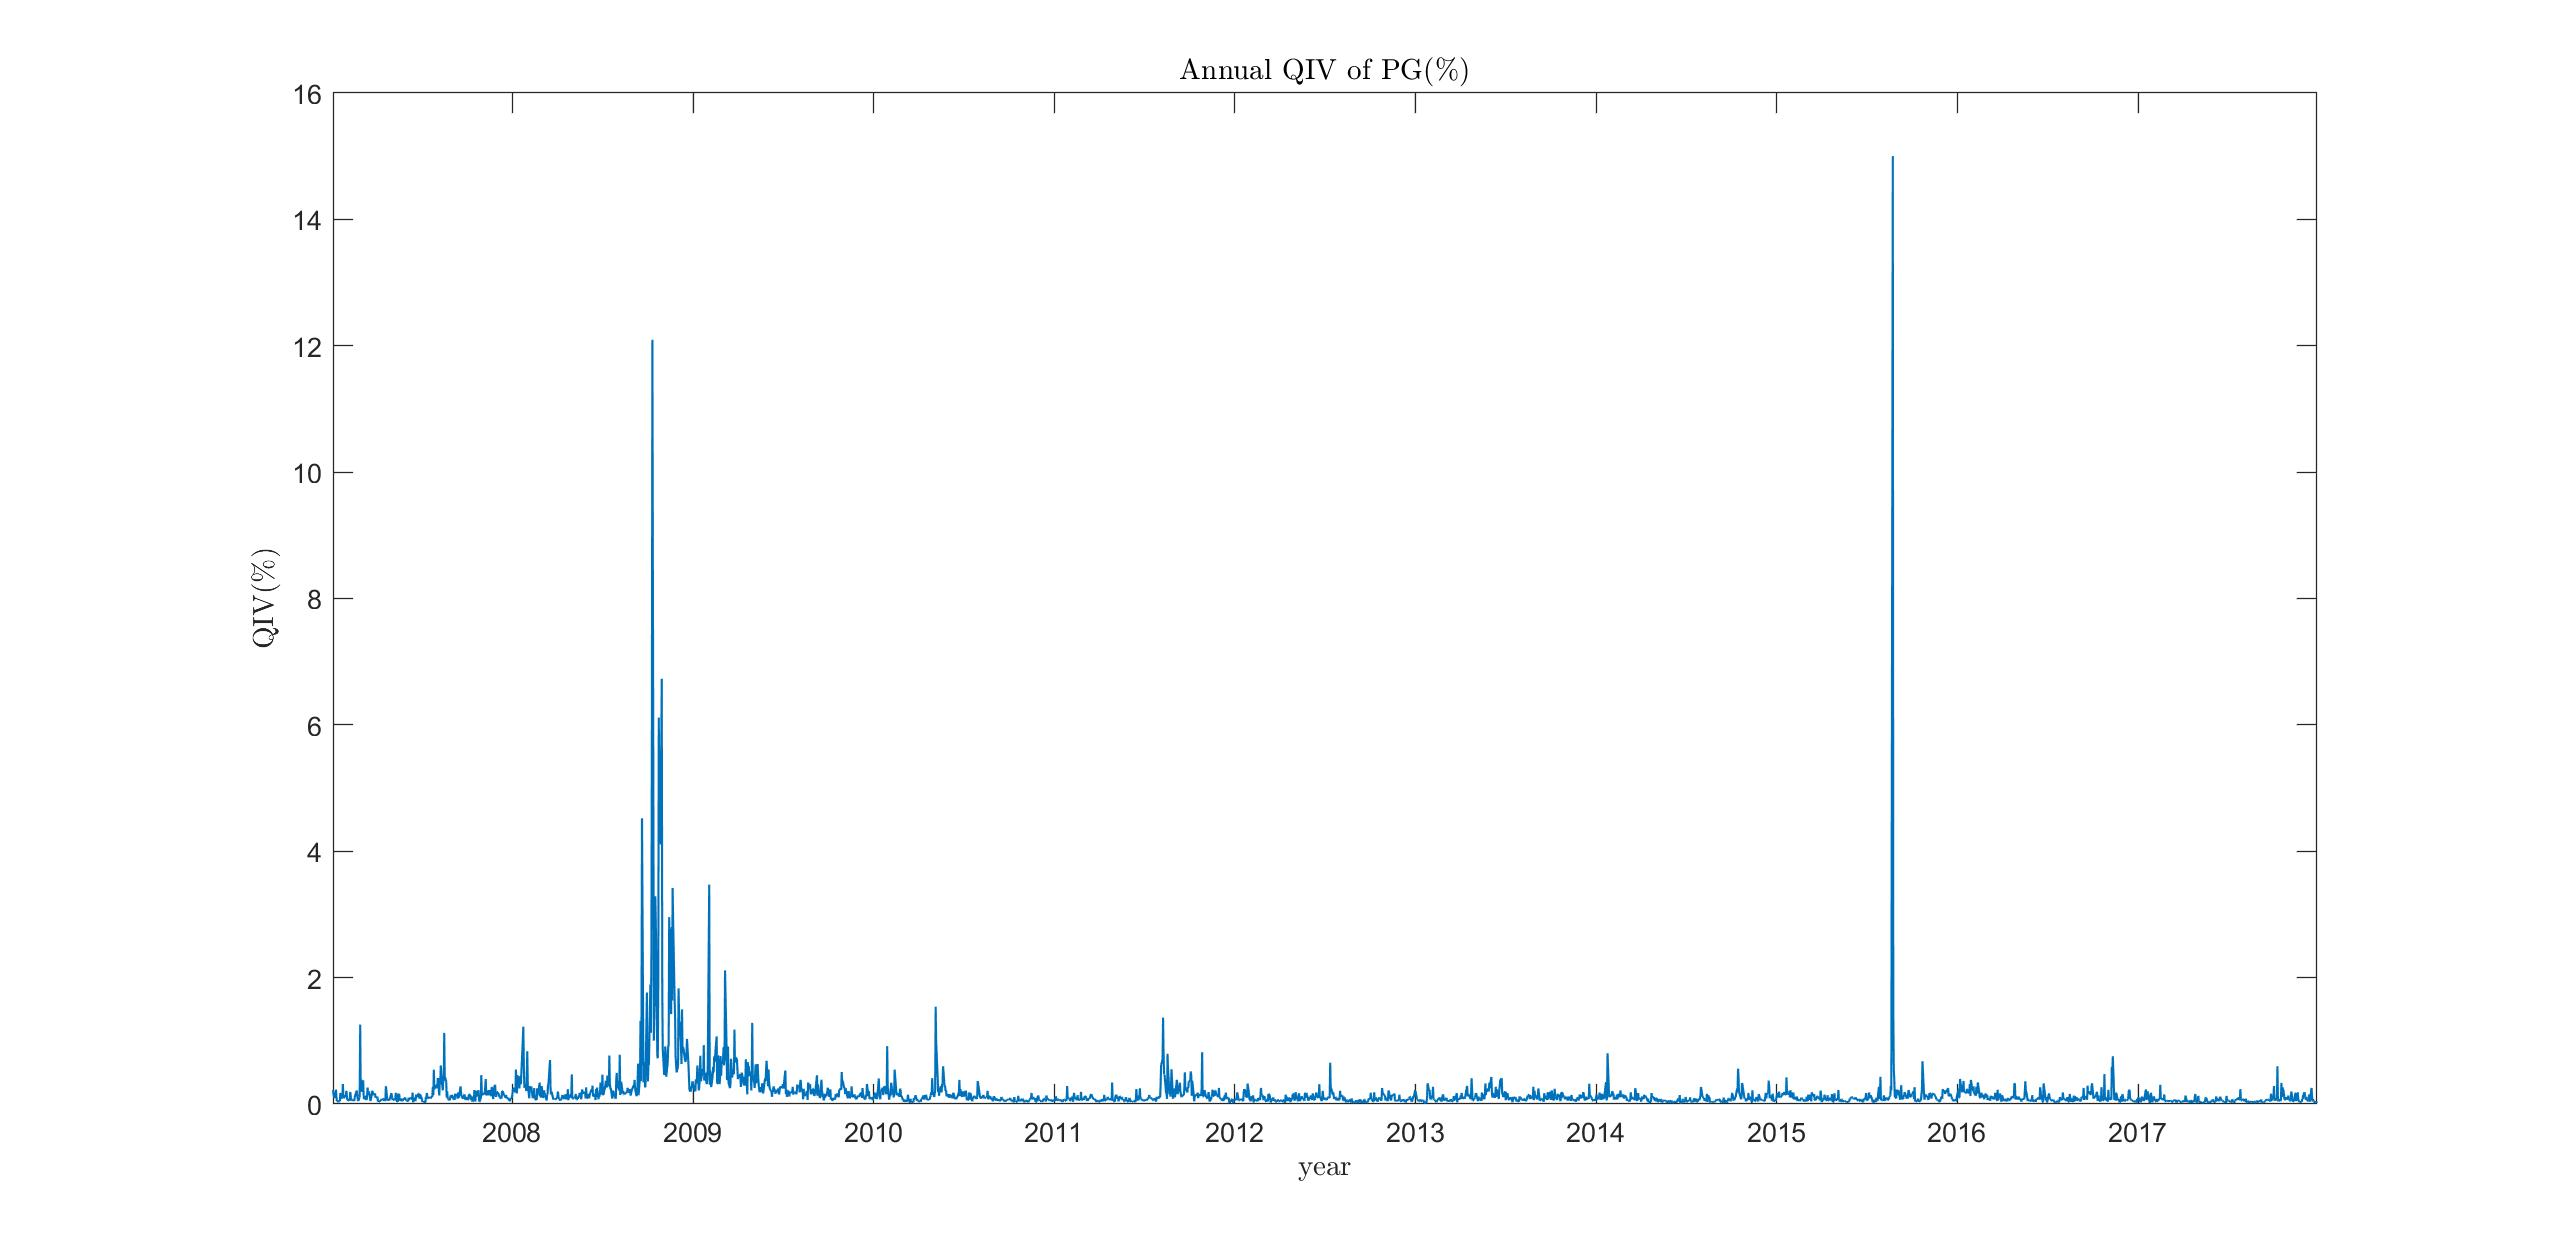
\includegraphics[width=3in]{figures/p3_ex2_c.jpg}
              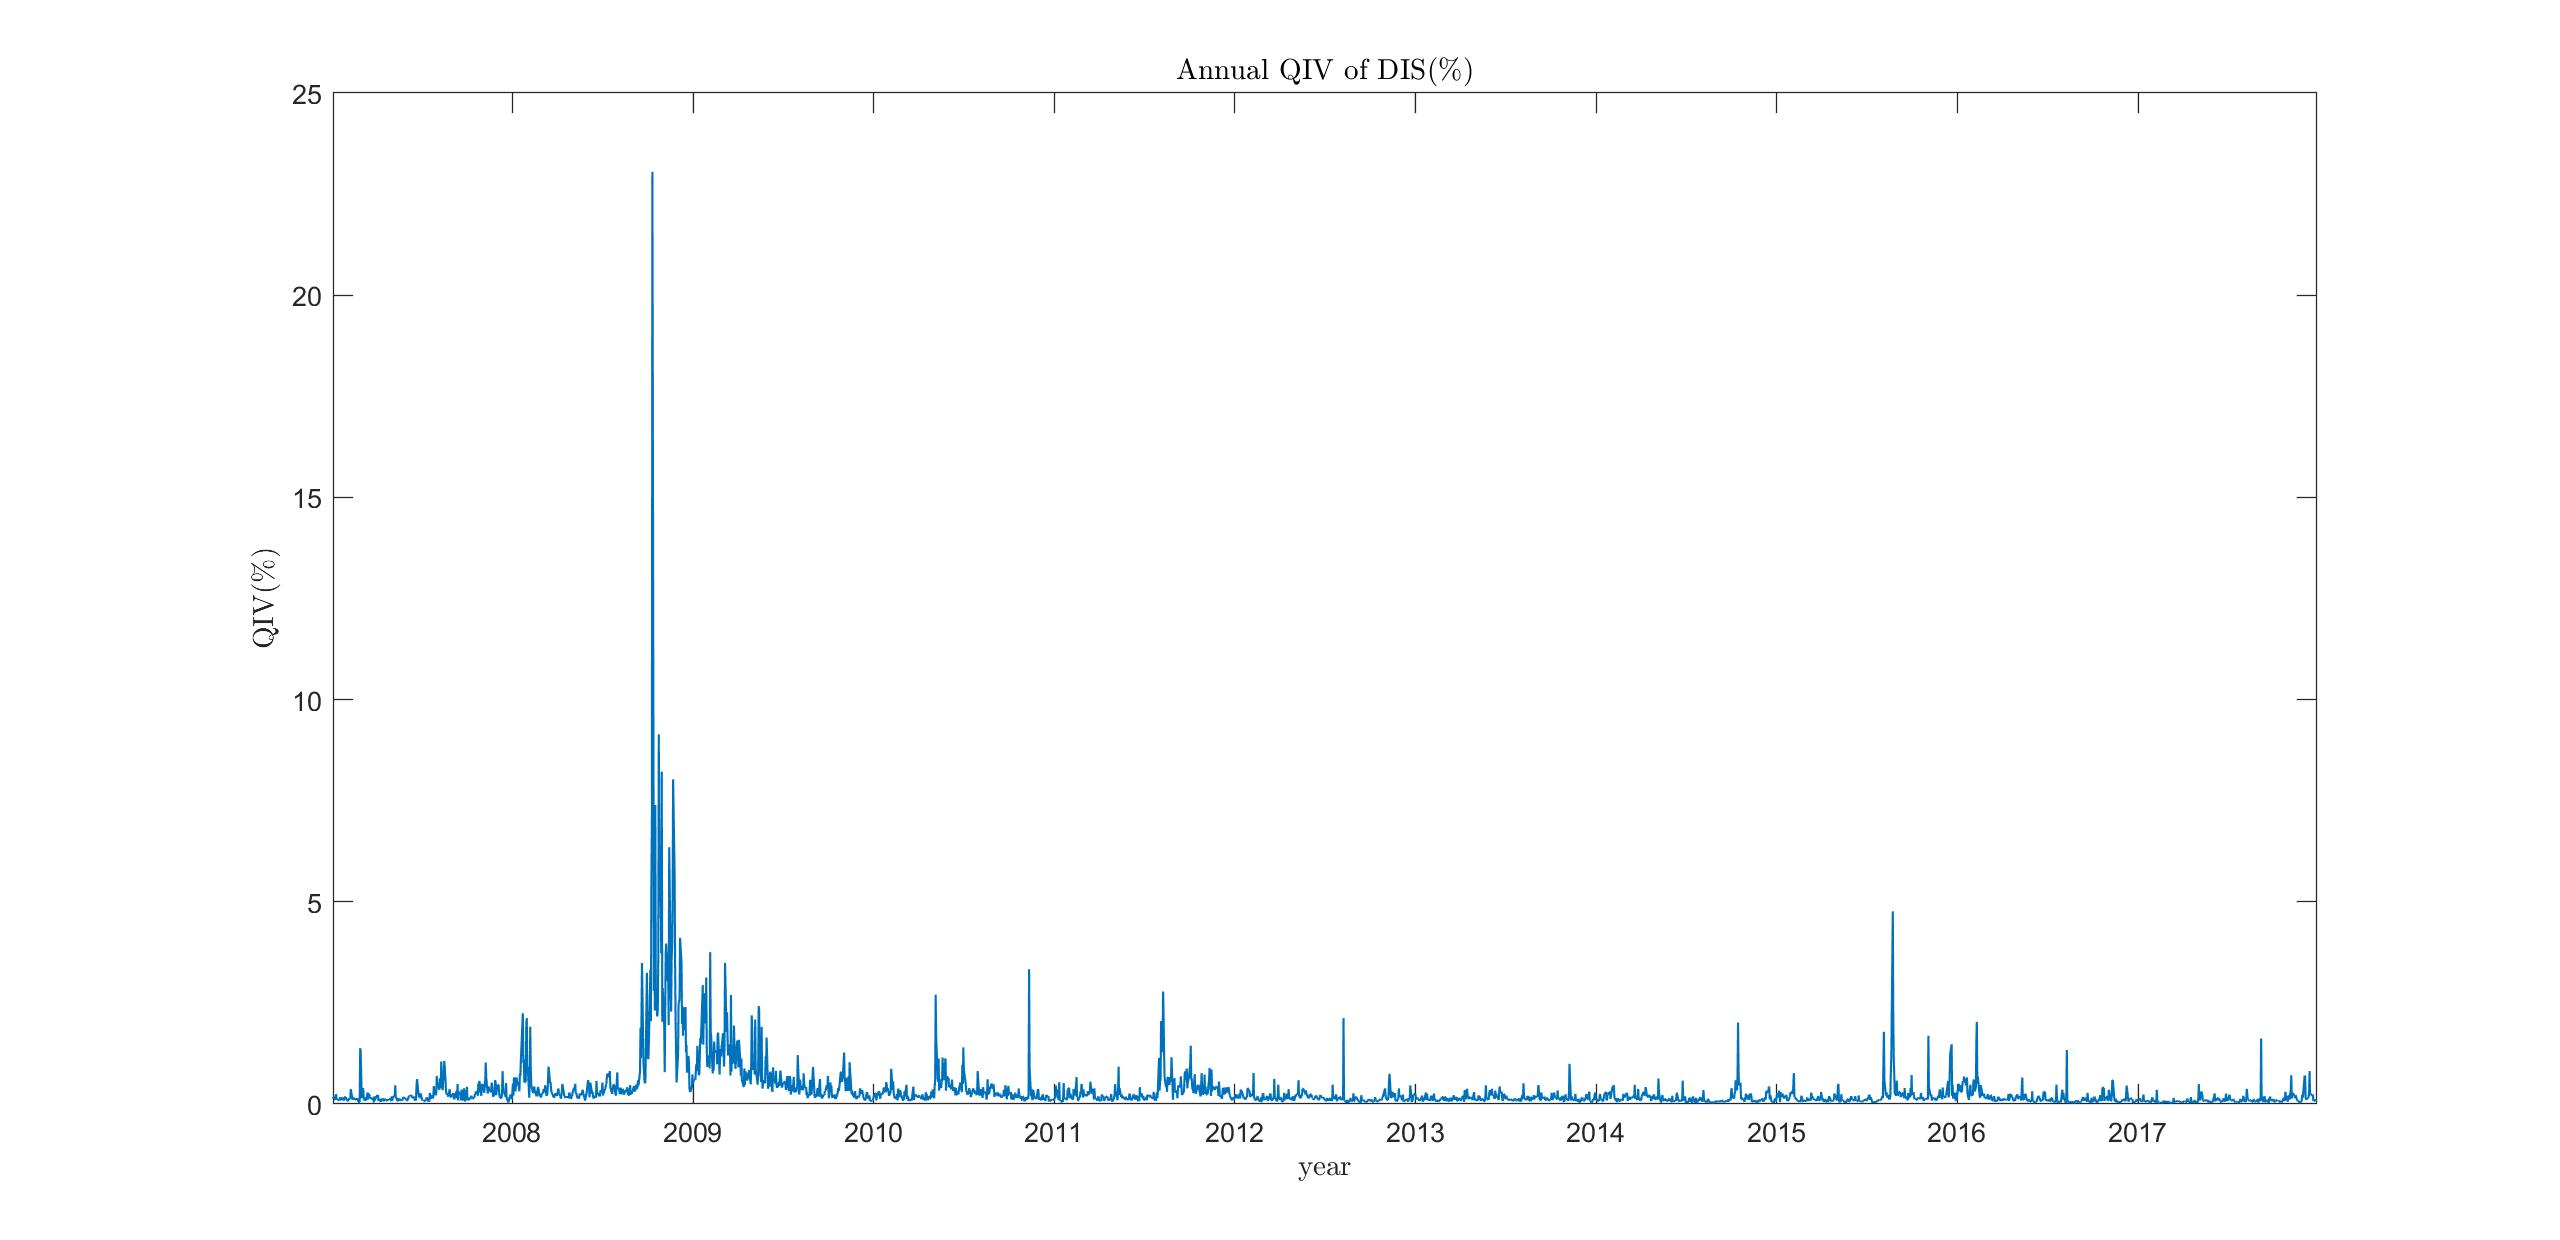
\includegraphics[width=3in]{figures/p3_ex2_c_DIS.jpg}
            \end{minipage}
            }
            \centering
        \caption{Annual estimated QIV for PG and DIS}
\end{figure}

From the figures, we can see that the most value of QIV are very closed to zero. However, we can observe during some period of financial crisis, the QIV can have a large value. For example, around the end of 2008 and the middle of 2015, both PG and DIS' QIV show large volatility and the value of QIV have even reached 12\% and 24\% of end of 2008 and 15\% and 5\% of middle 2015 for PG and DIS respectively. We can say that the QIV of PG and DIS are very sensitive to the whole market situation, which may mean that the correlation between market and PG or DIS may be high. Besides, the figures also verifies that the diffusive returns of DIS have large volatility since the QIV value of DIS is larger. \\
   
The \textbf{MATLAB} code:
   \lstinputlisting{functions/QIV.m}
 
   
%----2D-----
\item
We use this formula to calculate the confidence intervals for IV:$$CI(IV_t,1-\alpha)=[TV_t\pm q_z(\frac{\alpha}{2})\times \sqrt{\frac{2}{3}\sum_{i=1}^{n}(r_{t,i}^c)^4}]$$
where $\alpha$ is the significant level. 

Here are the figures of TV and estimated confidence interval of IV for PG and DIS.

 \begin{figure}[H]
           \subfigure{
           \begin{minipage}[l]{1\linewidth}
           \centering
             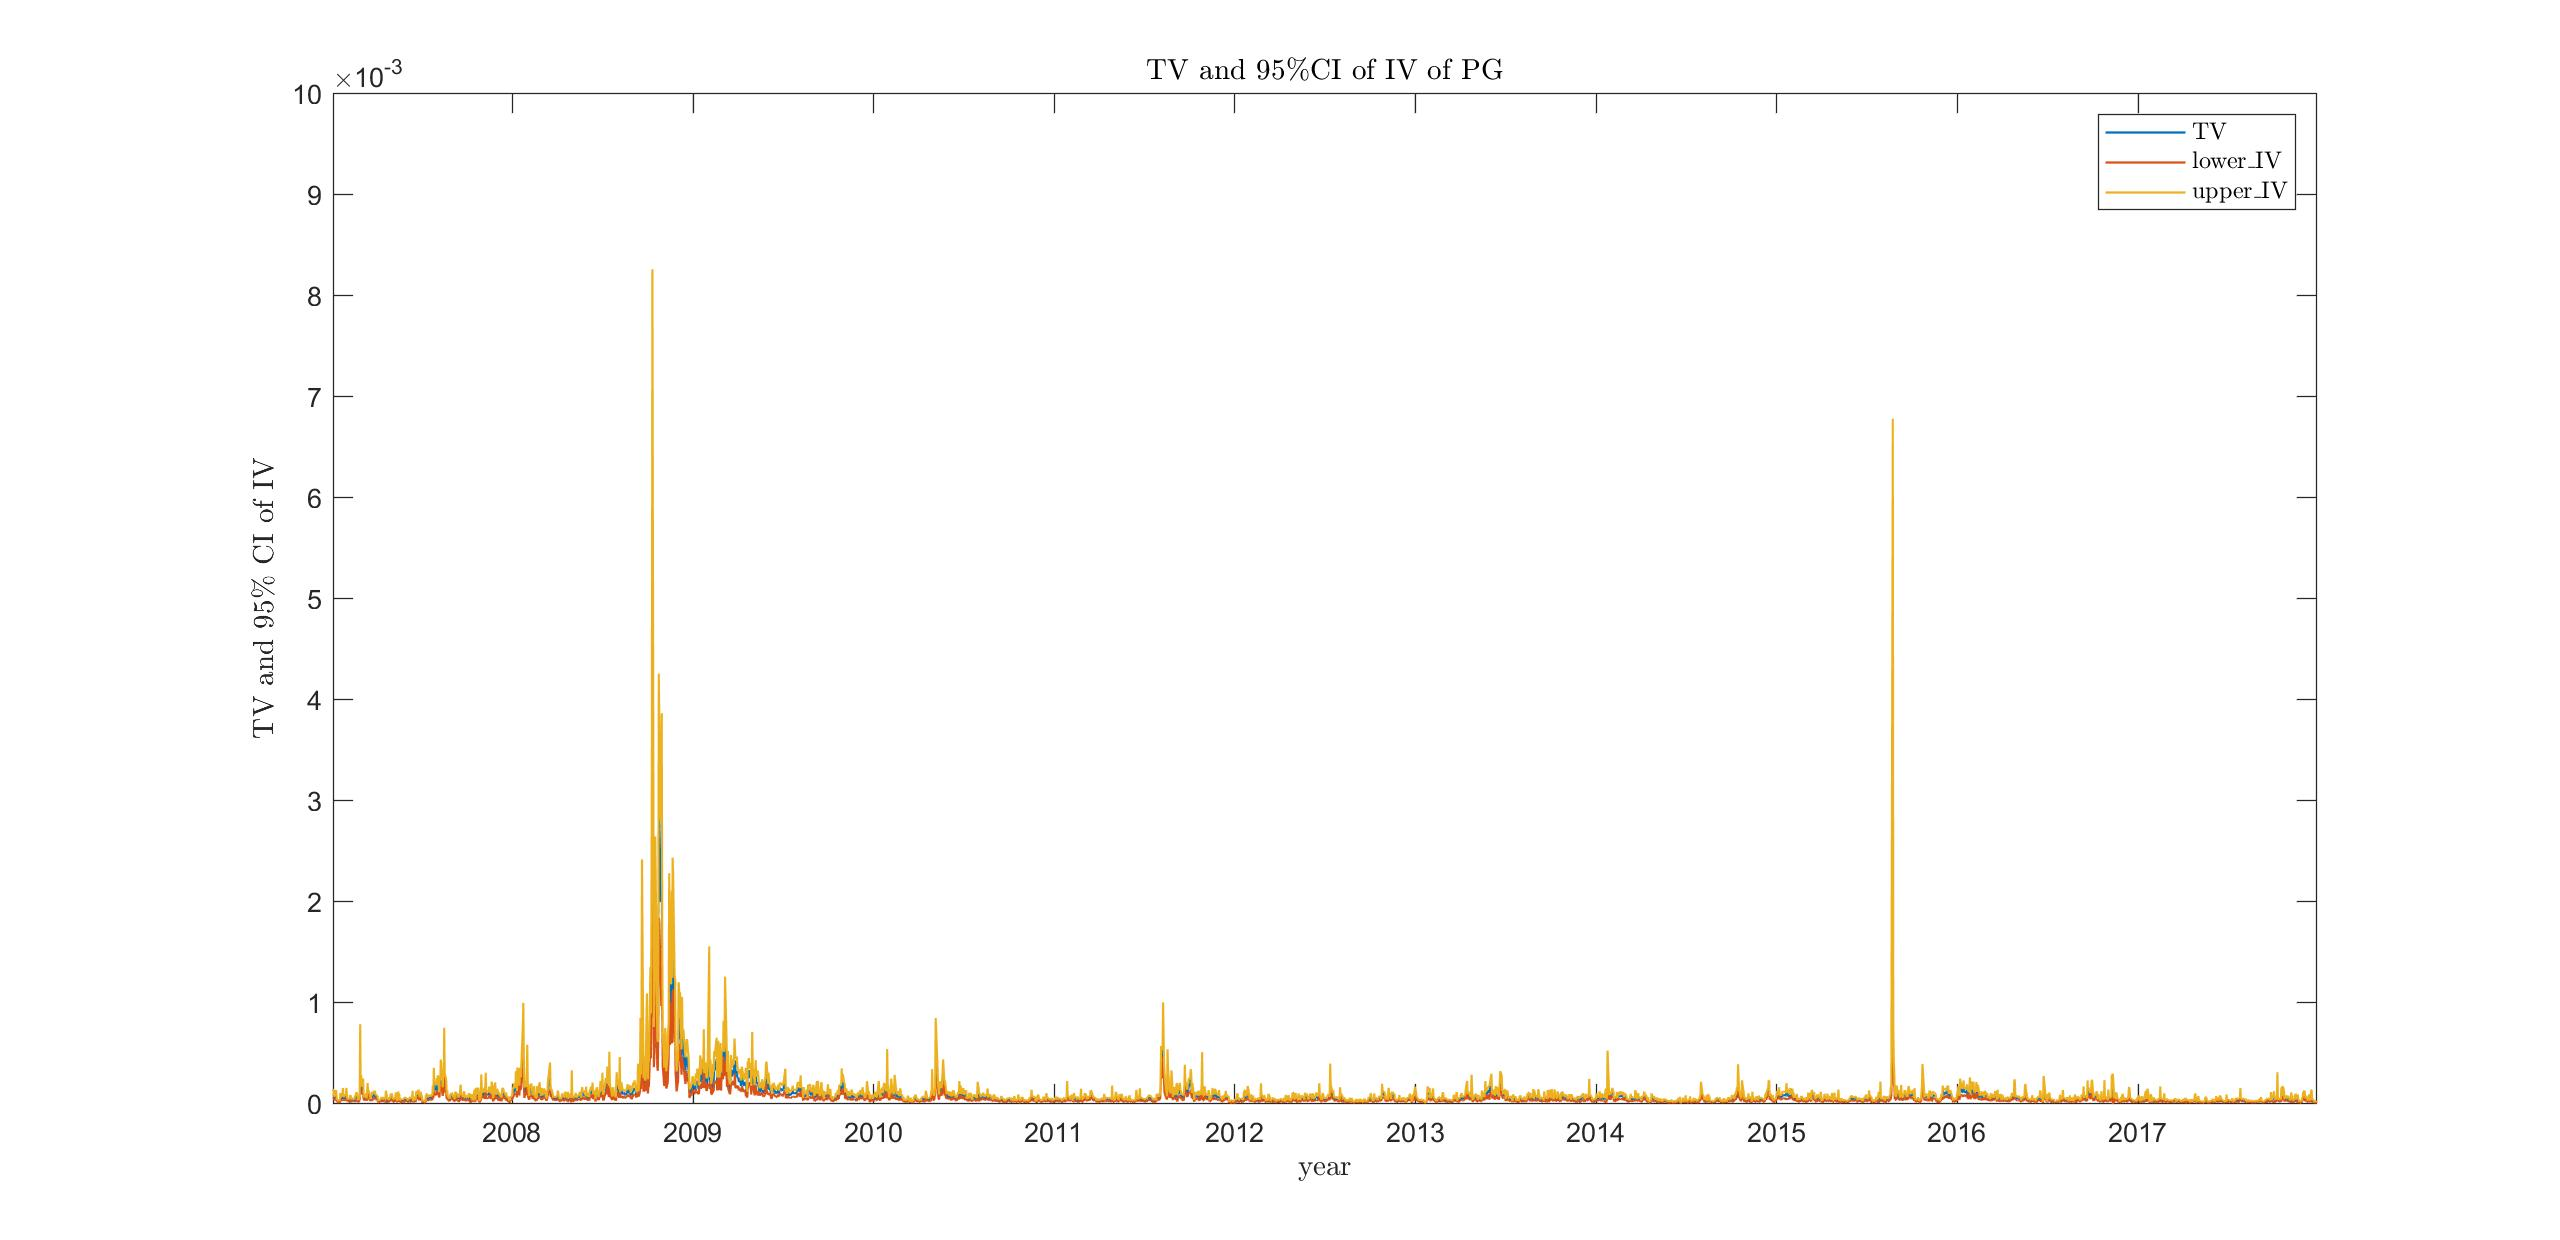
\includegraphics[width=3in]{figures/p3_ex2_d.jpg}
              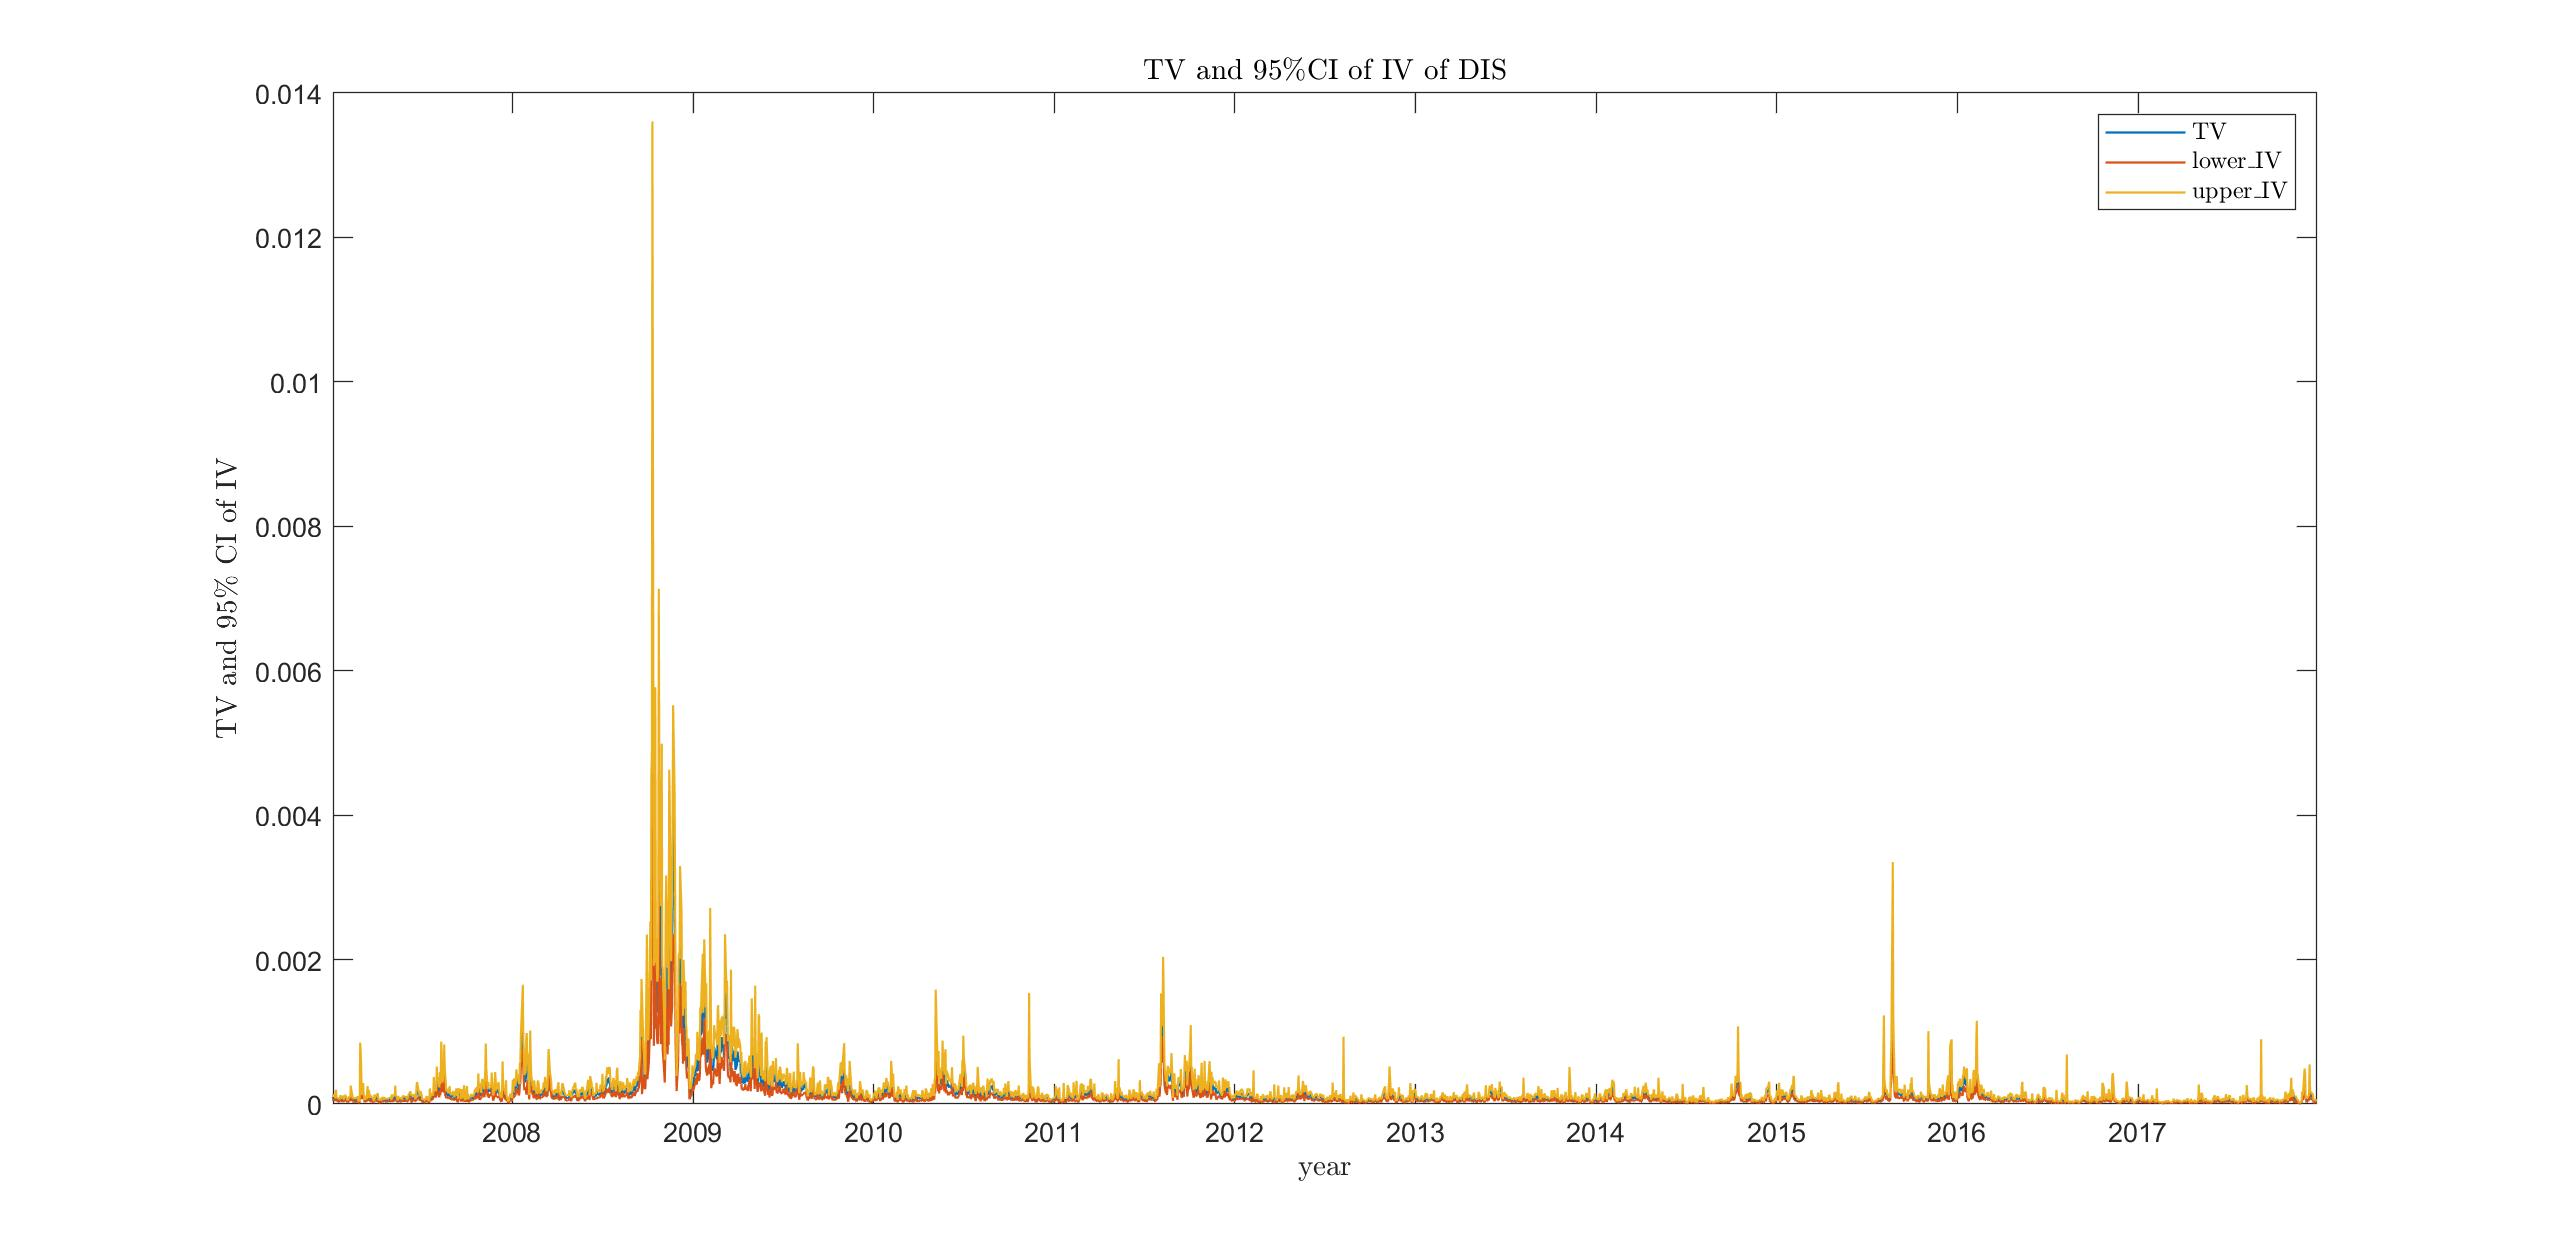
\includegraphics[width=3in]{figures/p3_ex2_d_DIS.jpg}
            \end{minipage}
            }
            \centering
            \caption{TV and Estimated Confidence Interval of IV for PG and DIS}
\end{figure}
%----2E-----
\item 
Now we focus the TV and IV's estimated confidence interval at a specific time interval, say October 2008. Here are the figures.
 \begin{figure}[H]
           \subfigure{
           \begin{minipage}[l]{1\linewidth}
           \centering
             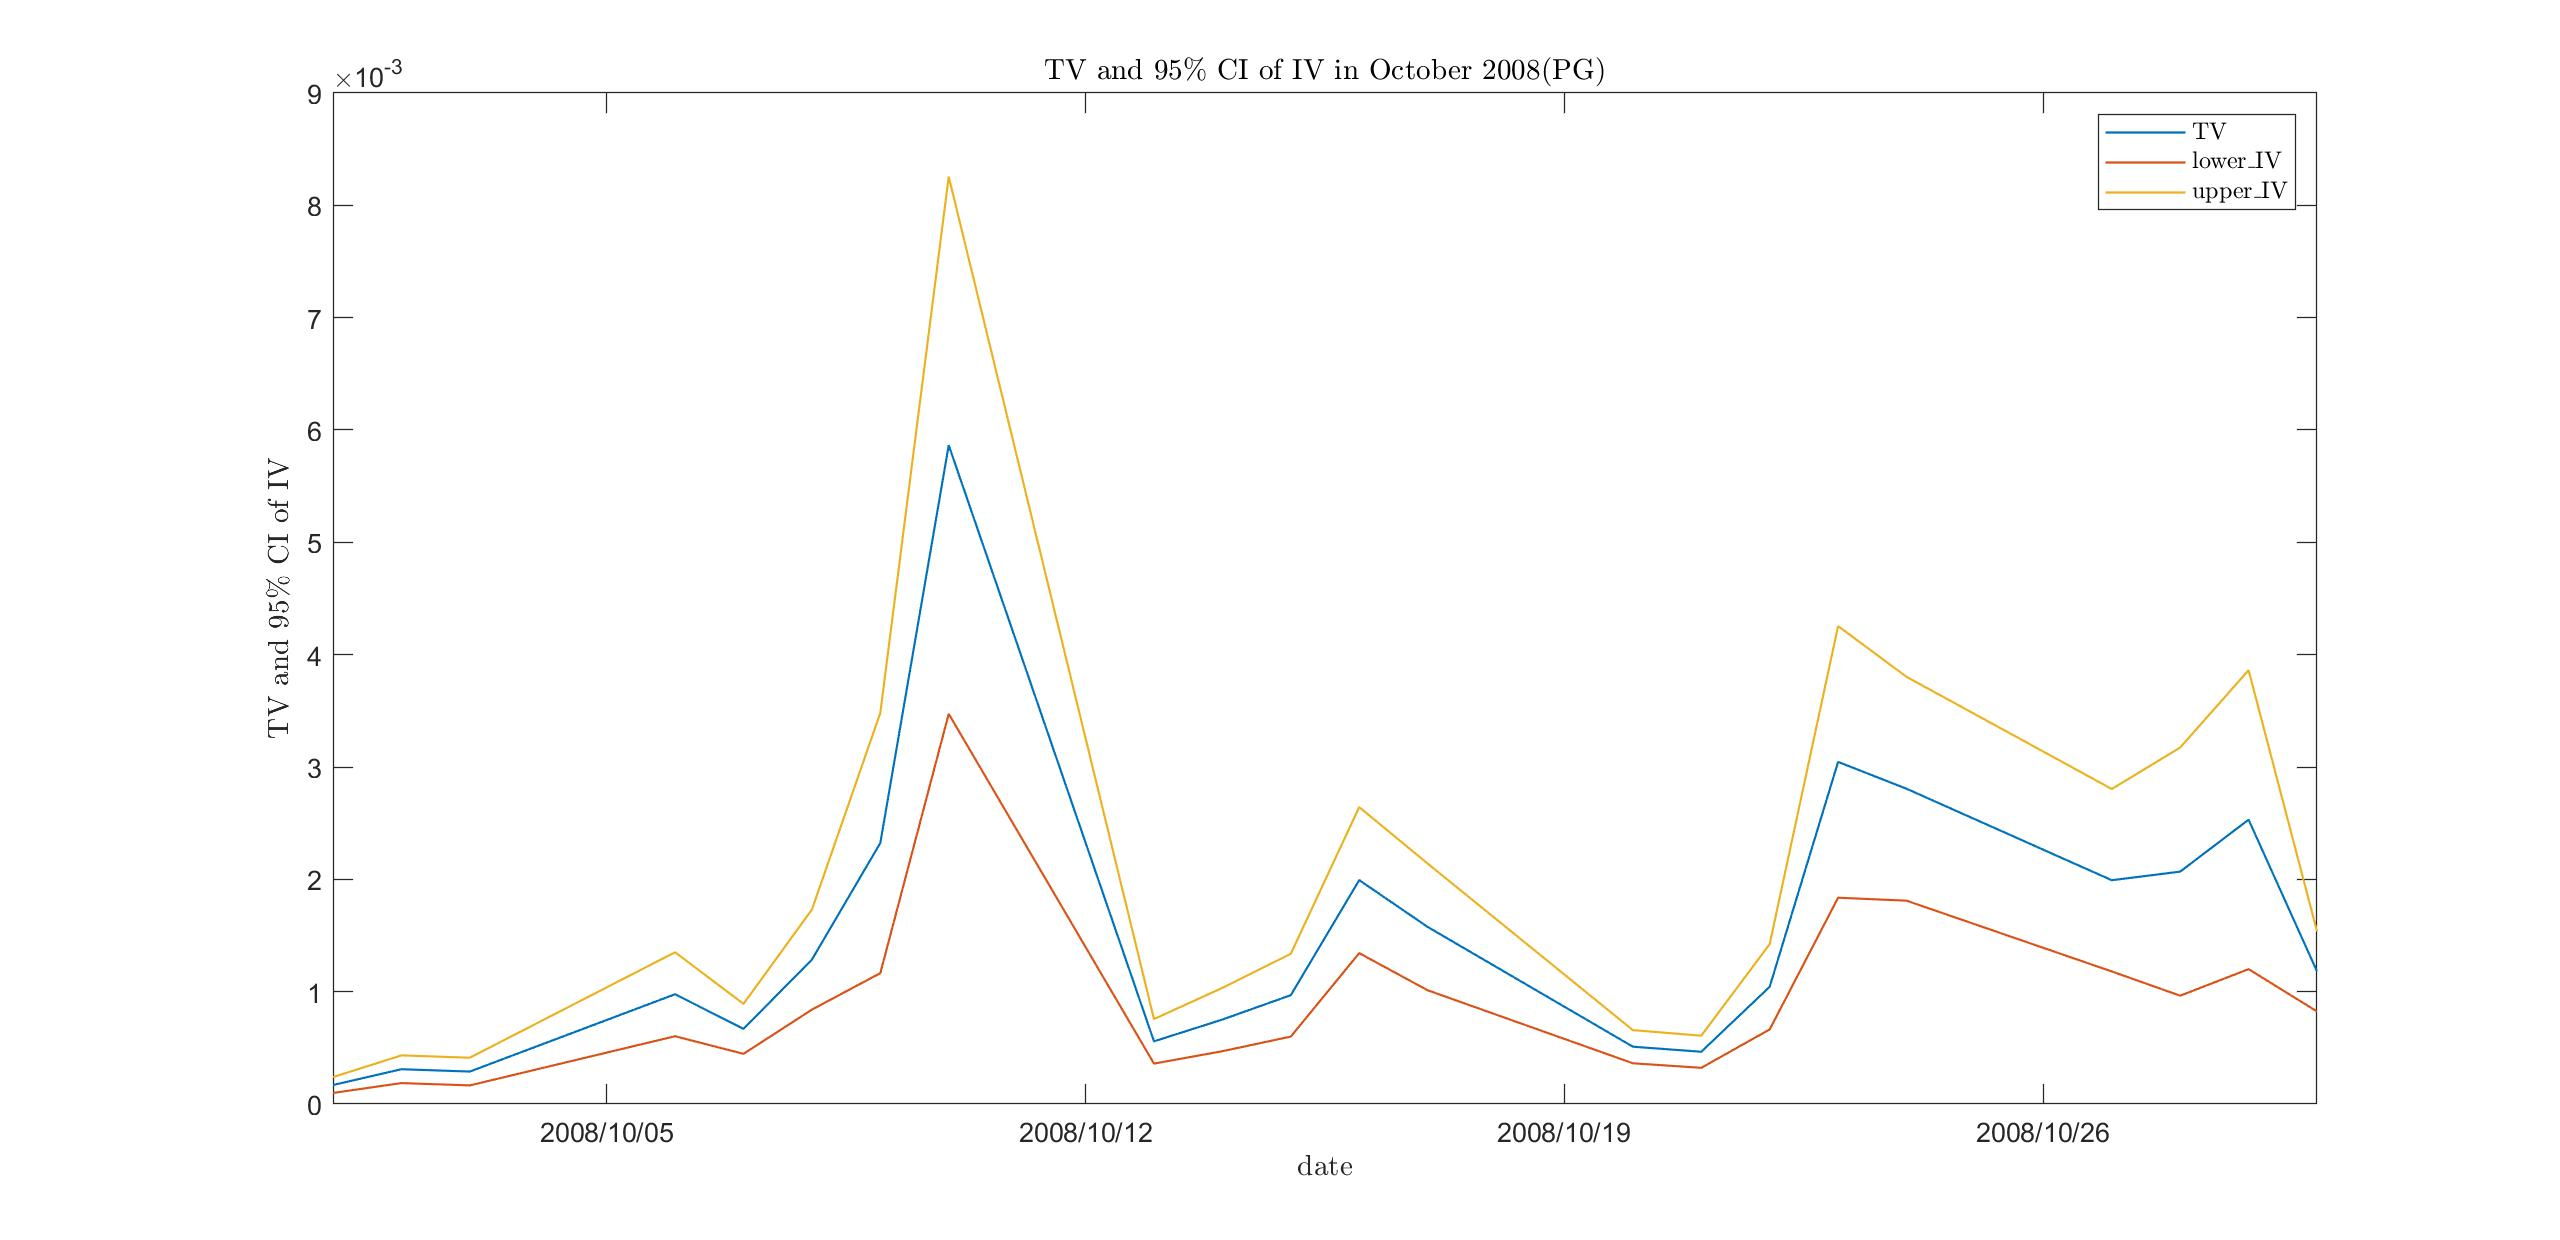
\includegraphics[width=3in]{figures/p3_ex2_e.jpg}
              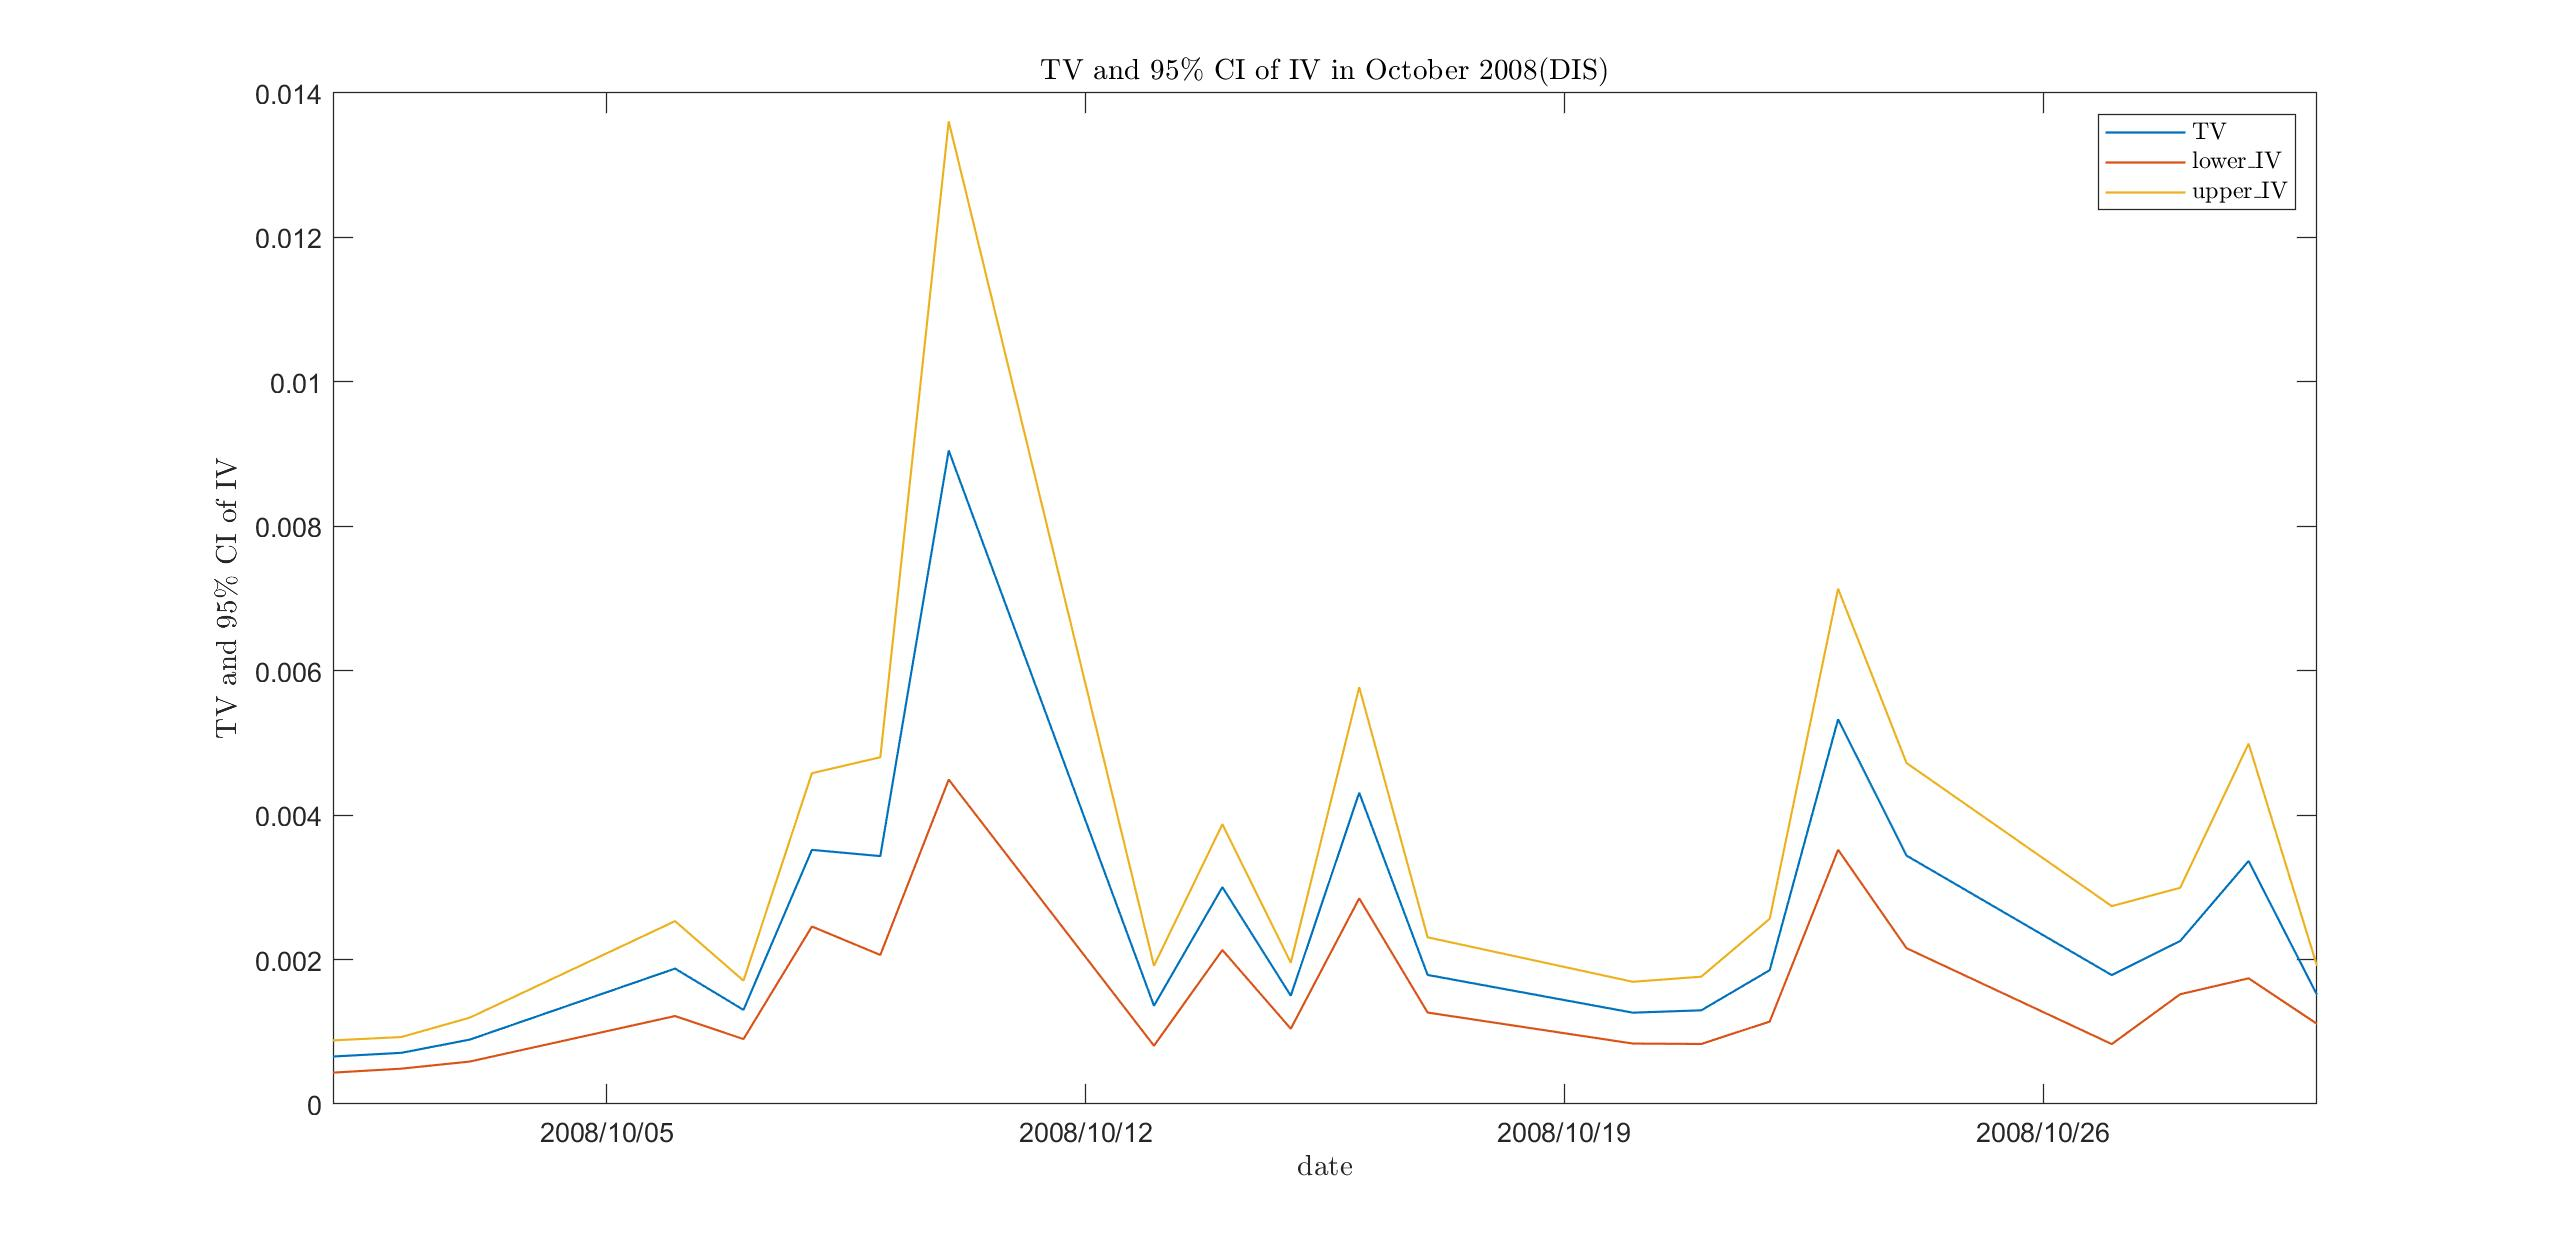
\includegraphics[width=3in]{figures/p3_ex2_e_DIS.jpg}
            \end{minipage}
            }
            \centering
            \caption{TV and IV's estimated confidence interval in October 2008}
\end{figure}

From these figures we can find that, the range of PG and DIS' TV  are (0, 0.006) and (0.0005, 0.009) respectively. The volatility of TV is larger for DIS' TV than PG's. If the TV is a unbiased estimator of IV, then IV's values have 95\% probability fall into the intervals between upper TV and lower TV, which means that we will 95\% IV's value are bounded by the upper value of TV and the lower value of TV. However, if TV is not a unbiased estimator of IV, the percentage that IV fall into the confidence interval estimated by using RV will not equal(or close) to 95\%.  \\


%----2F-----
\item 
 \begin{enumerate}[label=(\roman*)]
    \item If we know the asymptotic distribution of an estimator, then we can get the asymptotic distribution of a function of this estimator by using Delta Method.
    \item By using Delta method, we can easily calculate the asymptotic distribution of the function of estimator, given the asymptotic distribution of this estimator.
    Specifically, if we know the asymptotic distribution of the returns or variance, by using Delta Method, we can get the annual returns or variance's estimator's asymptotic distribution then calculate its confidence interval or other statistic estimators .
    \item Function $g$ in this case is $g(\theta)=100\sqrt{252\theta}$ ($\theta$ in our case is $IV_t$).
    \item By taking derivative of function $g$, we get $g(IV_t)$'=$\frac{300\sqrt{7}}{\sqrt{IV_t}}$.
    \item Since the asymptotic distribution of  $\Delta_n^{-1/2}(TV_t-TV_t)$ is  ~~$\mathcal{N}(0,2QIV_t)$, by using the Delta Method we can get the asymptotic distribution of $\Delta_n^{-1/2}(100\sqrt{252TV_t-252TV_t}$ is ~~$\mathcal{N}(0, 2(g'(IV_t))^2 QIV_t)$, that is  $\mathcal{N}(0, 2*(\frac{300\sqrt{7}}{\sqrt{x}})^2 QIV_t)$.
 \end{enumerate}


%----2G-----
\item The confidence interval for $\Delta_n^{-1/2}(100\sqrt{252TV_t-252IV_t}$ is:
$$CI(100\sqrt{252\times IV_t},1-\alpha)=[100 \sqrt{252TV_t} \pm q_z(\frac{\alpha}{2}) \times 100 \frac{3\sqrt{7}}{\sqrt{TV_t}} \sqrt{2\Delta_t \hat{QIV_t}} ]$$

%----2G-----
\item Here are the plots of annual TV and 95\% confidence intervals.
 \begin{figure}[H]
           \subfigure{
           \begin{minipage}[l]{1\linewidth}
           \centering
             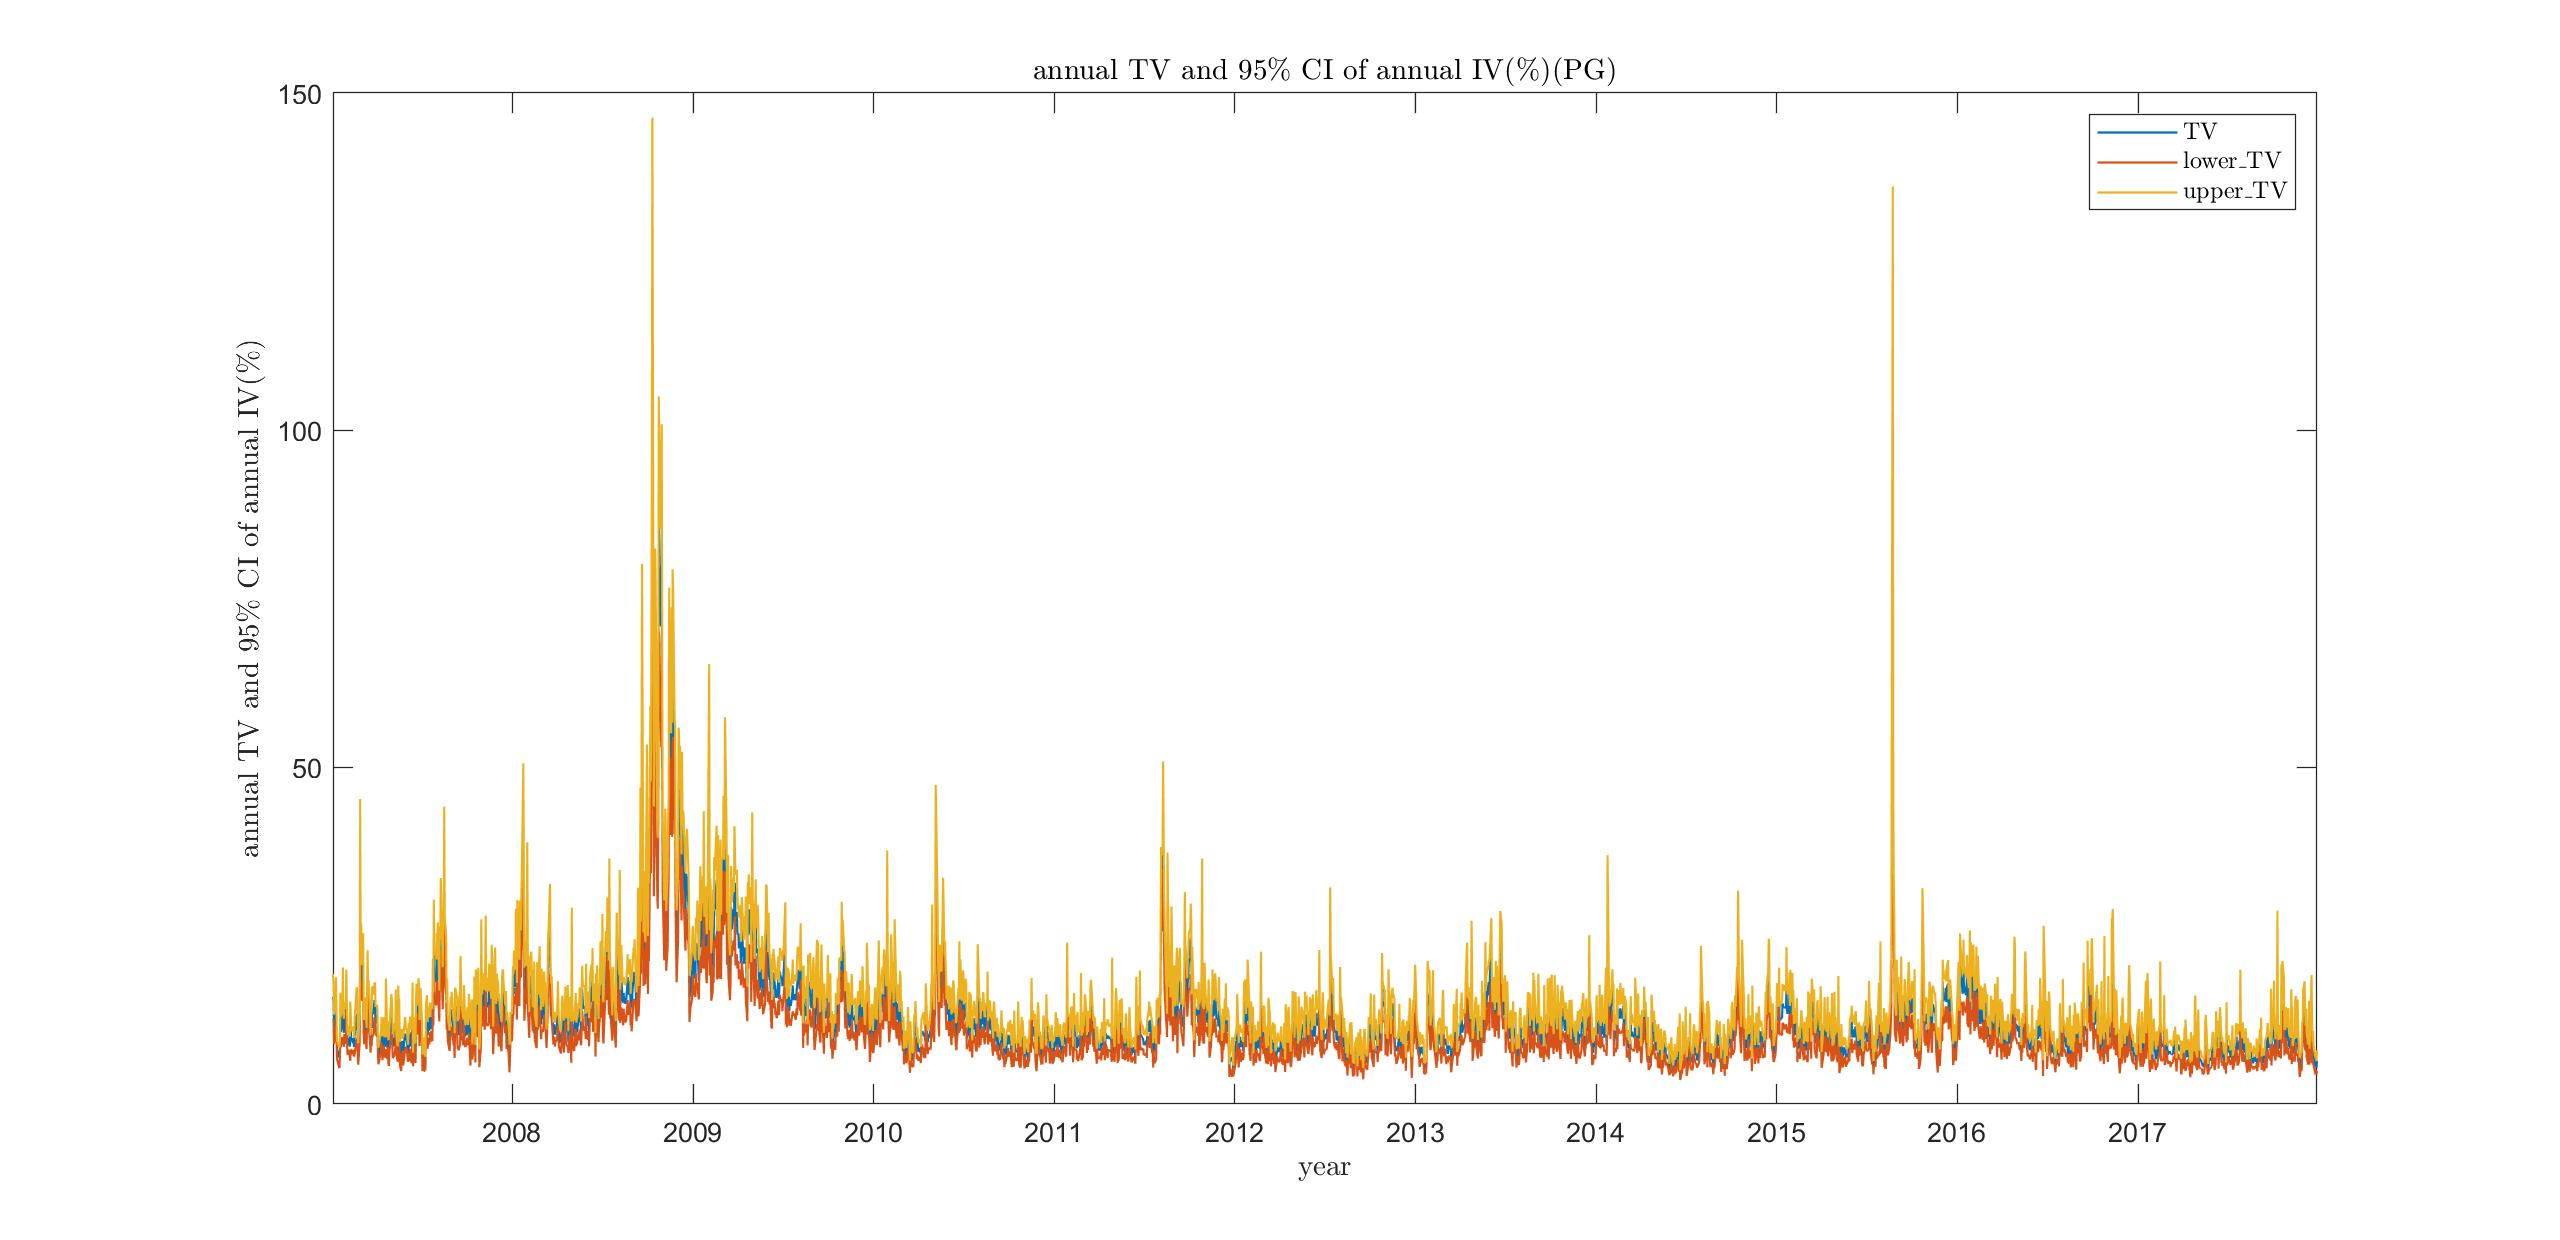
\includegraphics[width=3in]{figures/p3_ex2_h1.jpg}
              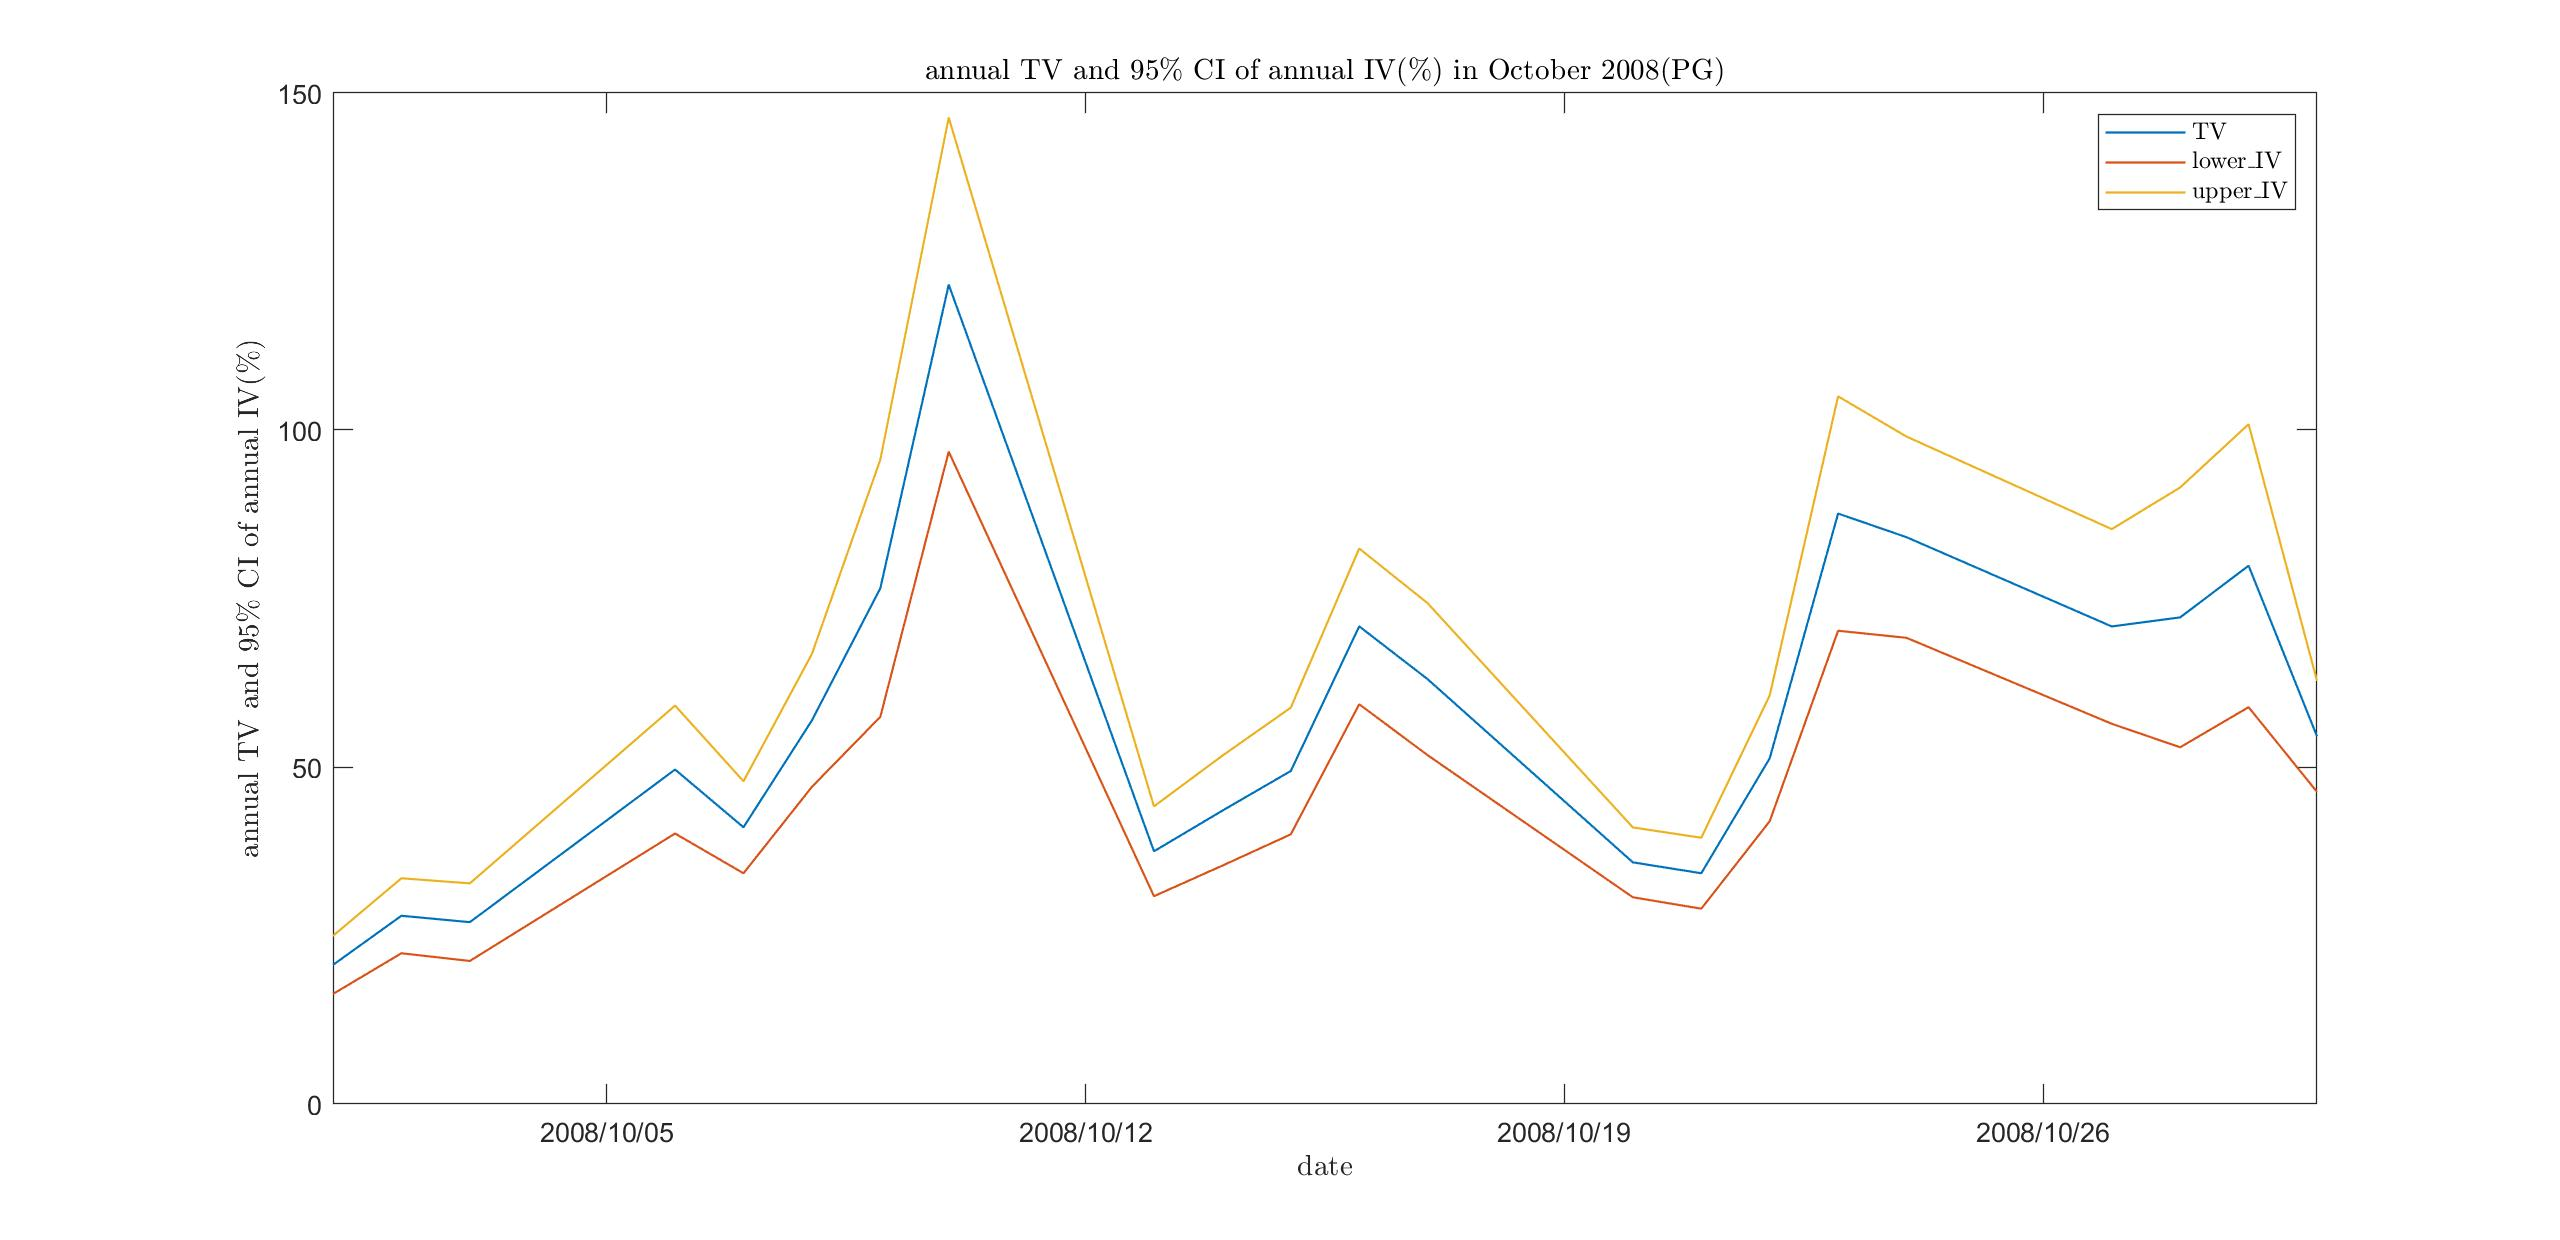
\includegraphics[width=3in]{figures/p3_ex2_h3.jpg}
            \end{minipage}
            }
               \subfigure{
           \begin{minipage}[l]{1\linewidth}
           \centering
             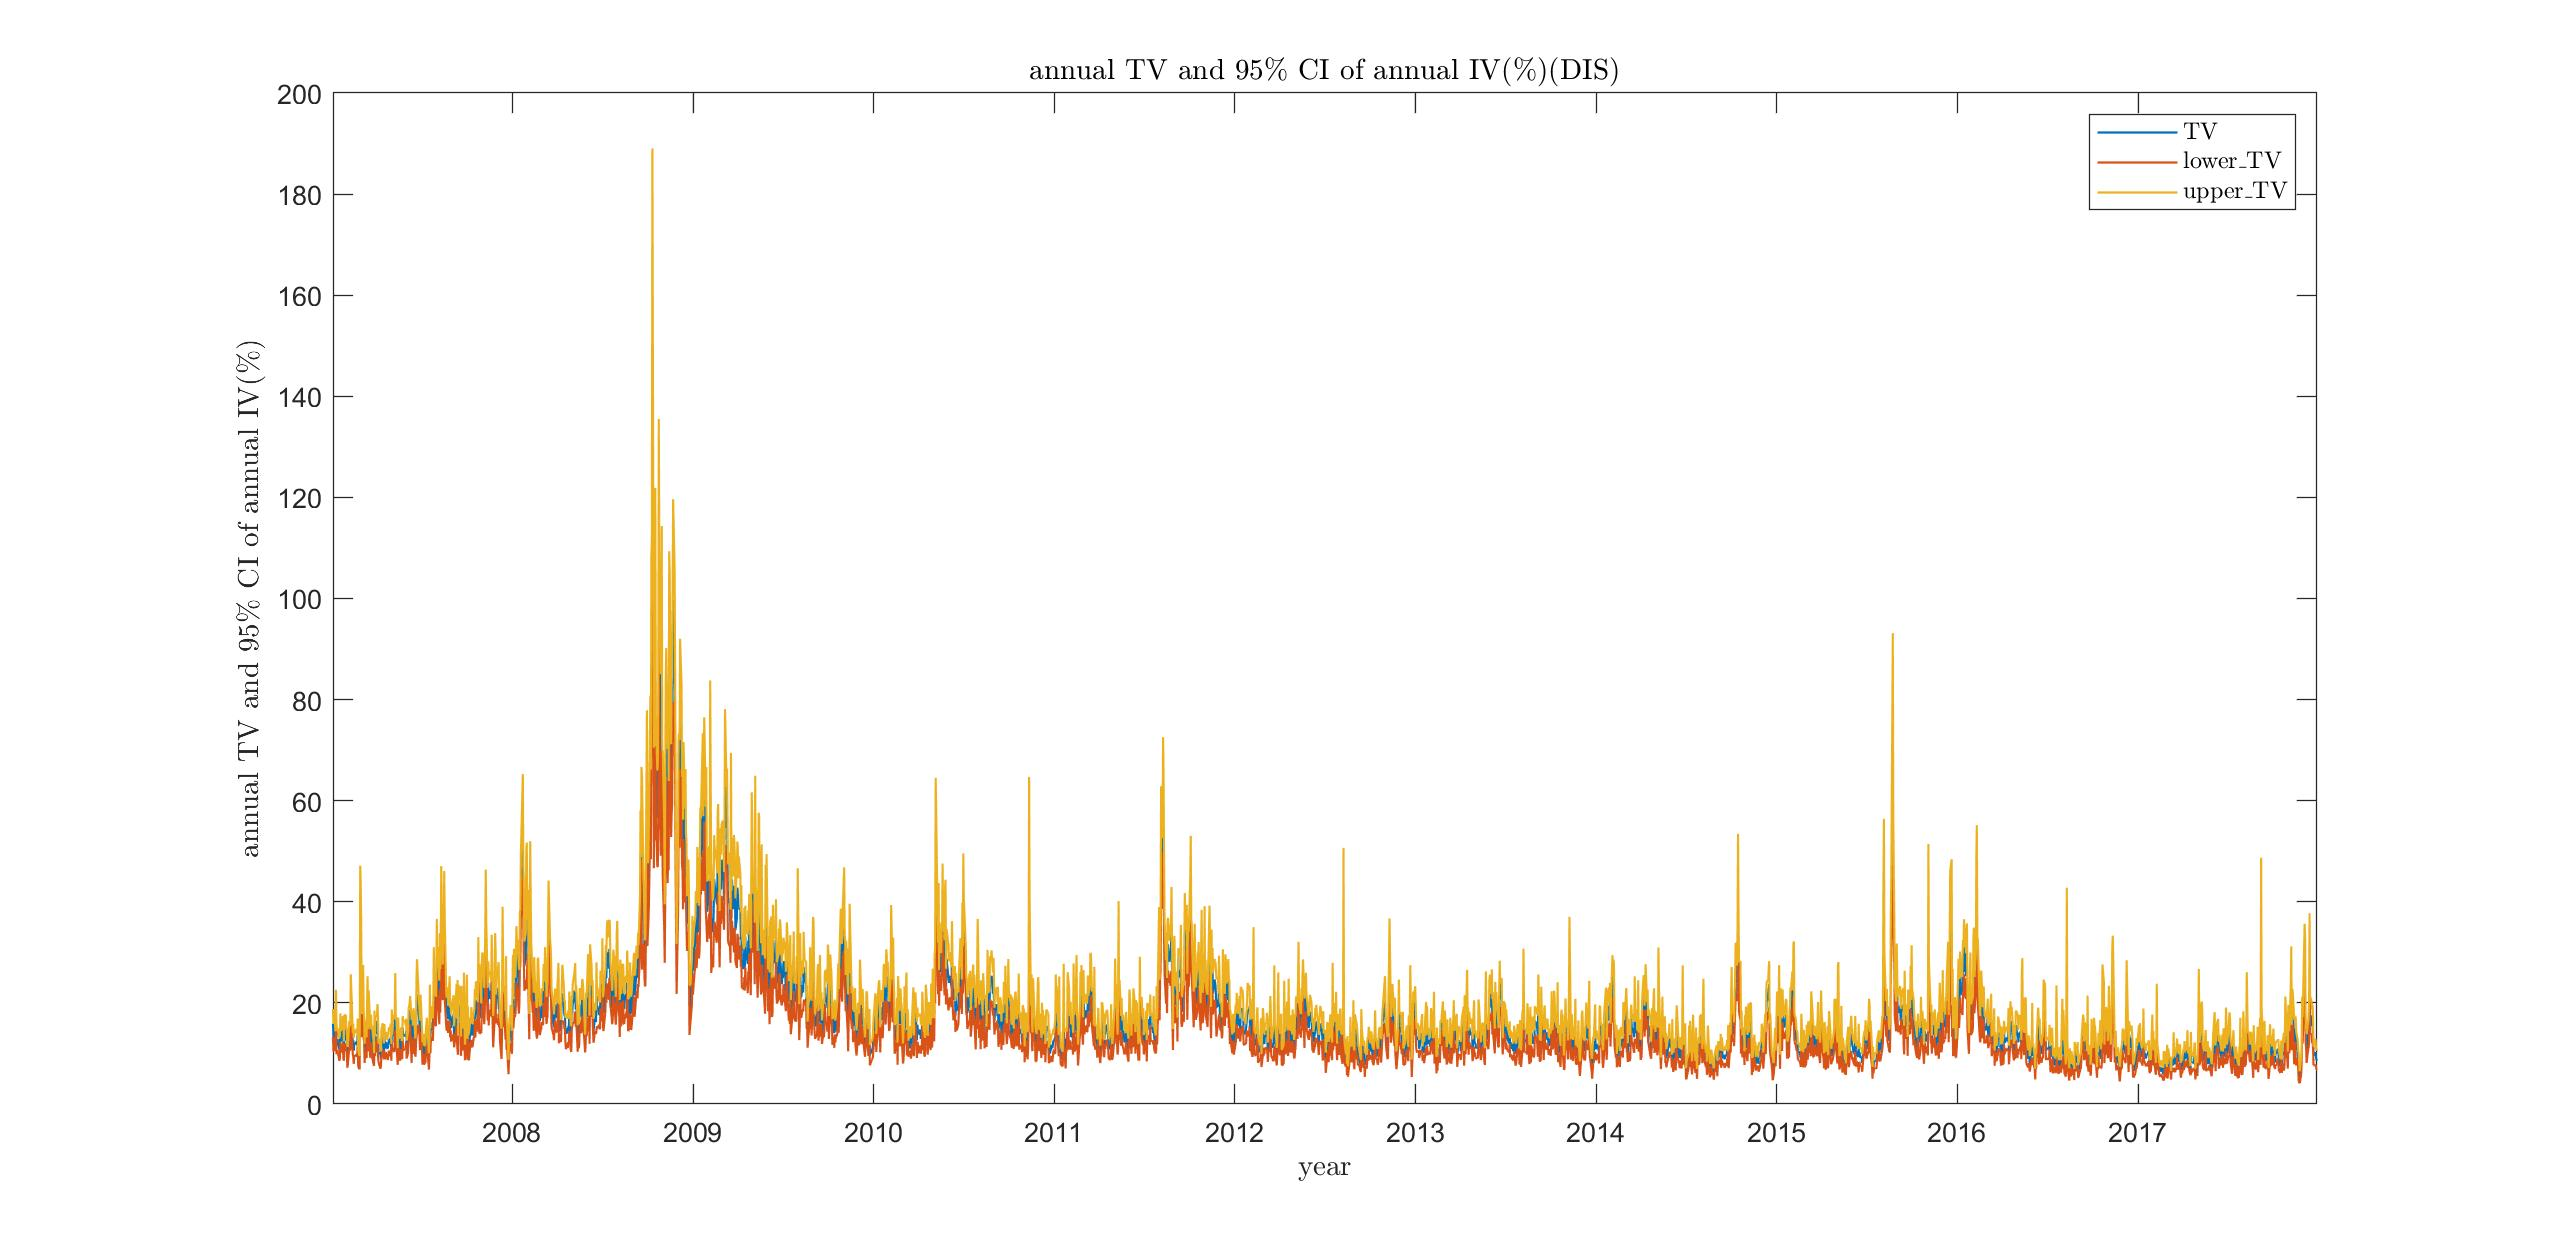
\includegraphics[width=3in]{figures/p3_ex2_h1_DIS.jpg}
              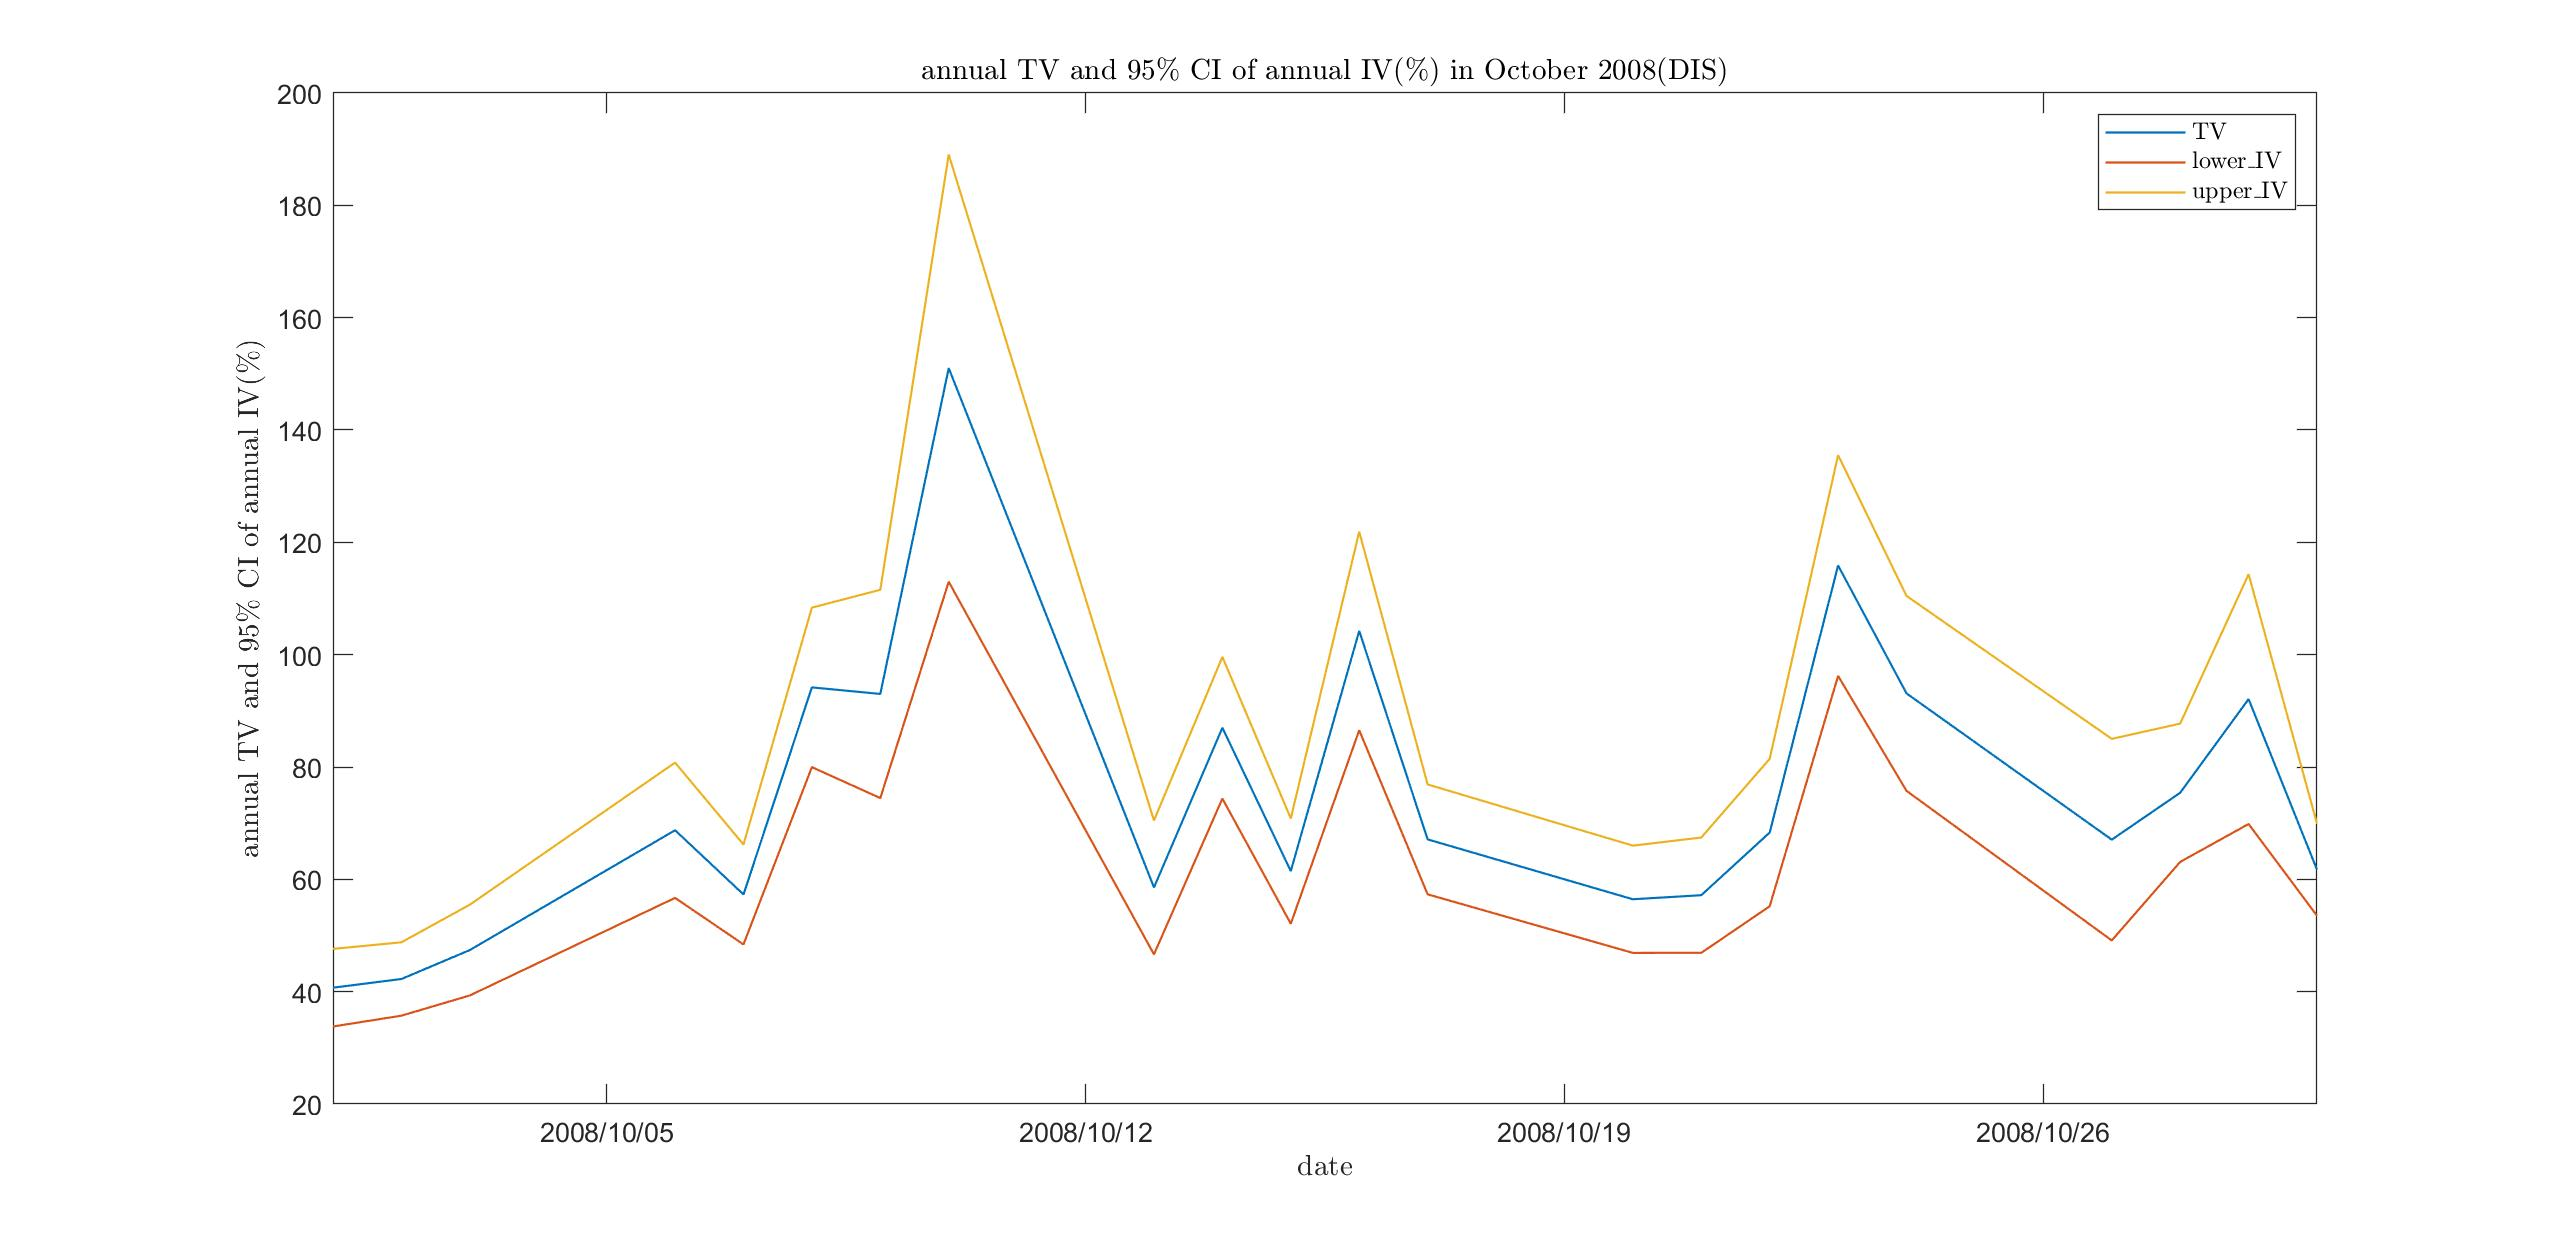
\includegraphics[width=3in]{figures/p3_ex2_h3_DIS.jpg}
            \end{minipage}
            }
            \centering
            \caption{Estimated confidence interval for PG and DIS}
\end{figure}

As we can see from the figures (focus on October 2008) that, PG and DIS' annual TV have similar shape, they both have small fluctuations on 10 Oct. 2008 and 16 Oct. 2008 and 23 Oct. 2008 and 29 Oct. 2008. According to the figure, we can find that the upper bound and the lower bound of confidence interval have the similar shape of TVt, which may means that we have calculate the correct confidence interval(at lease the shape of confidence interval is right). If the TVt is a unbiased estimator of IVt, then IVt's values have 95\% probability fall into the intervals between upper TVt and lower TVt, that is, the percentage that IVt fall into the confidence interval estimated by using RVt will not equal(or close) to 95\%.\\

The \textbf{MATLAB} code for function to calculate adjusted volatility with different frequency:
   \lstinputlisting{scripts/p3_ex2_PG.m}
\end{enumerate}
\newpage

%---------------------------------------------
\section*{Exercise 3}
  \begin{enumerate}[label=\textbf{(\Alph*)}]
%----A-----
 \item  To construct stochastic variance process  $C_{t,i}$:
  \begin{enumerate}[label=(\roman*)]
  	\item Construct a series number from the standard normal distribution;
  	\item Compute each  $C_{t,i}$ by iteration;
  \end{enumerate}
 
Here is the plot of time series prices:
        \begin{figure}[H]
            \centering
            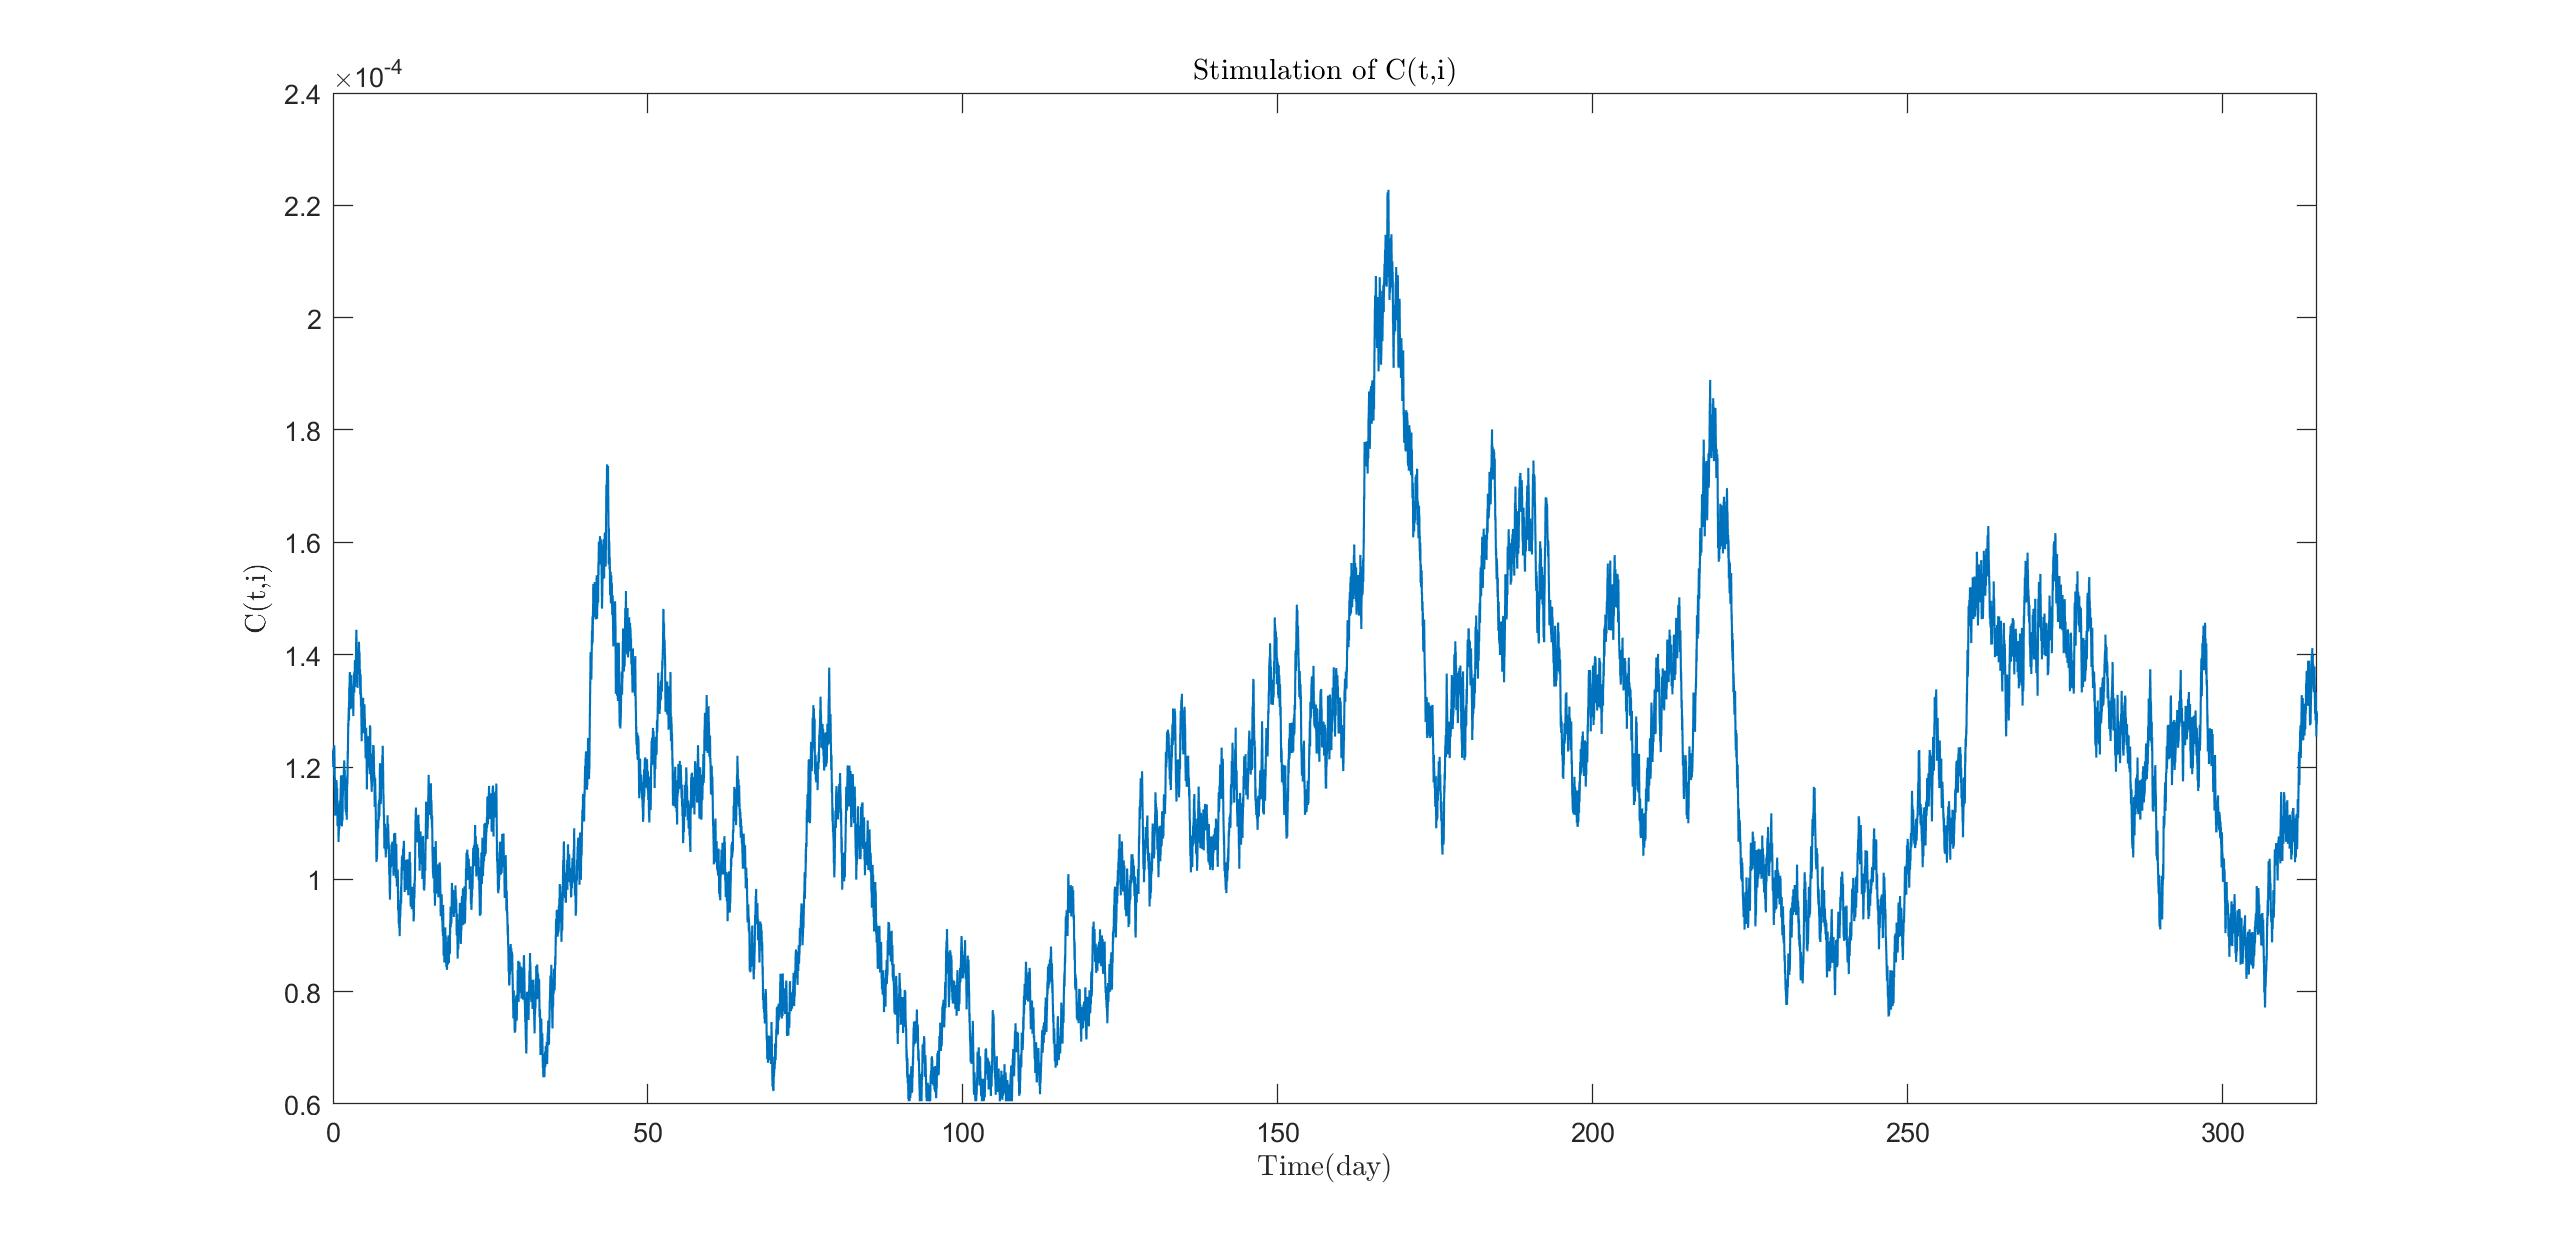
\includegraphics[width=10cm]{figures/p3_ex3_a.jpg}
            \caption{Stimulation of $C_{t,i}$}
        \end{figure}
The \textbf{MATLAB} code:
   \lstinputlisting{functions/JD_sv_ct.m}
   ~~\\ 
	      
%----B-----
\item  
\begin{enumerate}[label=(\roman*)]
    \item $IV_t$ is the volatility of log returns' variance $C_t$ at day t.
    \item Since we do not have a continuous ${C_t}$ to calculate $IV_t$, we need to use an Euler discretization scheme, that is we will simulate the model at a very high frequency and sum all the small interval areas( $\Delta_n \times C_{t,i}$) to estimate the integral of $C_t$.
\end{enumerate}

%----C-----
\item The follow are the volatility plots for $C_t$ ($IV_t$):
\begin{figure}[H]
            \centering
            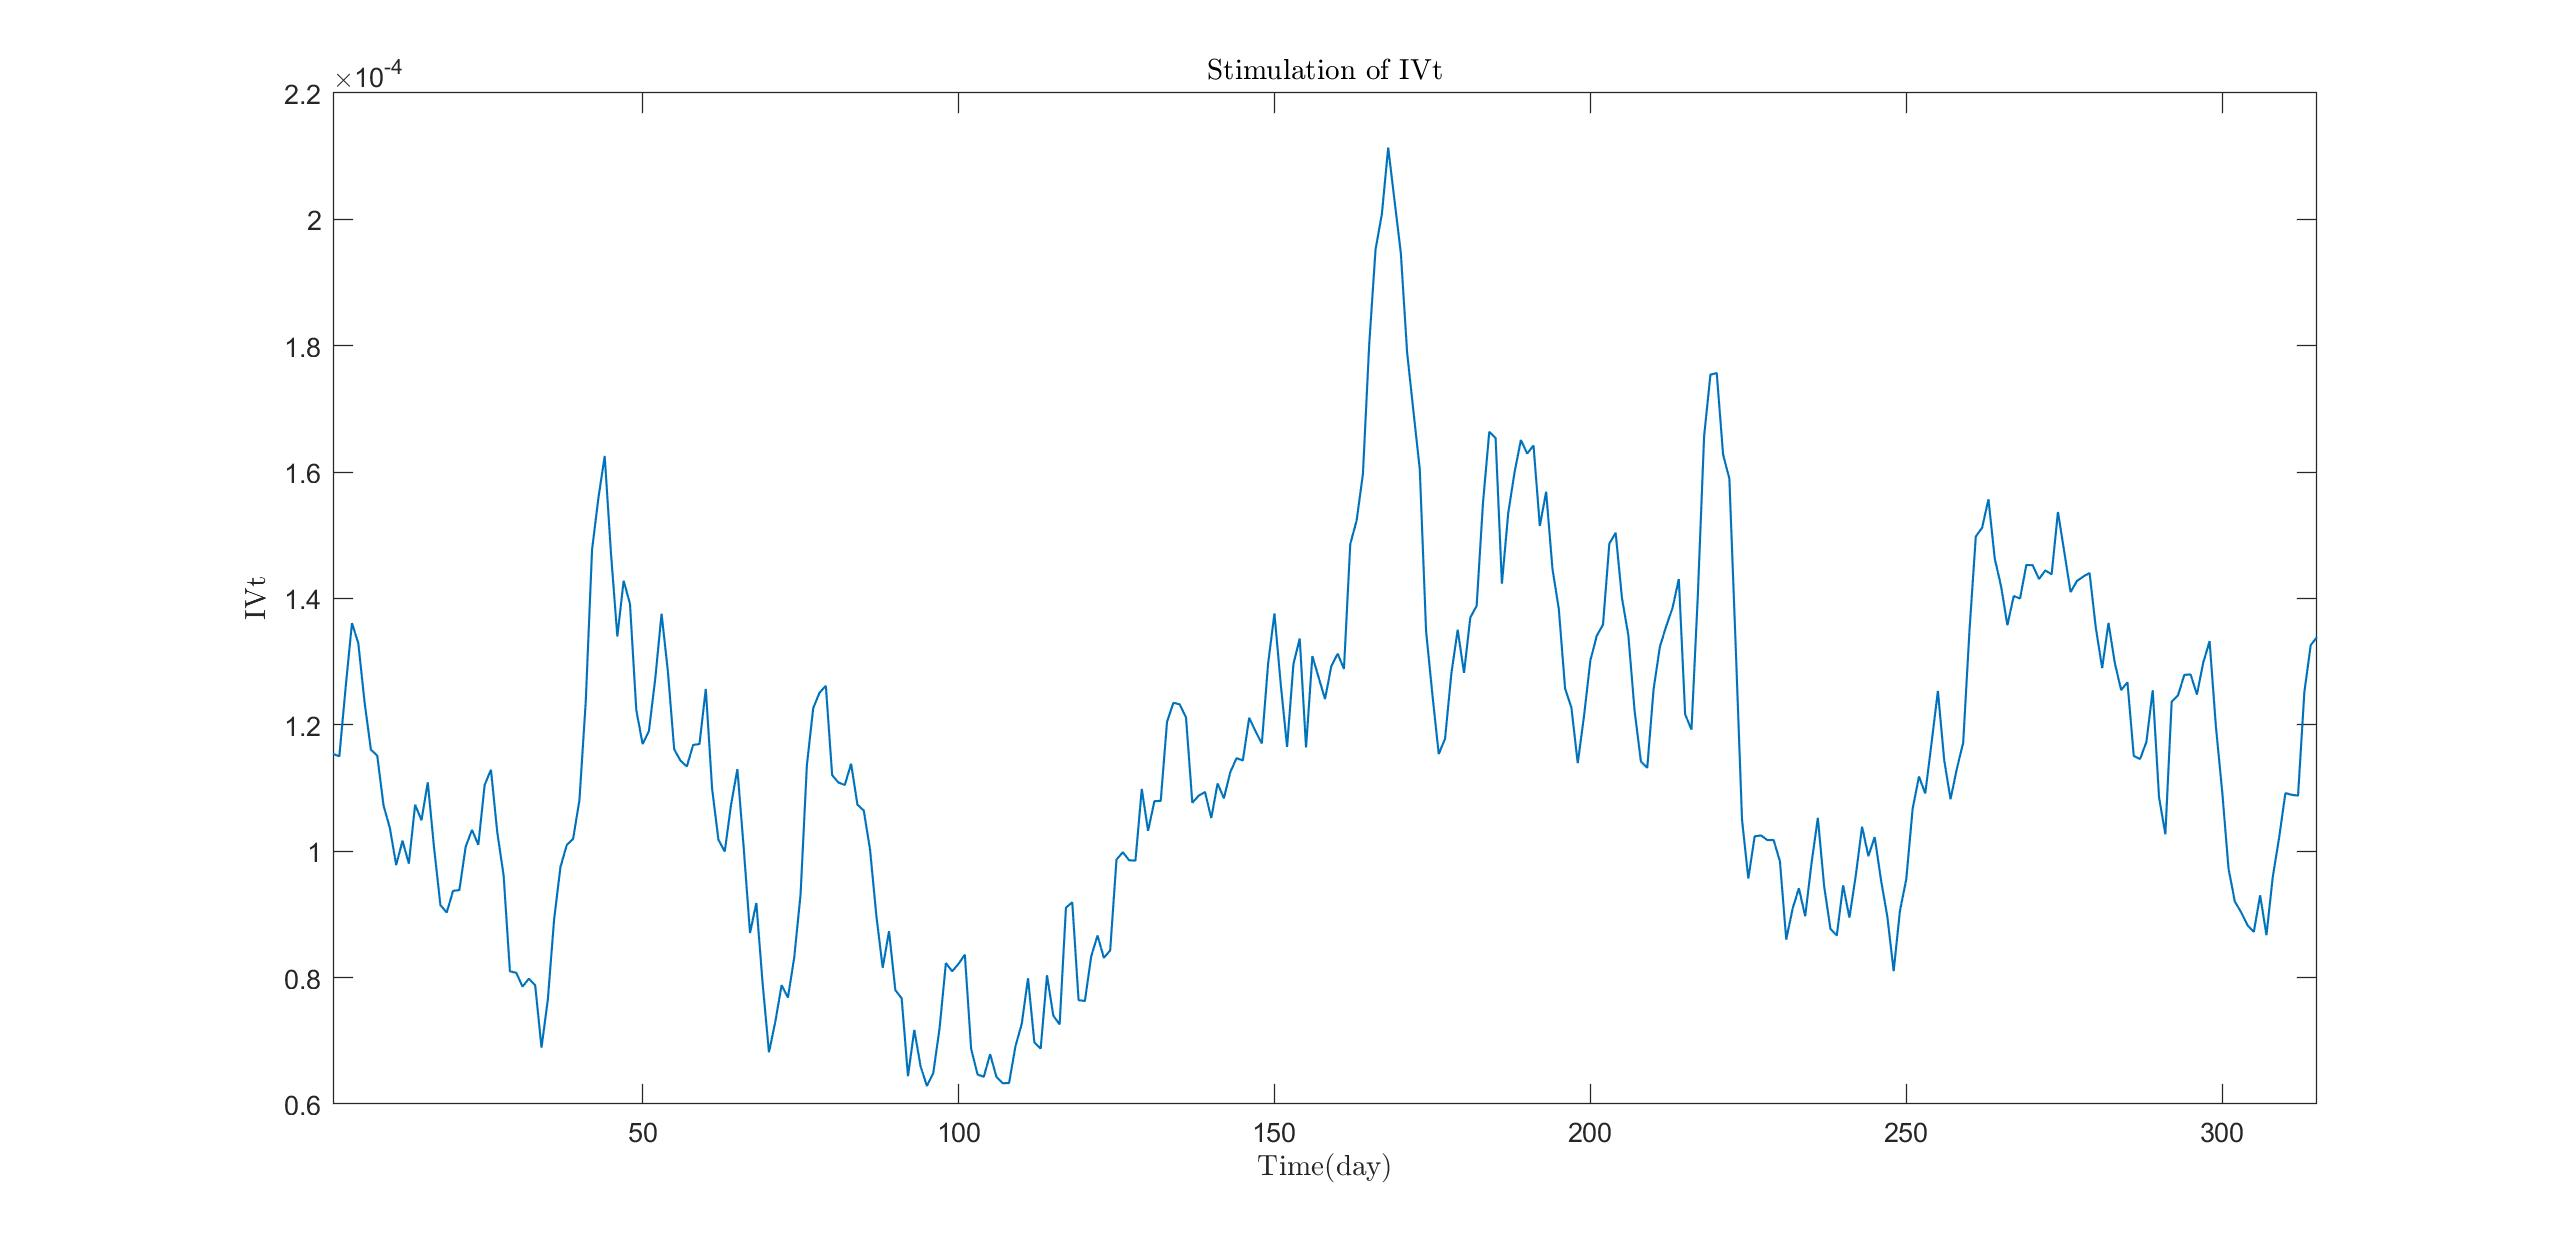
\includegraphics[width=10cm]{figures/p3_ex3_c.jpg}
            \caption{Estimated $IV_t$}
           
        \end{figure}
        
From the figure, we can find the range of $IV_t$ is (0.6$\times$ $10^{-6}$, 0.2$\times$ $10^{-6}$ ). At time around 20, 200 and 250, there are large jump of $IV_t$. Comparing with the plot of $C_{t,i}$ we can find that $IV_t$ have a similar shape of $C_{t,i}$ and the curve of $IV_t$ is smoother than the curve of $C_{t,i}$. The method we use to estimate $IV_t$ is efficient. \\

%----D-----
\item Here are the plots of $IV_t$ and $RV_t$.
      \begin{figure}[H]
            \centering
            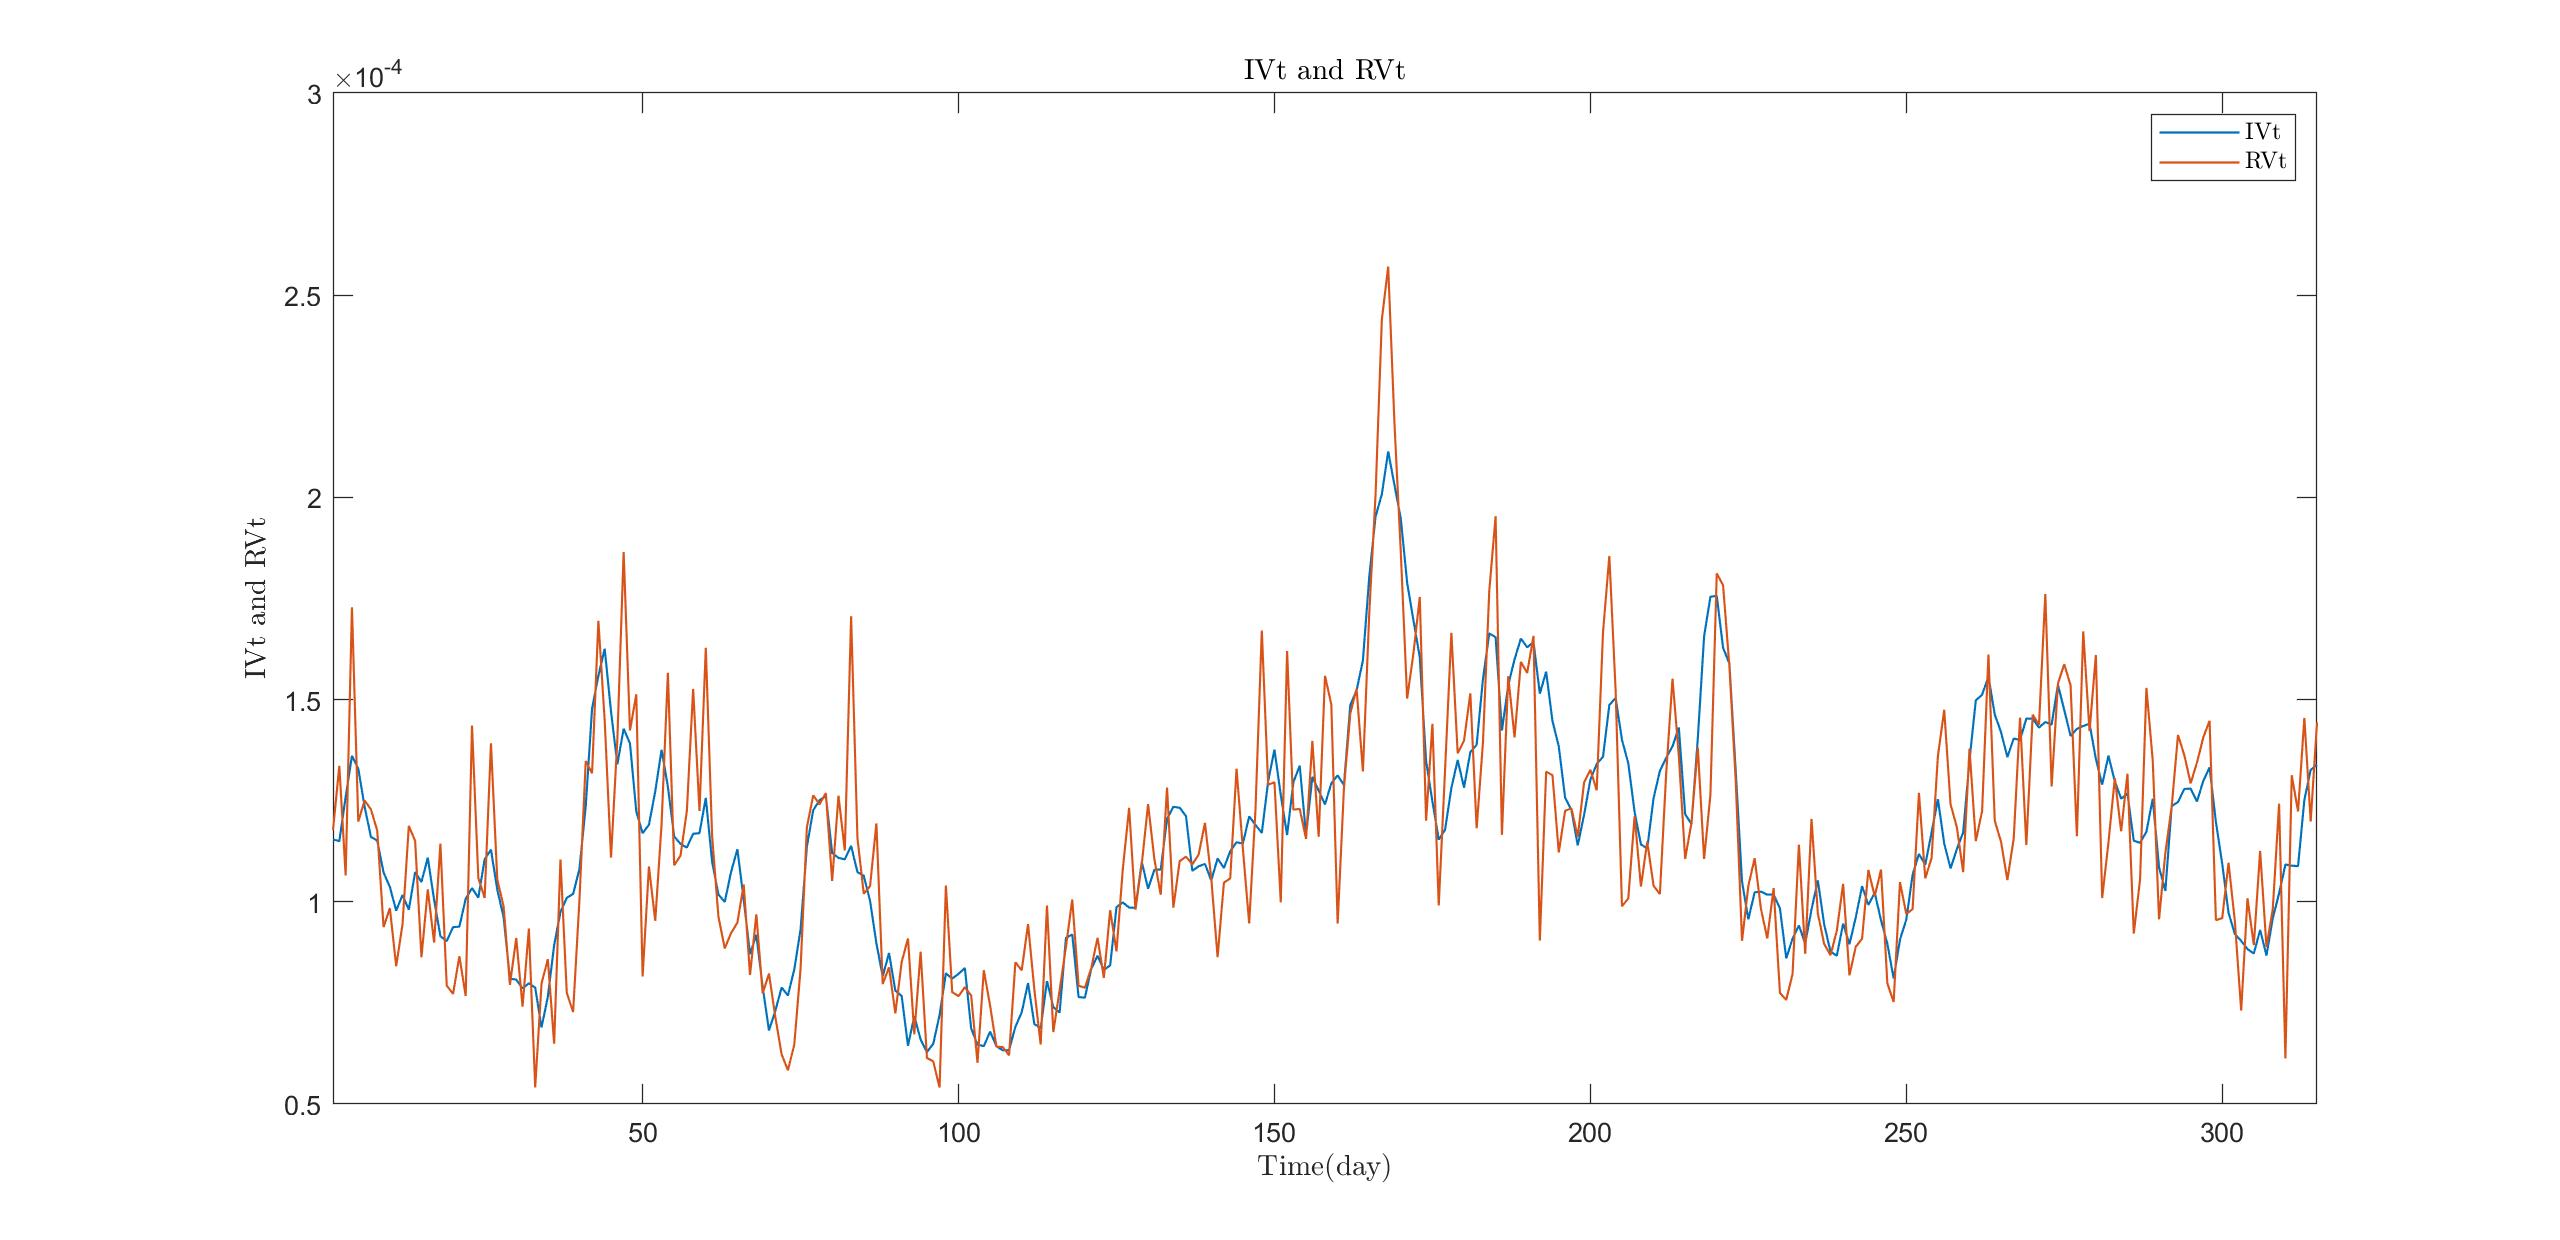
\includegraphics[width=10cm]{figures/p3_ex3_d.jpg}
            \caption{$IV_t$ and $RV_t$}
           
        \end{figure}
        
From this figure we can find that, RV and IV have the similar shape but RV shows more volatility than IV. The range of RV and IV are (0.5 $\times$ $10^{-4}$, 2.6$\times$ $10^{-4}$) and (0.6$\times$ $10^{-4}$,2.1 $\times$ $10^{-4}$) respectively. RV has show all the movements of IV, which means that RV here is a good estimator of IV.\\

%----E-----
\item We can get the estimated 95\% confidence interval by using QIV's estimator $\hat{QIV}$ and IV's estimator RV. Here is the plot.
\begin{figure}[H]
            \centering
            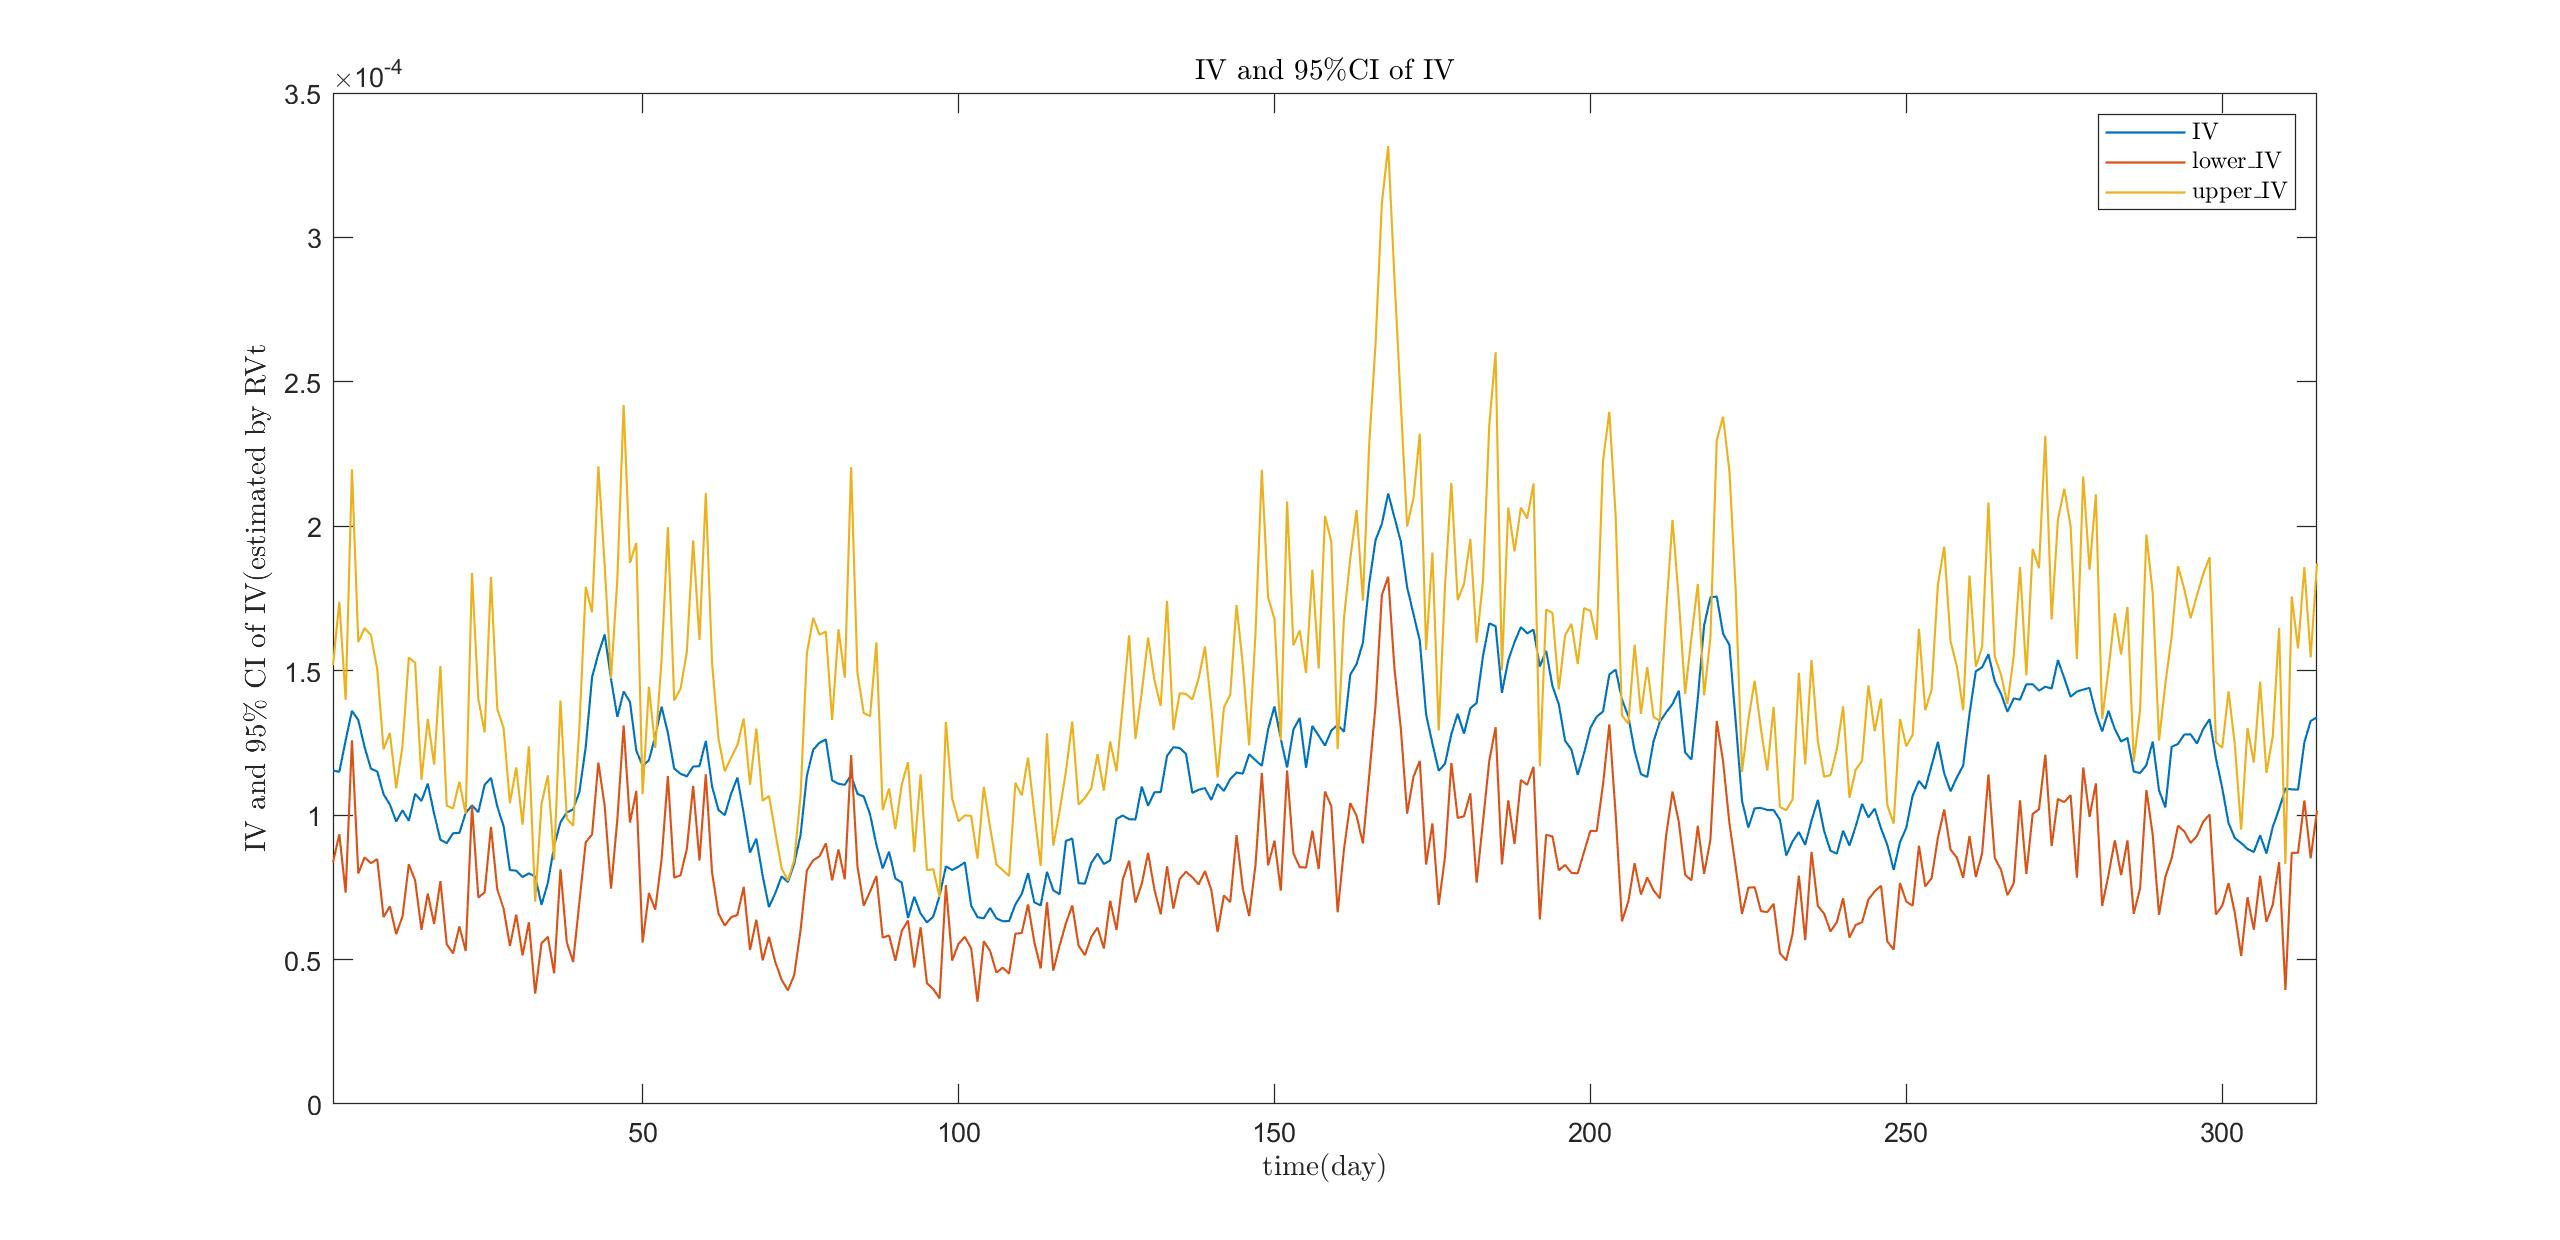
\includegraphics[width=10cm]{figures/p3_ex3_e.jpg}
            \caption{$IV_t$ and Estimated Confidence Interval}
           
        \end{figure}
From the figure, we can find that both the lower bound and upper bound of IV have the similar shape of Iv. For most of the sample of IV, IV's values are bounded by estimated confidence interval. According to the figure, we can say that using RV as an estimator of IV to calculate the confidence interval of IV works well.

%----F-----
\item 
\begin{enumerate}[label=(\roman*)]
    \item The number of days that $IV_t$'s values within the confidence interval is 298;
    \item The average cover rate is 94.6\%;
    \item the average cover rate is close to the expected 95\%.
\end{enumerate}
   
%----G-----
\item Here is the figure of stock price with jump.
\begin{figure}[H]
            \centering
            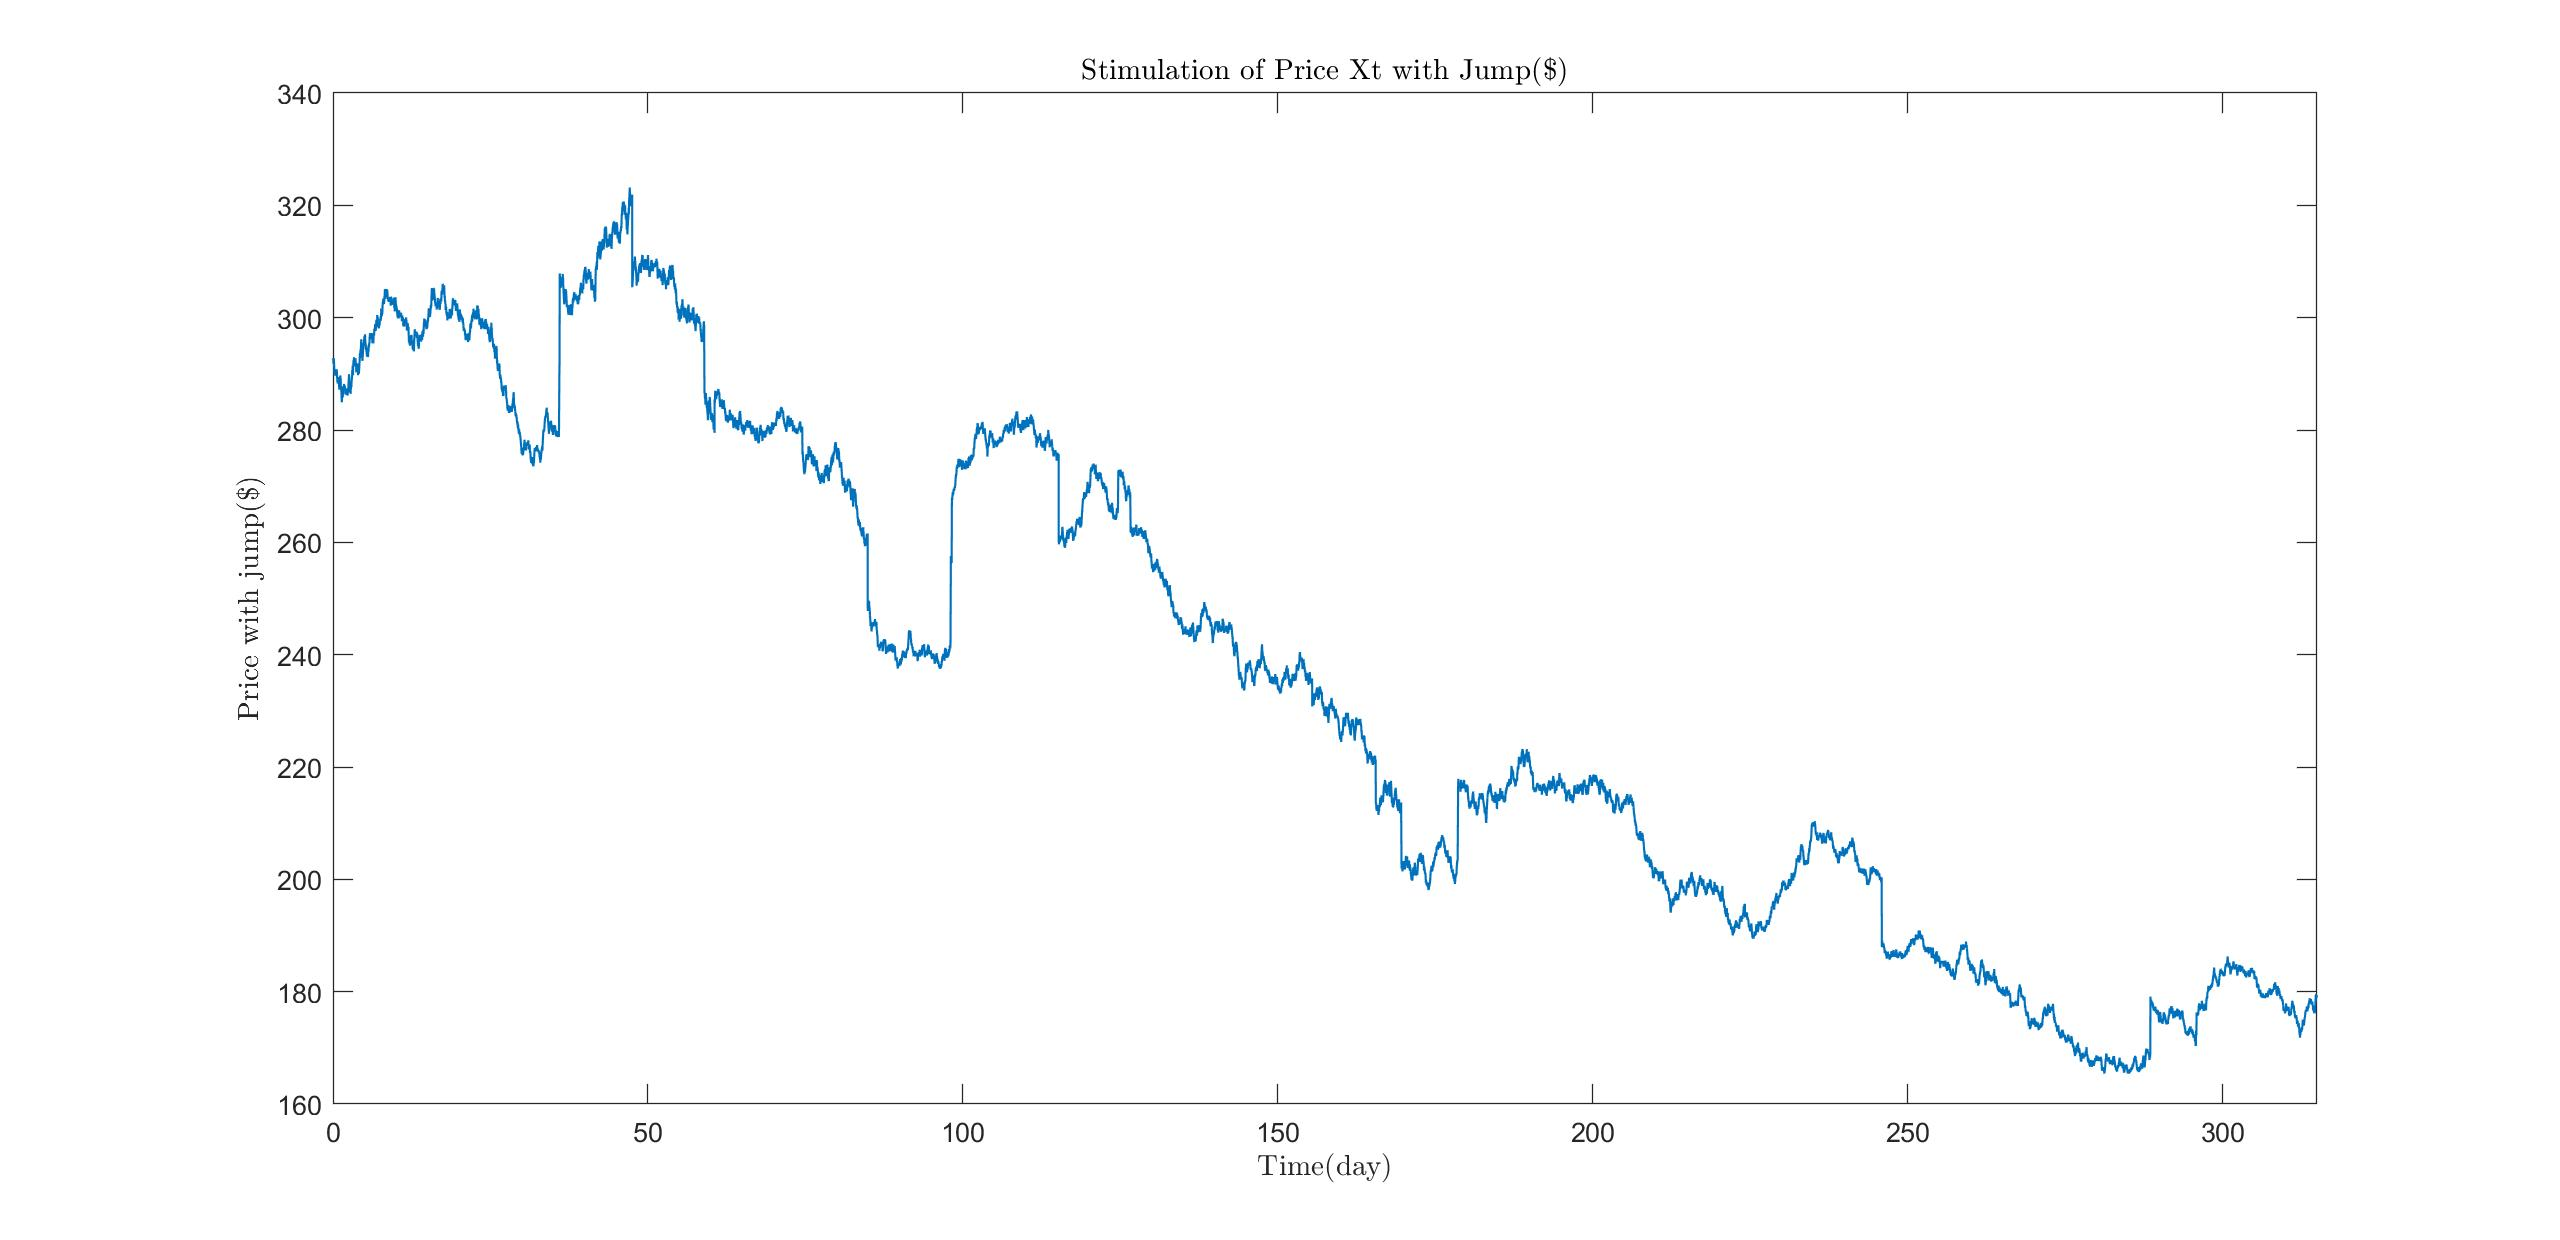
\includegraphics[width=10cm]{figures/p3_ex3_g.jpg}
            \caption{Stimulated stock price with jump}
        \end{figure}
 
The \textbf{MATLAB} code:
   \lstinputlisting{functions/jump1.m} 
        
%----H-----
\item Here is the figure of estimated confidence interval of annual IV based on the asymptotic theory.
\begin{figure}[H]
            \centering
            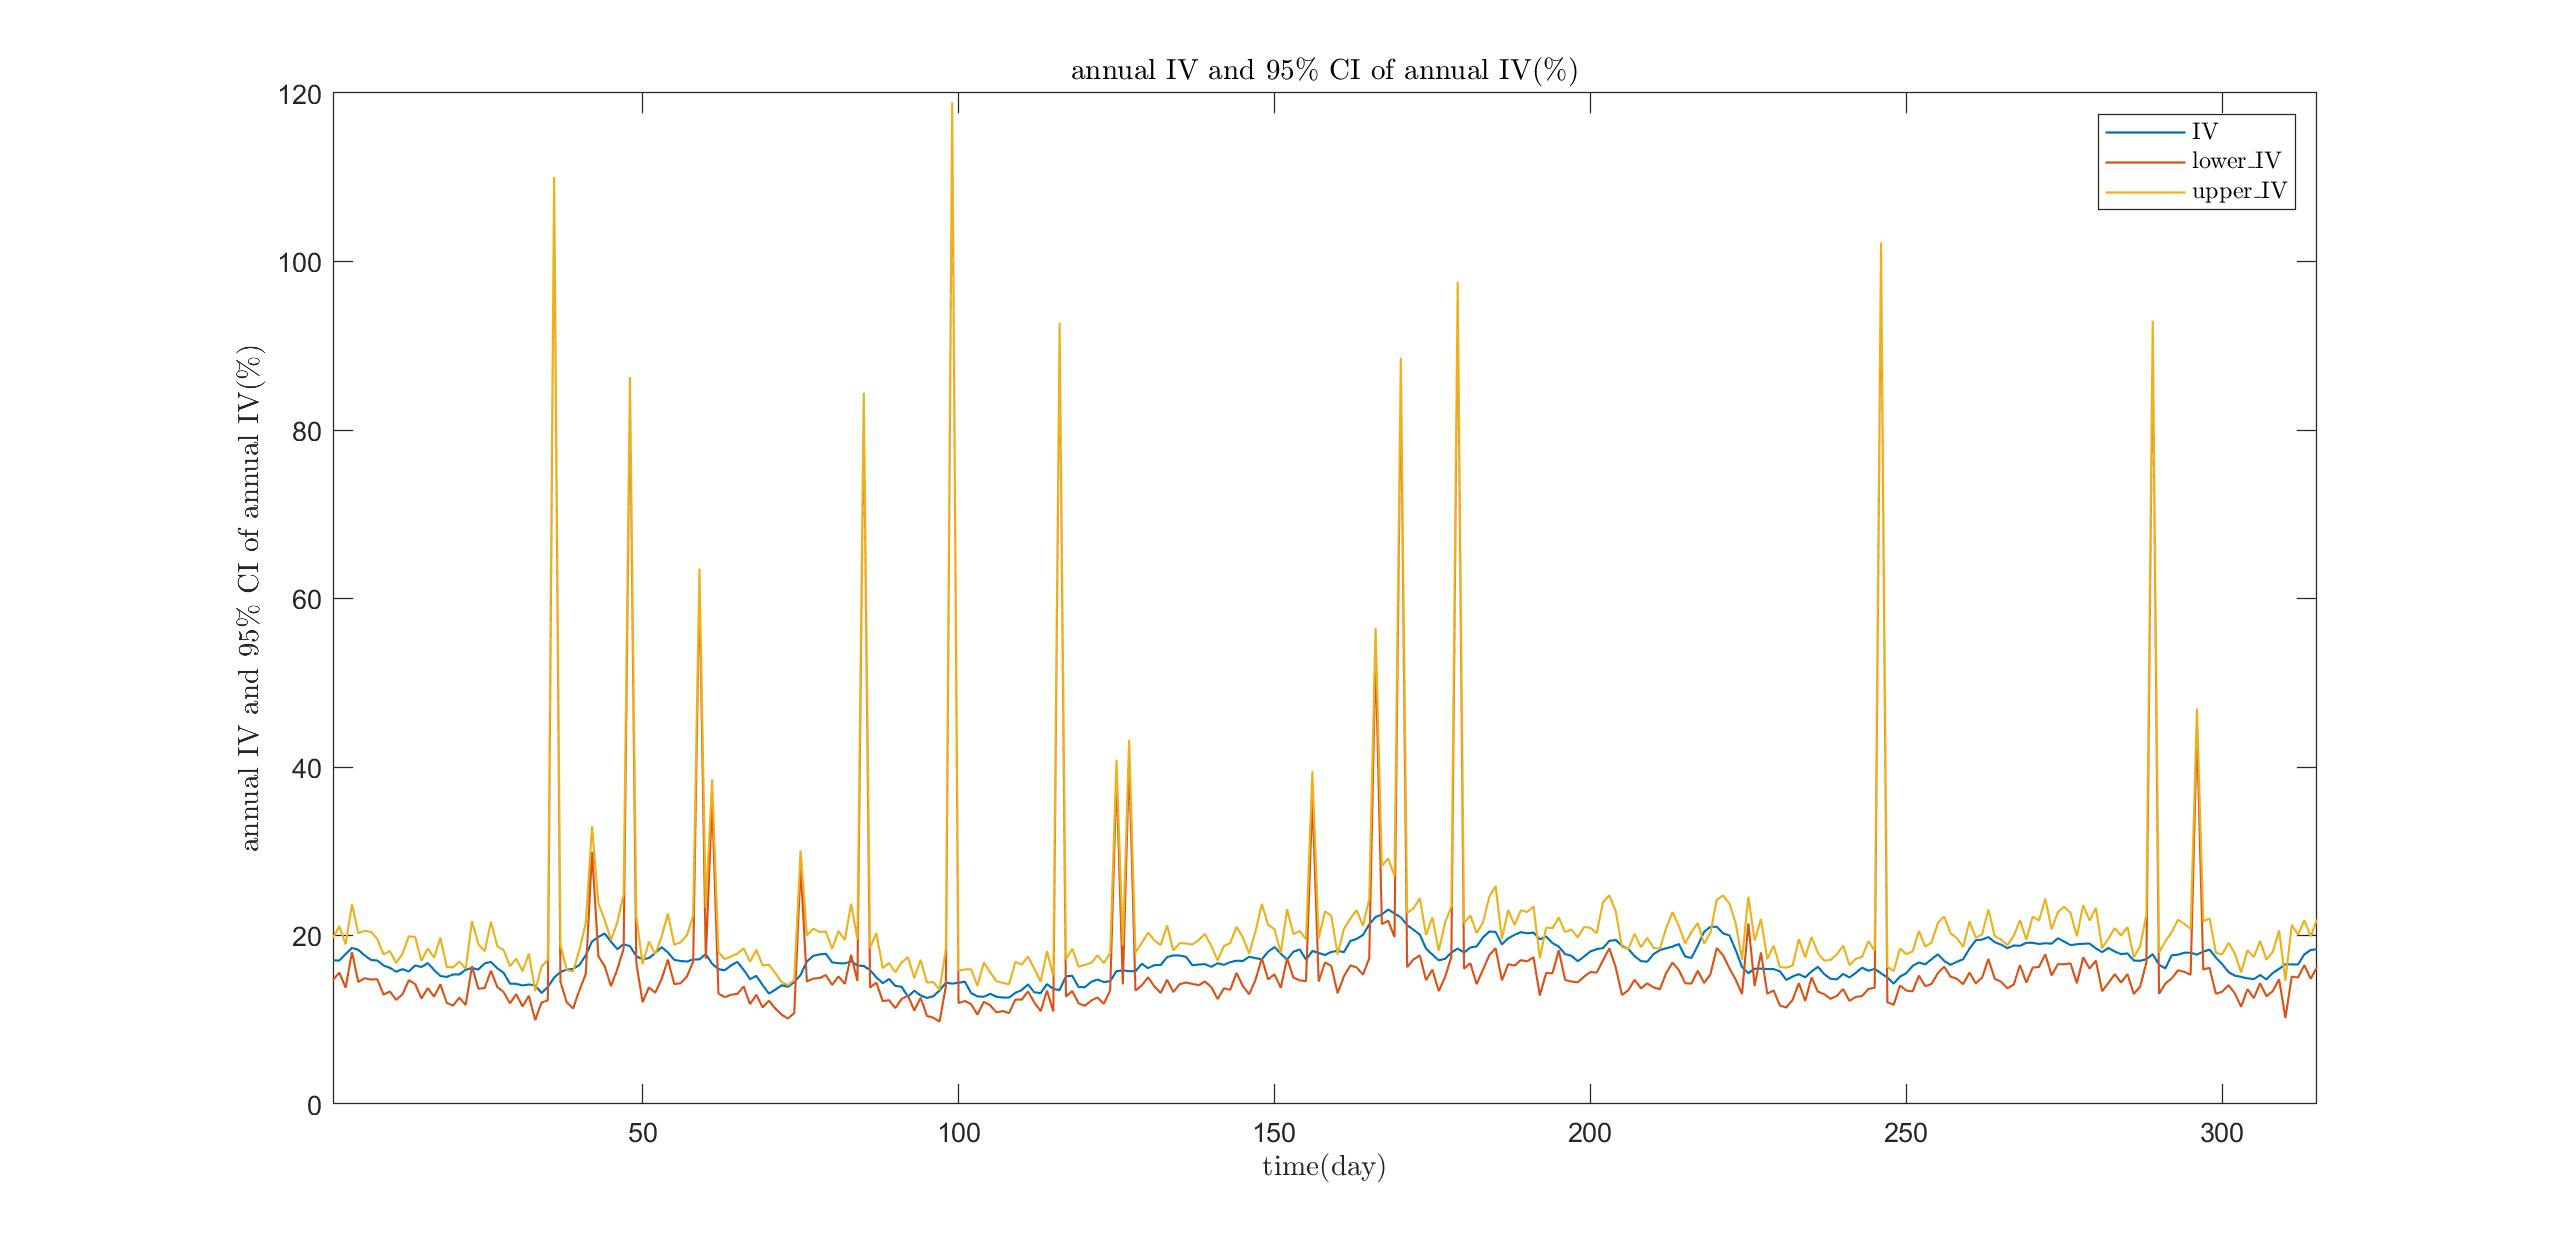
\includegraphics[width=10cm]{figures/p3_ex3_h.jpg}
            \caption{Estimated confidence interval of annual IV(\%)}
        \end{figure}
\begin{enumerate}[label=(\roman*)]
    \item The coverage rate of the confidence interval is 88.25\%;
    \item The cover rate when price with jump is smaller than the case when price does not include jumps.
    \item The cover rate is what I expected, since when there is jump in stock price, RV will never be a unbiased estimator of IV. So, if we use the biased estimator to calculate the confidence interval of IV, then the confidence interval will not be a good estimated confidence interval and the cover rate will decrease.
    \item When we fail to account the jump returns, we may regard RV as a unbiased estimator of IV. However, RV is no longer a unbiased estimator for IV now. This incorrect assumption will affect the confidence interval we calculated: the estimated confidence interval will also bias from the ``true'' confidence interval, which mean the probability that Iv falls within the estimated confidence interval will not equal(or close) to confidence level anymore.\\
    
\end{enumerate}

%----I-----
\item Here is the figure of estimated confidence interval of annual IV based on the asymptotic theory.
\begin{figure}[H]
            \centering
            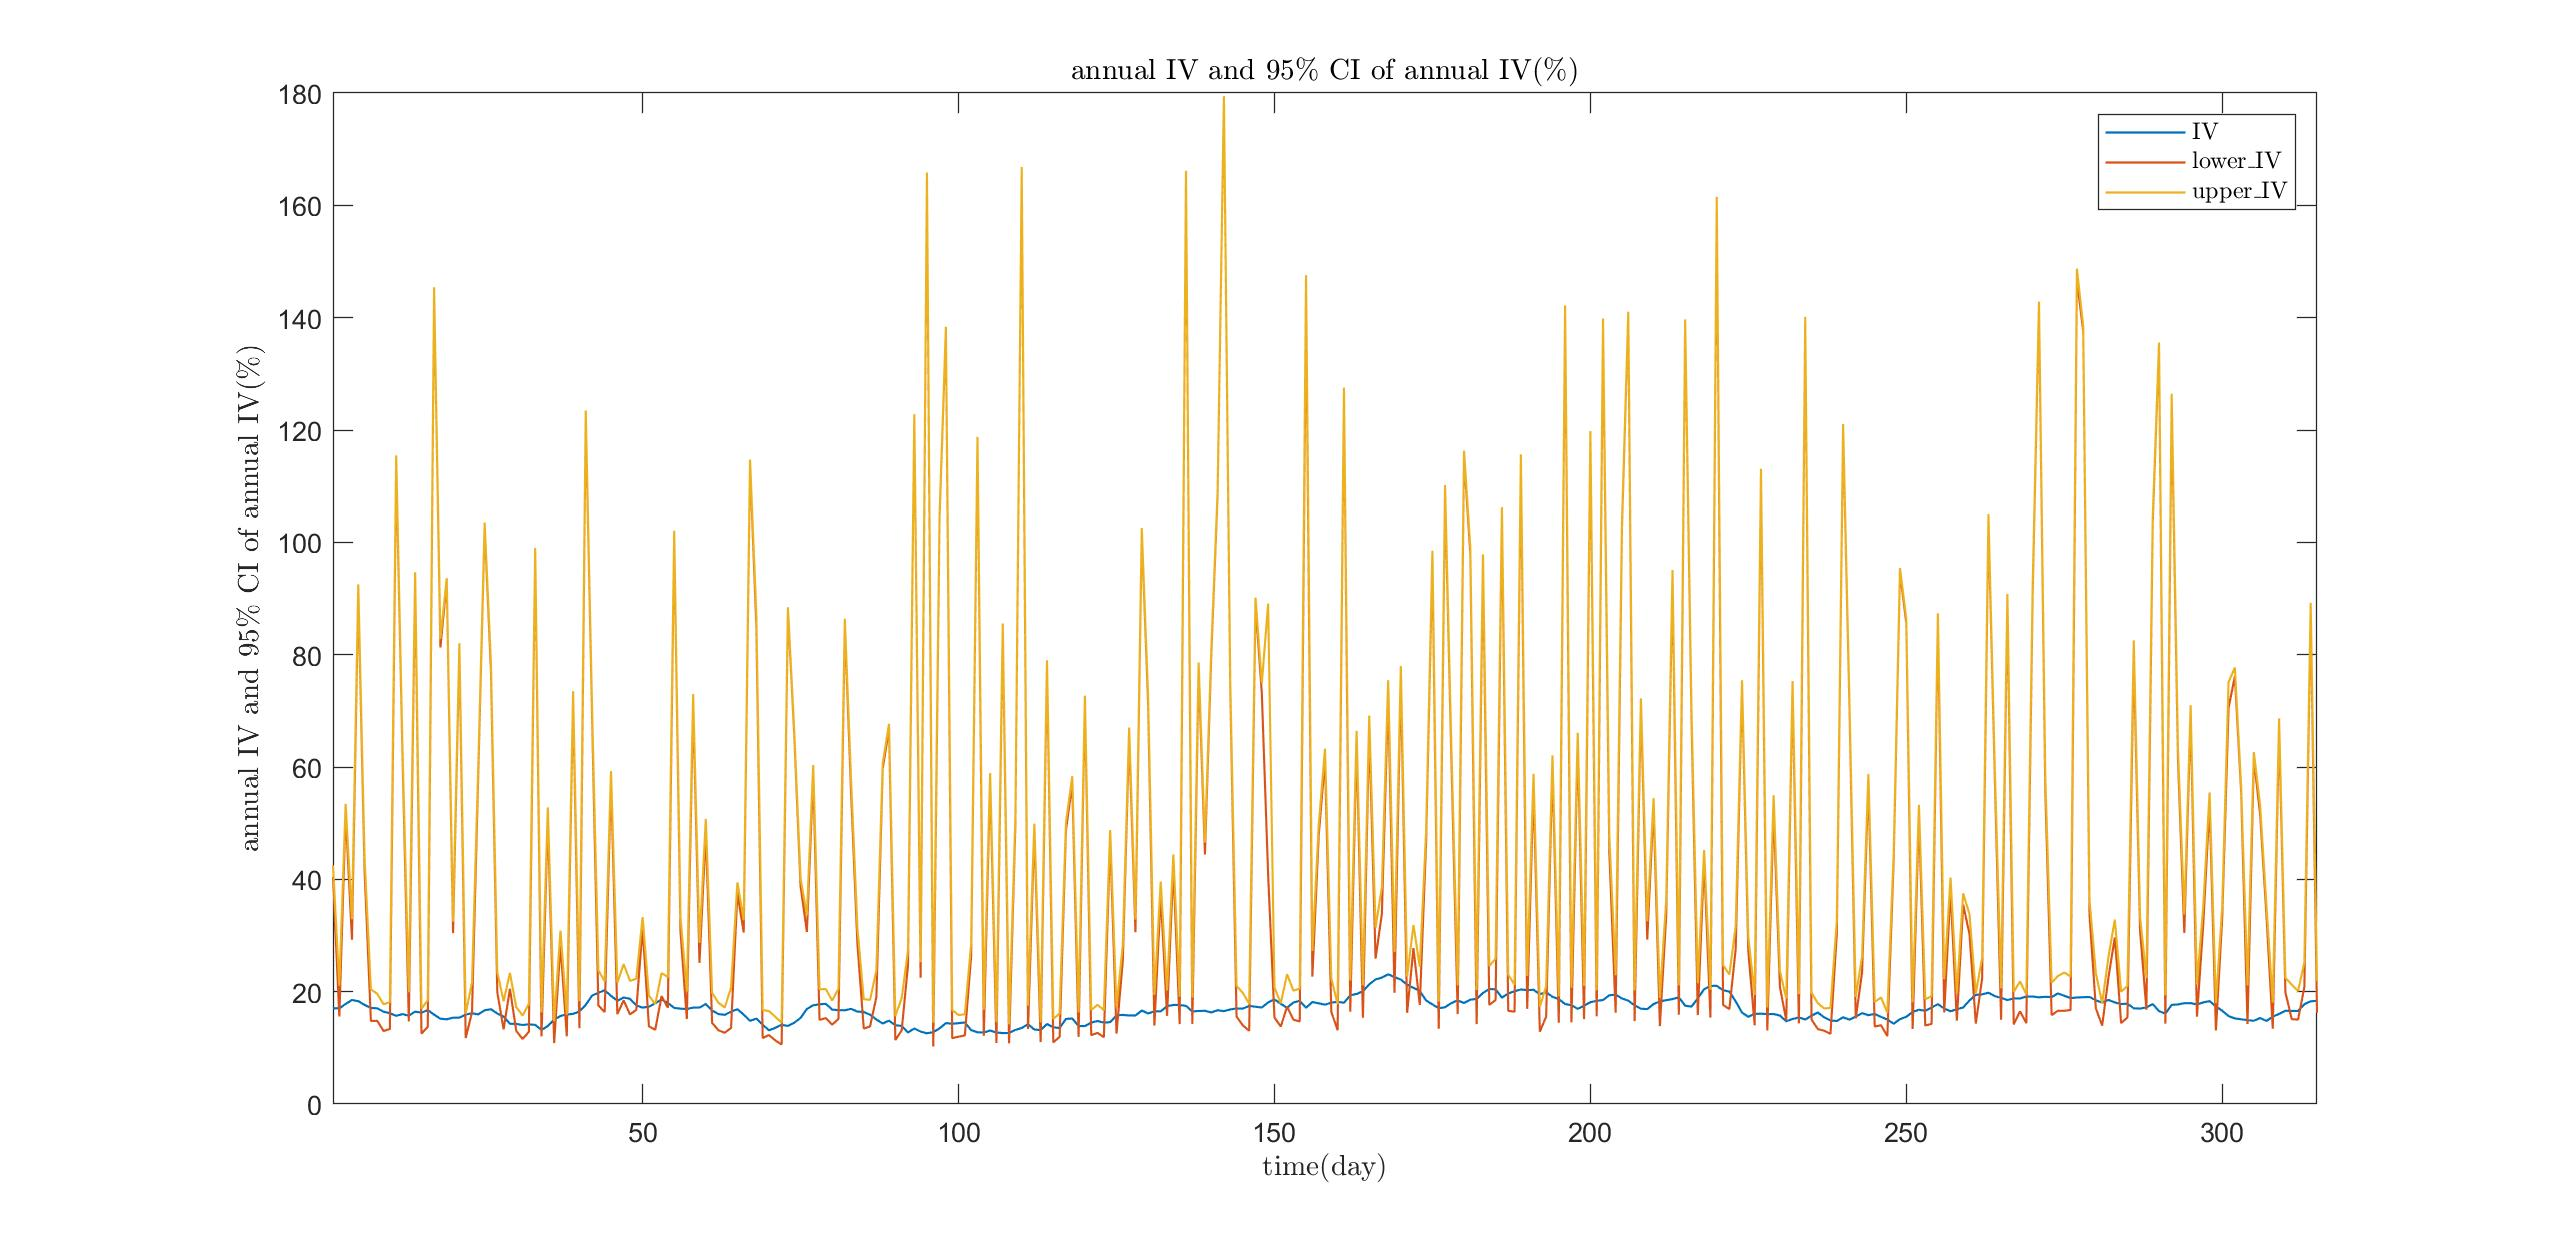
\includegraphics[width=10cm]{figures/p3_ex3_i.jpg}
            \caption{Estimated confidence interval of annual IV(\%)}
            
        \end{figure}
\begin{enumerate}[label=(\roman*)]
    \item The coverage rate of the confidence interval is 41.27\%;
    \item The cover rate when price with jump is smaller than the case when price does not include jumps.
    \item The cover rate is what I expected, since when we set $\lambda=1$ which means that the probability of day's price includes jump will be 1. In that case, the jump return will constructs major part of daily return. If we still use RV to calculate the confidence interval of IV, the confidence interval will bias more than the case in part H where the jumps are less frequency.
    \item When we fail to account the jump returns, we may regard RV as a unbiased estimator of IV. However, RV is no longer a unbiased estimator for IV now. This incorrect assumption will affect the confidence interval we calculated, and the affect will go up as the frequency of jumps goes up(i.e. $\lambda goes up$). The estimated confidence interval will also bias from the ``true'' confidence interval so the probability that IV falls within the estimated confidence interval will decrease as the frequency of jumps goes up.\\
    
\end{enumerate}



The \textbf{MATLAB} code for function to calculate adjusted volatility with different frequency:
   \lstinputlisting{scripts/p3_ex3.m}

  ~~\\


\end{enumerate}
\end{document}
